\documentclass[10pt,]{krantz}
\usepackage{lmodern}
\usepackage{amssymb,amsmath}
\usepackage{ifxetex,ifluatex}
\usepackage{fixltx2e} % provides \textsubscript
\ifnum 0\ifxetex 1\fi\ifluatex 1\fi=0 % if pdftex
  \usepackage[T1]{fontenc}
  \usepackage[utf8]{inputenc}
\else % if luatex or xelatex
  \ifxetex
    \usepackage{mathspec}
  \else
    \usepackage{fontspec}
  \fi
  \defaultfontfeatures{Ligatures=TeX,Scale=MatchLowercase}
    \setmonofont[Mapping=tex-ansi,Scale=0.7]{Source Code Pro}
\fi
% use upquote if available, for straight quotes in verbatim environments
\IfFileExists{upquote.sty}{\usepackage{upquote}}{}
% use microtype if available
\IfFileExists{microtype.sty}{%
\usepackage[]{microtype}
\UseMicrotypeSet[protrusion]{basicmath} % disable protrusion for tt fonts
}{}
\PassOptionsToPackage{hyphens}{url} % url is loaded by hyperref
\usepackage[unicode=true]{hyperref}
\PassOptionsToPackage{usenames,dvipsnames}{color} % color is loaded by hyperref
\hypersetup{
            pdftitle={R Programming - Lecture Notes},
            pdfauthor={Kyun-Seop Bae, Sungpil Han},
            colorlinks=true,
            linkcolor=Maroon,
            citecolor=Blue,
            urlcolor=Blue,
            breaklinks=true}
\urlstyle{same}  % don't use monospace font for urls
\usepackage{natbib}
\bibliographystyle{apalike}
\usepackage{color}
\usepackage{fancyvrb}
\newcommand{\VerbBar}{|}
\newcommand{\VERB}{\Verb[commandchars=\\\{\}]}
\DefineVerbatimEnvironment{Highlighting}{Verbatim}{commandchars=\\\{\}}
% Add ',fontsize=\small' for more characters per line
\usepackage{framed}
\definecolor{shadecolor}{RGB}{248,248,248}
\newenvironment{Shaded}{\begin{snugshade}}{\end{snugshade}}
\newcommand{\KeywordTok}[1]{\textcolor[rgb]{0.13,0.29,0.53}{\textbf{#1}}}
\newcommand{\DataTypeTok}[1]{\textcolor[rgb]{0.13,0.29,0.53}{#1}}
\newcommand{\DecValTok}[1]{\textcolor[rgb]{0.00,0.00,0.81}{#1}}
\newcommand{\BaseNTok}[1]{\textcolor[rgb]{0.00,0.00,0.81}{#1}}
\newcommand{\FloatTok}[1]{\textcolor[rgb]{0.00,0.00,0.81}{#1}}
\newcommand{\ConstantTok}[1]{\textcolor[rgb]{0.00,0.00,0.00}{#1}}
\newcommand{\CharTok}[1]{\textcolor[rgb]{0.31,0.60,0.02}{#1}}
\newcommand{\SpecialCharTok}[1]{\textcolor[rgb]{0.00,0.00,0.00}{#1}}
\newcommand{\StringTok}[1]{\textcolor[rgb]{0.31,0.60,0.02}{#1}}
\newcommand{\VerbatimStringTok}[1]{\textcolor[rgb]{0.31,0.60,0.02}{#1}}
\newcommand{\SpecialStringTok}[1]{\textcolor[rgb]{0.31,0.60,0.02}{#1}}
\newcommand{\ImportTok}[1]{#1}
\newcommand{\CommentTok}[1]{\textcolor[rgb]{0.56,0.35,0.01}{\textit{#1}}}
\newcommand{\DocumentationTok}[1]{\textcolor[rgb]{0.56,0.35,0.01}{\textbf{\textit{#1}}}}
\newcommand{\AnnotationTok}[1]{\textcolor[rgb]{0.56,0.35,0.01}{\textbf{\textit{#1}}}}
\newcommand{\CommentVarTok}[1]{\textcolor[rgb]{0.56,0.35,0.01}{\textbf{\textit{#1}}}}
\newcommand{\OtherTok}[1]{\textcolor[rgb]{0.56,0.35,0.01}{#1}}
\newcommand{\FunctionTok}[1]{\textcolor[rgb]{0.00,0.00,0.00}{#1}}
\newcommand{\VariableTok}[1]{\textcolor[rgb]{0.00,0.00,0.00}{#1}}
\newcommand{\ControlFlowTok}[1]{\textcolor[rgb]{0.13,0.29,0.53}{\textbf{#1}}}
\newcommand{\OperatorTok}[1]{\textcolor[rgb]{0.81,0.36,0.00}{\textbf{#1}}}
\newcommand{\BuiltInTok}[1]{#1}
\newcommand{\ExtensionTok}[1]{#1}
\newcommand{\PreprocessorTok}[1]{\textcolor[rgb]{0.56,0.35,0.01}{\textit{#1}}}
\newcommand{\AttributeTok}[1]{\textcolor[rgb]{0.77,0.63,0.00}{#1}}
\newcommand{\RegionMarkerTok}[1]{#1}
\newcommand{\InformationTok}[1]{\textcolor[rgb]{0.56,0.35,0.01}{\textbf{\textit{#1}}}}
\newcommand{\WarningTok}[1]{\textcolor[rgb]{0.56,0.35,0.01}{\textbf{\textit{#1}}}}
\newcommand{\AlertTok}[1]{\textcolor[rgb]{0.94,0.16,0.16}{#1}}
\newcommand{\ErrorTok}[1]{\textcolor[rgb]{0.64,0.00,0.00}{\textbf{#1}}}
\newcommand{\NormalTok}[1]{#1}
\usepackage{longtable,booktabs}
% Fix footnotes in tables (requires footnote package)
\IfFileExists{footnote.sty}{\usepackage{footnote}\makesavenoteenv{long table}}{}
\usepackage{graphicx,grffile}
\makeatletter
\def\maxwidth{\ifdim\Gin@nat@width>\linewidth\linewidth\else\Gin@nat@width\fi}
\def\maxheight{\ifdim\Gin@nat@height>\textheight\textheight\else\Gin@nat@height\fi}
\makeatother
% Scale images if necessary, so that they will not overflow the page
% margins by default, and it is still possible to overwrite the defaults
% using explicit options in \includegraphics[width, height, ...]{}
\setkeys{Gin}{width=\maxwidth,height=\maxheight,keepaspectratio}
\IfFileExists{parskip.sty}{%
\usepackage{parskip}
}{% else
\setlength{\parindent}{0pt}
\setlength{\parskip}{6pt plus 2pt minus 1pt}
}
\setlength{\emergencystretch}{3em}  % prevent overfull lines
\providecommand{\tightlist}{%
  \setlength{\itemsep}{0pt}\setlength{\parskip}{0pt}}
\setcounter{secnumdepth}{5}
% Redefines (sub)paragraphs to behave more like sections
\ifx\paragraph\undefined\else
\let\oldparagraph\paragraph
\renewcommand{\paragraph}[1]{\oldparagraph{#1}\mbox{}}
\fi
\ifx\subparagraph\undefined\else
\let\oldsubparagraph\subparagraph
\renewcommand{\subparagraph}[1]{\oldsubparagraph{#1}\mbox{}}
\fi

% set default figure placement to htbp
\makeatletter
\def\fps@figure{htbp}
\makeatother

\usepackage{booktabs}
\usepackage{longtable}
\usepackage[bf,singlelinecheck=off]{caption}

\usepackage{kotex}

\setmainfont[UprightFeatures={SmallCapsFont=AlegreyaSC-Regular}]{Alegreya}

\usepackage{framed,color}
\definecolor{shadecolor}{RGB}{248,248,248}

\renewcommand{\textfraction}{0.05}
\renewcommand{\topfraction}{0.8}
\renewcommand{\bottomfraction}{0.8}
\renewcommand{\floatpagefraction}{0.75}

\renewenvironment{quote}{\begin{VF}}{\end{VF}}
\let\oldhref\href
\renewcommand{\href}[2]{#2\footnote{\url{#1}}}

\ifxetex
  \usepackage{letltxmacro}
  \setlength{\XeTeXLinkMargin}{1pt}
  \LetLtxMacro\SavedIncludeGraphics\includegraphics
  \def\includegraphics#1#{% #1 catches optional stuff (star/opt. arg.)
    \IncludeGraphicsAux{#1}%
  }%
  \newcommand*{\IncludeGraphicsAux}[2]{%
    \XeTeXLinkBox{%
      \SavedIncludeGraphics#1{#2}%
    }%
  }%
\fi

\makeatletter
\newenvironment{kframe}{%
\medskip{}
\setlength{\fboxsep}{.8em}
 \def\at@end@of@kframe{}%
 \ifinner\ifhmode%
  \def\at@end@of@kframe{\end{minipage}}%
  \begin{minipage}{\columnwidth}%
 \fi\fi%
 \def\FrameCommand##1{\hskip\@totalleftmargin \hskip-\fboxsep
 \colorbox{shadecolor}{##1}\hskip-\fboxsep
     % There is no \\@totalrightmargin, so:
     \hskip-\linewidth \hskip-\@totalleftmargin \hskip\columnwidth}%
 \MakeFramed {\advance\hsize-\width
   \@totalleftmargin\z@ \linewidth\hsize
   \@setminipage}}%
 {\par\unskip\endMakeFramed%
 \at@end@of@kframe}
\makeatother

\renewenvironment{Shaded}{\begin{kframe}}{\end{kframe}}

\newenvironment{rmdblock}[1]
  {
  \begin{itemize}
  \renewcommand{\labelitemi}{
    \raisebox{-.7\height}[0pt][0pt]{
      {\setkeys{Gin}{width=3em,keepaspectratio}\includegraphics{images/#1}}
    }
  }
  \setlength{\fboxsep}{1em}
  \begin{kframe}
  \item
  }
  {
  \end{kframe}
  \end{itemize}
  }
\newenvironment{rmdnote}
  {\begin{rmdblock}{note}}
  {\end{rmdblock}}
\newenvironment{rmdcaution}
  {\begin{rmdblock}{caution}}
  {\end{rmdblock}}
\newenvironment{rmdimportant}
  {\begin{rmdblock}{important}}
  {\end{rmdblock}}
\newenvironment{rmdtip}
  {\begin{rmdblock}{tip}}
  {\end{rmdblock}}
\newenvironment{rmdwarning}
  {\begin{rmdblock}{warning}}
  {\end{rmdblock}}

\usepackage{makeidx}
\makeindex

\urlstyle{tt}

\usepackage{amsthm}
\makeatletter
\def\thm@space@setup{%
  \thm@preskip=8pt plus 2pt minus 4pt
  \thm@postskip=\thm@preskip
}
\makeatother

\frontmatter

\title{R Programming - Lecture Notes}
\author{Kyun-Seop Bae, Sungpil Han}
\date{2017-04-10}

\usepackage{amsthm}
\newtheorem{theorem}{Theorem}[chapter]
\newtheorem{lemma}{Lemma}[chapter]
\theoremstyle{definition}
\newtheorem{definition}{Definition}[chapter]
\newtheorem{corollary}{Corollary}[chapter]
\newtheorem{proposition}{Proposition}[chapter]
\theoremstyle{definition}
\newtheorem{example}{Example}[chapter]
\theoremstyle{remark}
\newtheorem*{remark}{Remark}
\begin{document}
\maketitle

%\cleardoublepage\newpage\thispagestyle{empty}\null
%\cleardoublepage\newpage\thispagestyle{empty}\null
%\cleardoublepage\newpage
\thispagestyle{empty}
\begin{center}
\includegraphics{images/cover.pdf}
\end{center}

\setlength{\abovedisplayskip}{-1pt}
\setlength{\abovedisplayshortskip}{-1pt}

{
\hypersetup{linkcolor=black}
\setcounter{tocdepth}{2}
\tableofcontents
}
\listoftables
\listoffigures
\chapter*{Preface}\label{preface}


안녕하십니까?

2017년 1학기 울산대학교 의학과 대학원 수업 \texttt{R\ Programming} 과목
담당교수 배균섭입니다.

R은 \url{http://cran.r-project.org} 에서 다운로드받아 설치할 수
있습니다. 역시 같은 사이트에서 Manual이 나와 있으니 참고하시기 바랍니다.
구글에서 `R Programming pdf'와 같은 키워드로 검색하시면 많은 자료를 보실
수 있습니다.

첨부한
\href{https://groups.google.com/a/acr.kr/group/r/attach/409db97bf453a/R.stx?part=0.1\&authuser=0}{R.stx}
파일은 AcroEdit이라는 editor에서 사용할 syntax highlighting용 구문
파일입니다. \url{http://www.acrosoft.pe.kr} 에서 다운로드 받아
설치하시기 바랍니다. AcroEdit대신 notepad++를 선호하시는 분은 그대로
사용하셔도 됩니다.

저는 RStudio, tinnR 등을 이용해서 강의하지 않습니다만, 필요하신 분은
쓰셔도 괜찮습니다. 향후 R package 작성을 위해서는 MiKTeX와 Rtools를
설치하십시오.

추가로 말씀드리자면, \url{http://www.coursera.org} 에 많은 R 강좌가
개설되어 있습니다. Specialization course로 들어가면 유로이지만,
(Specialization course는 여러 개의 과목이 합쳐져 있는 것입니다.) 개별
과목을 검색해서 들어가면, 무료로도 볼 수 있습니다. (대신 시험을 칠 수
없거나, certificate를 받을 수 없습니다.)

좋은 강좌가 많으니 많이 활용하시기 바립니다.

강의 장소에 불편함이 많은 것으로 생각되어, 다음과 같이 Skype 모임을
개설하였습니다. 사정상 원거리에서 오시기 불편한 분들은 활용하시기
바랍니다. 출석은 화면을 캡쳐하거나 휴대폰으로 찍은 뒤
\href{mailto:sec@acp.kr}{\nolinkurl{sec@acp.kr}},
\href{mailto:shan@acp.kr로}{\nolinkurl{shan@acp.kr로}} 보내주시면
출석으로 인정해 드립니다.

Skype 모임 참가 \url{https://meet.lync.com/uucp-acp/ksbae/SKGJ3BNQ}

2017년 3월, 배균섭 배상

The online version of this book is licensed under the
\href{http://creativecommons.org/licenses/by-nc-sa/4.0/}{Creative
Commons Attribution-NonCommercial-ShareAlike 4.0 International License}.

\begin{figure}
\centering
\includegraphics{images/by-nc-sa.png}
\caption{Creative Commons License}
\end{figure}

\section*{Teaching Assistant}\label{teaching-assistant}


안녕하십니까? 서울아산병원 임상약리학과 전공의 한성필입니다. 수업과
관련된 여러 제반 업무를 담당하고 있습니다. 언제든 의문사항 있으면
\href{mailto:r@acr.kr}{\nolinkurl{r@acr.kr}} 로 전체 메일 보내시거나
교수님 \href{mailto:k@acr.kr}{\nolinkurl{k@acr.kr}} 혹은 제 개인 메일
\href{mailto:shan@acp.kr로}{\nolinkurl{shan@acp.kr로}} 연락해 주십시오.

교수님께서 세우신 방침에 따라 수업시간에 출석을 부르지 않을 예정입니다.
수강하시는 화면(Skype)을 휴대폰으로 사진 찍으시거나 강의실의 스크린을
사진으로 촬영하셔서 \href{mailto:sec@acp.kr}{\nolinkurl{sec@acp.kr}} /
\href{mailto:shan@acp.kr}{\nolinkurl{shan@acp.kr}} 로 동시에 보내주시면
됩니다. 가급적 ``2017-03-31 한성필 출석'' 과 같은 식의 제목을 유지해
주시면 처리하는데 큰 도움이 될 것 같습니다.

\textbf{출석 체크를 위해 전체메일을 사용하지 말아주십시오!}

아울러 수업 중에 사용한 코드/스크립트를 사용하여 R의 패키지인
\texttt{bookdown}을 사용해 웹북을 제작 중에 있습니다. \citep{R-bookdown}
\index{bookdown} 여러분이 읽고 있는 이 책 자체가 R 코드의 일종인
\texttt{Rmarkdown}의 결과물이라고 보시면 됩니다.
\href{https://github.com/asancpt/Rprogramming}{Github 저장소}가 있으니
소스 코드를 보실 수 있습니다. 누구나 소스를 편집하여
\texttt{Pull\ Request}를 요청할 수 있으므로 혹시 Github를 사용하셔서
웹북의 질을 높이고자 하시는 수강생 선생님들께서는 도움을 주십시오.
\index{Github}

감사합니다.

2017년 3월, 한성필 올림

\section*{FAQ}\label{faq}


\subsection*{접속 관련}\label{-}


\begin{quote}
Q. 스카이프를 한번도 안써봐서 이참에 사용법을 배우고있는데, 수업시작시에
상대방을 어떻게 검색해서 들어가면 될지 알려주시면 감사하겠습니다.
\end{quote}

\begin{quote}
Q. 온라인 수강시 접속하는 스카이프 주소는 무엇인지요?
\end{quote}

\url{https://meet.lync.com/uucp-acp/ksbae/SKGJ3BNQ}

Chrome 등 웹브라우저에서 위 주소를 입력하면 직접 대화방으로 연결됩니다.
(검색할 필요 없습니다.) 처음 설치시에는 Add-on이 설치될 수 있습니다.
MacOS Sierra, Win7, Win10에서 Chrome, Internet Explorer 등을 사용하여
테스트해 보았고 모두 잘 동작하였습니다. 대부분의 경우 Skype For Business
계정이 없을 것으로 생각되는데 따로 로그인할 필요 없습니다.

수업 시작 30분 전부터 대화방을 개설해 놓도록 하겠습니다.

\url{https://groups.google.com/a/acr.kr/d/msg/r/nUkrE37W2kQ/waG-FkM_BgAJ}
교수님께서 처음 보낸 메일을 참고해 주십시오.

\begin{quote}
Q. 앞으로 수업은 지난 첫수업처럼 계속 온라인 수강이 가능한 것인가요?
\end{quote}

네, 계속 온라인으로 가능합니다.

\begin{quote}
Q. 저도 웹캠을 설치하여야 하여야 하나요?
\end{quote}

설치할 필요 없습니다. 오히려 수강자의 웹캠의 전원을 꺼두시길
권고드립니다.

\begin{quote}
Q. 수강전 온라인 강의 테스트 해볼 수 있나요?
\end{quote}

수업 시작 30분 전부터 대화방을 개설하여 놓도록 하겠습니다.

\subsection*{출석관련}


\begin{quote}
Q. 미국학회 참석으로 수업시간이 귀국행 비행기 기내에 있을거같아 출석이
안될것 같습니다. 방법이 있을지요?
\end{quote}

결석 사유서를 제출해 주시면 출석 처리 하겠습니다.
\href{http://www.medulsan.ac.kr/graduate/?mid=72\&curpage=files}{대학원
홈페이지 참고 바랍니다.} 이 링크로 들어가시면 가장 위에 있습니다.
(\texttt{결석사유서.hwp}) 참고로 수업 영상은 녹화하여 Youtube에 비공개
링크를 만들 예정이라서 추후에 관련 영상을 시청할 수 있을 것 같습니다.
결석사유서를 제출한다고 100\% 출석이 인정되는 것은 아닙니다. 이것이
기본적으로는 offline강의이기 때문에 강의시간에 강의실에 있든지, 또는
온라인으로 접속해 있어야 합니다. 출석사유서를 제출하거나, 추후 동영상
시청을 해서 그 증거(사진)을 제출하는 경우에 감점을 줄여드릴 수 있습니다.
예를 들어, 결석시에는 2점 감점인데, 결석사유서를 제출하면 1점만
감점한다는지, 동영상을 보면 0.5점만 감점한다는지 하는 것입니다. 결석
사유서 제출 시 출석 처리 원칙에 대한 설명을 드리오니, 참고하시길
바랍니다.

\subsection*{과제 관련}\label{-}


\begin{quote}
Q. 과제물이 있다고 들었는데 언제 assign하게 되는지요?
\end{quote}

과제물은 빨라야 5주차 이후에 나갑니다.

\subsection*{Coursera 관련}\label{coursera-}


\begin{quote}
Q. 첫 수업 때, certification 관련 말씀을 하셨는데, 정확히 coursera
사이트에서 어떤 것을 듣고, 제출을 해야하는지 궁금합니다. (비슷한 내용이
많아, 어떤것을 들어야하는지 헷갈립니다.) \index{Coursera}
\end{quote}

Coursera는 꼭 어느 것을 들어야 하는 것은 아니고, R programming과 관련된
것이라면 자유로이 골라서 들으면 됩니다. 대표적인 두 가지만 들자면 다음과
같습니다.

\begin{itemize}
\tightlist
\item
  \url{https://www.coursera.org/learn/r-programming}
\item
  \url{https://www.coursera.org/learn/r-programming-environment}
\end{itemize}

\begin{quote}
Q. Coursera 강의를 듣고 증명서를 내면 출석을 얼마나 커버할 수
있을런지요?
\end{quote}

Coursera는 출석 커버보다는 grade를 올려 주기 위한 것입니다. 출석은
Skype로 커버해야 합니다. 출석의 성적 반영비율은 25\%이지만, 규정상 4회
이상 결석이면 성적이 나갈 수 없습니다.

\section*{Syllabus}\label{syllabus}


2017년 4월 10일 개정된 수업계획서입니다.

\begin{figure}
\centering
\includegraphics{inst/syllabus/syllabus_rev-0.png}
\caption{Syllabus page 1}
\end{figure}

\begin{figure}
\centering
\includegraphics{inst/syllabus/syllabus_rev-1.png}
\caption{Syllabus page 1}
\end{figure}

\mainmatter

\chapter{R language}\label{r-language}

\begin{quote}
2017-03-15 배균섭 교수님 강의
\end{quote}

\href{https://cran.r-project.org/doc/manuals/r-release/R-lang.pdf}{R
Language Definition}의 초반 내용에 대해 설명하였습니다.

\chapter{Graphics}\label{graphics}

\begin{quote}
2017-03-22 임형석 교수님 강의
\end{quote}

R을 사용해 그림 그리는 방법에 대해 알아보겠습니다.

\section{Introduction}\label{introduction}

\begin{itemize}
\tightlist
\item
  상위수준 그림 함수는 그림을 생성한다.
\item
  하위수준 그림 함수는 기존의 그림에 그림을 추가한다.
\end{itemize}

\section{상위수준 그림 함수}\label{upper}

\subsection{상위수준 그림 함수의 주요 인자
(arguments)}\label{-----arguments}

\begin{itemize}
\tightlist
\item
  main : 제목
\item
  xlab/ylab : x축 및 y축 레이블
\item
  xlim/ylim : x축 및 y축 범위
\item
  col : 색깔
\item
  lty : 선 모양
\item
  pch : 점 모양
\item
  cex : 그림 성분의 크기
\item
  lwd : 선 굵기
\item
  type : 그림 타입
\end{itemize}

\begin{Shaded}
\begin{Highlighting}[]
\NormalTok{dta <-}\StringTok{ }\KeywordTok{read.csv}\NormalTok{(}\StringTok{"PK.csv"}\NormalTok{)}
\KeywordTok{head}\NormalTok{(dta)}
\NormalTok{##   ID TIME AMT    DV MDV}
\NormalTok{## 1  1 0.00   0  0.00   0}
\NormalTok{## 2  1 0.00   4  0.00   1}
\NormalTok{## 3  1 0.33   0  9.40   0}
\NormalTok{## 4  1 0.66   0 13.71   0}
\NormalTok{## 5  1 1.00   0 16.52   0}
\NormalTok{## 6  1 1.50   0 29.36   0}
\KeywordTok{str}\NormalTok{(dta)}
\NormalTok{## 'data.frame':    456 obs. of  5 variables:}
\NormalTok{##  $ ID  : num  1 1 1 1 1 1 1 1 1 1 ...}
\NormalTok{##  $ TIME: num  0 0 0.33 0.66 1 1.5 2 3 4 6 ...}
\NormalTok{##  $ AMT : num  0 4 0 0 0 0 0 0 0 0 ...}
\NormalTok{##  $ DV  : num  0 0 9.4 13.7 16.5 ...}
\NormalTok{##  $ MDV : num  0 1 0 0 0 0 0 0 0 0 ...}
\end{Highlighting}
\end{Shaded}

\subsection{scatter plot}\label{scatter-plot}

\begin{Shaded}
\begin{Highlighting}[]

\KeywordTok{plot}\NormalTok{(dta}\OperatorTok{$}\NormalTok{TIME[dta}\OperatorTok{$}\NormalTok{MDV}\OperatorTok{==}\DecValTok{0}\NormalTok{], dta}\OperatorTok{$}\NormalTok{DV[dta}\OperatorTok{$}\NormalTok{MDV}\OperatorTok{==}\DecValTok{0}\NormalTok{])}
\end{Highlighting}
\end{Shaded}

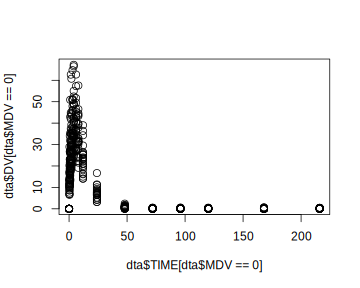
\includegraphics{Rprogramming_files/figure-latex/unnamed-chunk-3-1.png}

\begin{Shaded}
\begin{Highlighting}[]

\KeywordTok{plot}\NormalTok{(dta}\OperatorTok{$}\NormalTok{TIME[dta}\OperatorTok{$}\NormalTok{MDV}\OperatorTok{==}\DecValTok{0}\NormalTok{], dta}\OperatorTok{$}\NormalTok{DV[dta}\OperatorTok{$}\NormalTok{MDV}\OperatorTok{==}\DecValTok{0}\NormalTok{], }\DataTypeTok{log=}\StringTok{"y"}\NormalTok{)}
\NormalTok{## Warning in xy.coords(x, y, xlabel, ylabel, log): 86 y}
\NormalTok{## values <= 0 omitted from logarithmic plot}
\end{Highlighting}
\end{Shaded}

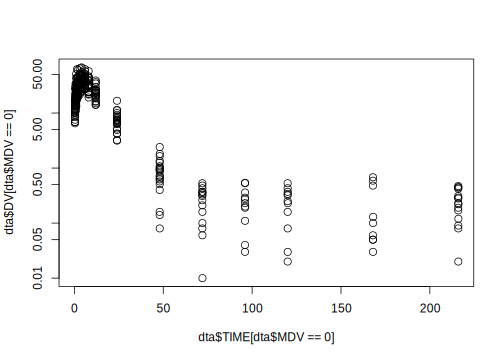
\includegraphics{Rprogramming_files/figure-latex/unnamed-chunk-3-2.png}

\begin{Shaded}
\begin{Highlighting}[]

\KeywordTok{plot}\NormalTok{(dta}\OperatorTok{$}\NormalTok{TIME[dta}\OperatorTok{$}\NormalTok{MDV}\OperatorTok{==}\DecValTok{0}\NormalTok{], }\KeywordTok{log}\NormalTok{(dta}\OperatorTok{$}\NormalTok{DV[dta}\OperatorTok{$}\NormalTok{MDV}\OperatorTok{==}\DecValTok{0}\NormalTok{]))}
\end{Highlighting}
\end{Shaded}

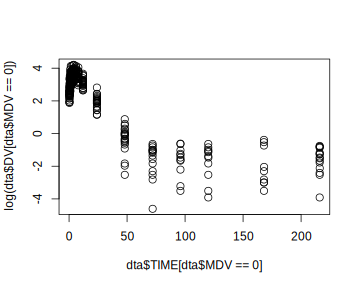
\includegraphics{Rprogramming_files/figure-latex/unnamed-chunk-3-3.png}

\begin{Shaded}
\begin{Highlighting}[]

\KeywordTok{plot}\NormalTok{(dta}\OperatorTok{$}\NormalTok{TIME[dta}\OperatorTok{$}\NormalTok{MDV}\OperatorTok{==}\DecValTok{0}\NormalTok{], dta}\OperatorTok{$}\NormalTok{DV[dta}\OperatorTok{$}\NormalTok{MDV}\OperatorTok{==}\DecValTok{0}\NormalTok{]}
\NormalTok{     , }\DataTypeTok{xlab=}\StringTok{"Time (hr)"}\NormalTok{, }\DataTypeTok{ylab=}\StringTok{"Concentration (ng/mL)"} 
\NormalTok{     , }\DataTypeTok{type=}\StringTok{"o"}\NormalTok{, }\DataTypeTok{pch=}\DecValTok{2}\NormalTok{, }\DataTypeTok{col=}\DecValTok{1}\NormalTok{, }\DataTypeTok{main=}\StringTok{"PK time-course of Drug X"}
\NormalTok{     , }\DataTypeTok{xlim =}\KeywordTok{c}\NormalTok{(}\OperatorTok{-}\DecValTok{2}\NormalTok{,}\DecValTok{218}\NormalTok{), }\DataTypeTok{ylim=}\KeywordTok{c}\NormalTok{(}\DecValTok{0}\NormalTok{,}\DecValTok{80}\NormalTok{))}
\end{Highlighting}
\end{Shaded}

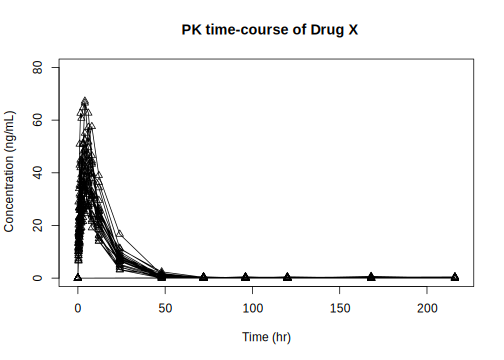
\includegraphics{Rprogramming_files/figure-latex/unnamed-chunk-3-4.png}

\begin{Shaded}
\begin{Highlighting}[]

\KeywordTok{plot}\NormalTok{(dta}\OperatorTok{$}\NormalTok{TIME[dta}\OperatorTok{$}\NormalTok{MDV}\OperatorTok{==}\DecValTok{0}\NormalTok{], dta}\OperatorTok{$}\NormalTok{DV[dta}\OperatorTok{$}\NormalTok{MDV}\OperatorTok{==}\DecValTok{0}\NormalTok{], }\DataTypeTok{axes=}\NormalTok{F,}
\NormalTok{     , }\DataTypeTok{xlab=}\StringTok{"Time (hr)"}\NormalTok{, }\DataTypeTok{ylab=}\StringTok{"Concentration (ng/mL)"} 
\NormalTok{     , }\DataTypeTok{type=}\StringTok{"o"}\NormalTok{, }\DataTypeTok{pch=}\DecValTok{2}\NormalTok{, }\DataTypeTok{col=}\DecValTok{1}\NormalTok{, }\DataTypeTok{main=}\StringTok{"PK time-course of Drug X"}
\NormalTok{     , }\DataTypeTok{xlim =}\KeywordTok{c}\NormalTok{(}\OperatorTok{-}\DecValTok{2}\NormalTok{,}\DecValTok{218}\NormalTok{), }\DataTypeTok{ylim=}\KeywordTok{c}\NormalTok{(}\DecValTok{0}\NormalTok{,}\DecValTok{80}\NormalTok{))}
\KeywordTok{axis}\NormalTok{(}\DecValTok{1}\NormalTok{, }\DataTypeTok{at=}\KeywordTok{seq}\NormalTok{(}\DecValTok{0}\NormalTok{, }\DecValTok{218}\NormalTok{, }\DecValTok{24}\NormalTok{))}
\KeywordTok{axis}\NormalTok{(}\DecValTok{2}\NormalTok{)}
\KeywordTok{box}\NormalTok{()}
\end{Highlighting}
\end{Shaded}

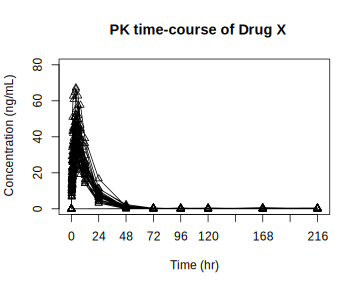
\includegraphics{Rprogramming_files/figure-latex/unnamed-chunk-3-5.png}

\subsection{Histogram}\label{histogram}

\begin{Shaded}
\begin{Highlighting}[]

\NormalTok{d.demog <-}\StringTok{ }\KeywordTok{read.csv}\NormalTok{(}\StringTok{"DEMOG.csv"}\NormalTok{)}

\KeywordTok{hist}\NormalTok{(d.demog}\OperatorTok{$}\NormalTok{HT)}
\end{Highlighting}
\end{Shaded}

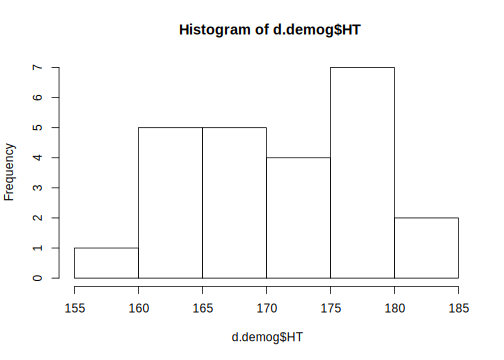
\includegraphics{Rprogramming_files/figure-latex/unnamed-chunk-4-1.png}

\begin{Shaded}
\begin{Highlighting}[]

\KeywordTok{hist}\NormalTok{(d.demog}\OperatorTok{$}\NormalTok{HT, }\DataTypeTok{breaks=}\DecValTok{10}\NormalTok{)}
\KeywordTok{hist}\NormalTok{(d.demog}\OperatorTok{$}\NormalTok{HT, }\DataTypeTok{nclass=}\DecValTok{10}\NormalTok{)}
\end{Highlighting}
\end{Shaded}

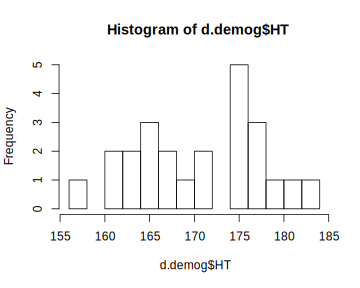
\includegraphics{Rprogramming_files/figure-latex/unnamed-chunk-4-2.png}

\subsubsection{with density line}\label{with-density-line}

\begin{Shaded}
\begin{Highlighting}[]
\KeywordTok{hist}\NormalTok{ (d.demog}\OperatorTok{$}\NormalTok{HT, }\DataTypeTok{probability=}\OtherTok{TRUE}\NormalTok{, }\DataTypeTok{breaks=}\DecValTok{10}\NormalTok{)}
\KeywordTok{lines}\NormalTok{(}\KeywordTok{density}\NormalTok{(d.demog}\OperatorTok{$}\NormalTok{HT))}
\end{Highlighting}
\end{Shaded}

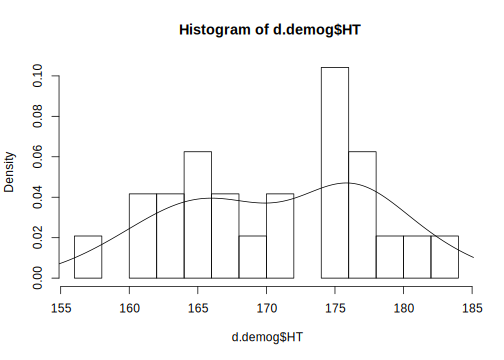
\includegraphics{Rprogramming_files/figure-latex/unnamed-chunk-5-1.png}

\begin{Shaded}
\begin{Highlighting}[]


\KeywordTok{hist}\NormalTok{ (d.demog}\OperatorTok{$}\NormalTok{HT, }\DataTypeTok{probability=}\OtherTok{TRUE}\NormalTok{, }\DataTypeTok{breaks=}\DecValTok{9}\NormalTok{, }\DataTypeTok{xaxt=}\StringTok{"n"}
\NormalTok{      , }\DataTypeTok{main=}\StringTok{"Histogram for Height"}\NormalTok{, }\DataTypeTok{xlab=}\StringTok{"Height (cm)"}\NormalTok{, }\DataTypeTok{ylab=}\StringTok{"Probability (%)"}\NormalTok{)}
\KeywordTok{axis}\NormalTok{(}\DecValTok{1}\NormalTok{, }\DataTypeTok{at=}\KeywordTok{seq}\NormalTok{(}\KeywordTok{min}\NormalTok{(d.demog}\OperatorTok{$}\NormalTok{HT), }\KeywordTok{max}\NormalTok{(d.demog}\OperatorTok{$}\NormalTok{HT), }\DecValTok{3}\NormalTok{))}
\KeywordTok{lines}\NormalTok{(}\KeywordTok{density}\NormalTok{(d.demog}\OperatorTok{$}\NormalTok{HT))}
\end{Highlighting}
\end{Shaded}

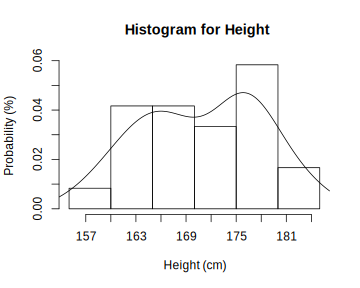
\includegraphics{Rprogramming_files/figure-latex/unnamed-chunk-5-2.png}

\begin{Shaded}
\begin{Highlighting}[]


\KeywordTok{hist}\NormalTok{ (d.demog}\OperatorTok{$}\NormalTok{HT, }\DataTypeTok{probability=}\OtherTok{TRUE}\NormalTok{, }\DataTypeTok{breaks=}\DecValTok{9}\NormalTok{, }\DataTypeTok{xaxt=}\StringTok{"n"}
\NormalTok{      , }\DataTypeTok{main=}\StringTok{"Histogram for Height"}\NormalTok{, }\DataTypeTok{xlab=}\StringTok{"Height (cm)"}\NormalTok{, }\DataTypeTok{ylab=}\StringTok{"Probability (%)"}
\NormalTok{      , }\DataTypeTok{col =} \StringTok{"lightblue"}\NormalTok{, }\DataTypeTok{border =} \StringTok{"pink"}\NormalTok{)}
\KeywordTok{axis}\NormalTok{(}\DecValTok{1}\NormalTok{, }\DataTypeTok{at=}\KeywordTok{seq}\NormalTok{(}\KeywordTok{min}\NormalTok{(d.demog}\OperatorTok{$}\NormalTok{HT), }\KeywordTok{max}\NormalTok{(d.demog}\OperatorTok{$}\NormalTok{HT), }\DecValTok{3}\NormalTok{))}
\KeywordTok{lines}\NormalTok{(}\KeywordTok{density}\NormalTok{(d.demog}\OperatorTok{$}\NormalTok{HT))}
\end{Highlighting}
\end{Shaded}

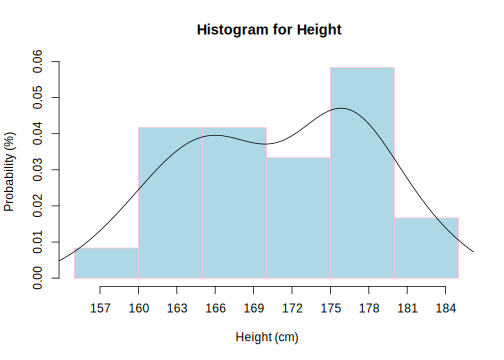
\includegraphics{Rprogramming_files/figure-latex/unnamed-chunk-5-3.png}

\subsection{Box-Whisker Plot}\label{box-whisker-plot}

\begin{Shaded}
\begin{Highlighting}[]
\KeywordTok{boxplot}\NormalTok{(d.demog}\OperatorTok{$}\NormalTok{WT)}
\end{Highlighting}
\end{Shaded}

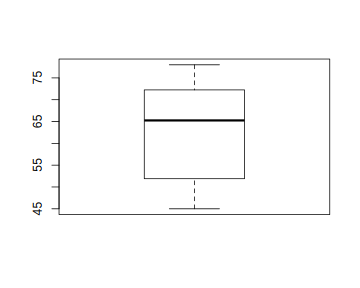
\includegraphics{Rprogramming_files/figure-latex/unnamed-chunk-6-1.png}

\begin{Shaded}
\begin{Highlighting}[]

\KeywordTok{boxplot}\NormalTok{(d.demog}\OperatorTok{$}\NormalTok{WT }\OperatorTok{~}\StringTok{ }\NormalTok{d.demog}\OperatorTok{$}\NormalTok{SEX)}

\KeywordTok{boxplot}\NormalTok{(}\KeywordTok{split}\NormalTok{(d.demog}\OperatorTok{$}\NormalTok{WT, d.demog}\OperatorTok{$}\NormalTok{SEX))}
\end{Highlighting}
\end{Shaded}

\includegraphics{Rprogramming_files/figure-latex/unnamed-chunk-6-2.png}

\begin{Shaded}
\begin{Highlighting}[]

\KeywordTok{boxplot}\NormalTok{(WT }\OperatorTok{~}\StringTok{ }\NormalTok{SEX, }\DataTypeTok{data=}\NormalTok{d.demog)}

\KeywordTok{boxplot}\NormalTok{(d.demog}\OperatorTok{$}\NormalTok{WT }\OperatorTok{~}\StringTok{ }\NormalTok{d.demog}\OperatorTok{$}\NormalTok{SEX}
\NormalTok{        , }\DataTypeTok{names=}\KeywordTok{c}\NormalTok{(}\StringTok{"Male"}\NormalTok{,}\StringTok{"Female"}\NormalTok{), }\DataTypeTok{ylab=}\StringTok{"AGE, year"}\NormalTok{, }\DataTypeTok{ylim=}\KeywordTok{c}\NormalTok{(}\KeywordTok{min}\NormalTok{(d.demog}\OperatorTok{$}\NormalTok{WT)}\OperatorTok{-}\DecValTok{2}\NormalTok{, }\KeywordTok{max}\NormalTok{(d.demog}\OperatorTok{$}\NormalTok{WT)}\OperatorTok{+}\DecValTok{2}\NormalTok{)}
\NormalTok{        , }\DataTypeTok{col=}\StringTok{"pink"}\NormalTok{)}
\end{Highlighting}
\end{Shaded}

\includegraphics{Rprogramming_files/figure-latex/unnamed-chunk-6-3.png}

\begin{Shaded}
\begin{Highlighting}[]

\KeywordTok{boxplot}\NormalTok{(d.demog}\OperatorTok{$}\NormalTok{WT }\OperatorTok{~}\StringTok{ }\NormalTok{d.demog}\OperatorTok{$}\NormalTok{SEX}
\NormalTok{        , }\DataTypeTok{names=}\KeywordTok{c}\NormalTok{(}\StringTok{"Male"}\NormalTok{,}\StringTok{"Female"}\NormalTok{), }\DataTypeTok{ylab=}\StringTok{"AGE, year"}\NormalTok{, }\DataTypeTok{ylim=}\KeywordTok{c}\NormalTok{(}\KeywordTok{min}\NormalTok{(d.demog}\OperatorTok{$}\NormalTok{WT)}\OperatorTok{-}\DecValTok{2}\NormalTok{, }\KeywordTok{max}\NormalTok{(d.demog}\OperatorTok{$}\NormalTok{WT)}\OperatorTok{+}\DecValTok{2}\NormalTok{)}
\NormalTok{        , }\DataTypeTok{col=}\KeywordTok{c}\NormalTok{(}\StringTok{"lightblue"}\NormalTok{, }\StringTok{"salmon"}\NormalTok{), }\DataTypeTok{width=}\KeywordTok{c}\NormalTok{(}\FloatTok{0.6}\NormalTok{, }\DecValTok{1}\NormalTok{))}
\end{Highlighting}
\end{Shaded}

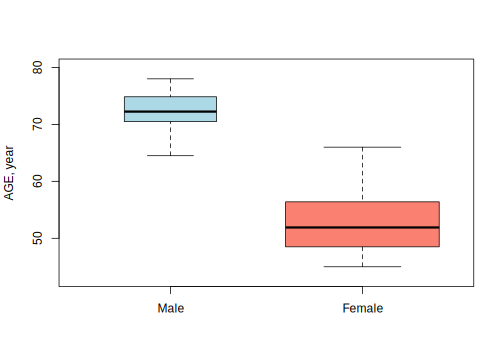
\includegraphics{Rprogramming_files/figure-latex/unnamed-chunk-6-4.png}

-varwidth: if varwidth is TRUE, the boxes are drawn with widths
proportional to the square-roots of the number of observations in the
groups.

\begin{Shaded}
\begin{Highlighting}[]
\KeywordTok{boxplot}\NormalTok{(d.demog}\OperatorTok{$}\NormalTok{WT }\OperatorTok{~}\StringTok{ }\NormalTok{d.demog}\OperatorTok{$}\NormalTok{SEX}
\NormalTok{        , }\DataTypeTok{names=}\KeywordTok{c}\NormalTok{(}\StringTok{"Male"}\NormalTok{,}\StringTok{"Female"}\NormalTok{), }\DataTypeTok{ylab=}\StringTok{"AGE, year"}\NormalTok{, }\DataTypeTok{ylim=}\KeywordTok{c}\NormalTok{(}\KeywordTok{min}\NormalTok{(d.demog}\OperatorTok{$}\NormalTok{WT)}\OperatorTok{-}\DecValTok{2}\NormalTok{, }\KeywordTok{max}\NormalTok{(d.demog}\OperatorTok{$}\NormalTok{WT)}\OperatorTok{+}\DecValTok{2}\NormalTok{)}
\NormalTok{        , }\DataTypeTok{col=}\KeywordTok{c}\NormalTok{(}\StringTok{"lightblue"}\NormalTok{, }\StringTok{"salmon"}\NormalTok{)}
\NormalTok{        , }\DataTypeTok{varwidth=}\OtherTok{TRUE}\NormalTok{)}
\end{Highlighting}
\end{Shaded}

\includegraphics{Rprogramming_files/figure-latex/unnamed-chunk-7-1.png}

\subsection{Bar Plot}\label{bar-plot}

\begin{Shaded}
\begin{Highlighting}[]
\KeywordTok{barplot}\NormalTok{(d.demog}\OperatorTok{$}\NormalTok{HT)}
\end{Highlighting}
\end{Shaded}

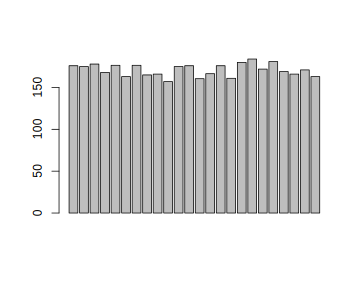
\includegraphics{Rprogramming_files/figure-latex/unnamed-chunk-8-1.png}

\begin{Shaded}
\begin{Highlighting}[]

\NormalTok{VADeaths}
\NormalTok{##       Rural Male Rural Female Urban Male Urban Female}
\NormalTok{## 50-54       11.7          8.7       15.4          8.4}
\NormalTok{## 55-59       18.1         11.7       24.3         13.6}
\NormalTok{## 60-64       26.9         20.3       37.0         19.3}
\NormalTok{## 65-69       41.0         30.9       54.6         35.1}
\NormalTok{## 70-74       66.0         54.3       71.1         50.0}

\KeywordTok{barplot}\NormalTok{(VADeaths, }\DataTypeTok{border =} \StringTok{"dark blue"}\NormalTok{)}
\end{Highlighting}
\end{Shaded}

\includegraphics{Rprogramming_files/figure-latex/unnamed-chunk-8-2.png}

\begin{Shaded}
\begin{Highlighting}[]

\KeywordTok{barplot}\NormalTok{(VADeaths, }\DataTypeTok{col =} \KeywordTok{rainbow}\NormalTok{(}\DecValTok{20}\NormalTok{))}
\end{Highlighting}
\end{Shaded}

\includegraphics{Rprogramming_files/figure-latex/unnamed-chunk-8-3.png}

\begin{Shaded}
\begin{Highlighting}[]

\KeywordTok{barplot}\NormalTok{(VADeaths, }\DataTypeTok{col =} \KeywordTok{heat.colors}\NormalTok{(}\DecValTok{8}\NormalTok{))}
\end{Highlighting}
\end{Shaded}

\includegraphics{Rprogramming_files/figure-latex/unnamed-chunk-8-4.png}

\begin{Shaded}
\begin{Highlighting}[]

\KeywordTok{barplot}\NormalTok{(VADeaths, }\DataTypeTok{col =} \KeywordTok{gray.colors}\NormalTok{(}\DecValTok{4}\NormalTok{))}
\end{Highlighting}
\end{Shaded}

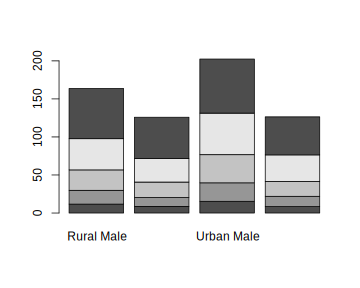
\includegraphics{Rprogramming_files/figure-latex/unnamed-chunk-8-5.png}

\begin{Shaded}
\begin{Highlighting}[]

\KeywordTok{barplot}\NormalTok{(VADeaths, }\DataTypeTok{col =} \KeywordTok{gray.colors}\NormalTok{(}\DecValTok{4}\NormalTok{), }\DataTypeTok{log=}\StringTok{"x"}\NormalTok{)}
\end{Highlighting}
\end{Shaded}

\includegraphics{Rprogramming_files/figure-latex/unnamed-chunk-8-6.png}

\begin{Shaded}
\begin{Highlighting}[]
\KeywordTok{barplot}\NormalTok{(VADeaths, }\DataTypeTok{col =} \KeywordTok{gray.colors}\NormalTok{(}\DecValTok{4}\NormalTok{), }\DataTypeTok{log=}\StringTok{"y"}\NormalTok{)}
\end{Highlighting}
\end{Shaded}

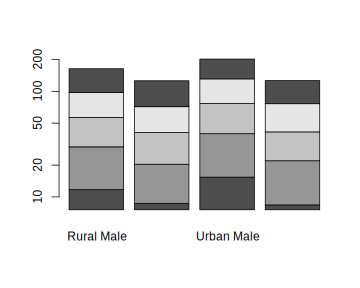
\includegraphics{Rprogramming_files/figure-latex/unnamed-chunk-8-7.png}

\begin{Shaded}
\begin{Highlighting}[]
\KeywordTok{barplot}\NormalTok{(VADeaths, }\DataTypeTok{col =} \KeywordTok{gray.colors}\NormalTok{(}\DecValTok{4}\NormalTok{), }\DataTypeTok{log=}\StringTok{"xy"}\NormalTok{)}
\end{Highlighting}
\end{Shaded}

\includegraphics{Rprogramming_files/figure-latex/unnamed-chunk-8-8.png}

\subsection{pie chart}\label{pie-chart}

\begin{Shaded}
\begin{Highlighting}[]
\NormalTok{drug.X.market <-}\StringTok{ }\KeywordTok{c}\NormalTok{(}\FloatTok{0.12}\NormalTok{, }\FloatTok{0.29}\NormalTok{, }\FloatTok{0.32}\NormalTok{, }\FloatTok{0.22}\NormalTok{, }\FloatTok{0.11}\NormalTok{, }\FloatTok{0.28}\NormalTok{)}
\KeywordTok{names}\NormalTok{(drug.X.market) <-}\StringTok{ }\KeywordTok{c}\NormalTok{(}\StringTok{"South Korea"}\NormalTok{,}\StringTok{"China"}\NormalTok{,}\StringTok{"USA"}\NormalTok{,}\StringTok{"Japan"}\NormalTok{,}\StringTok{"Austria"}\NormalTok{,}\StringTok{"EU"}\NormalTok{)}
\KeywordTok{pie}\NormalTok{(drug.X.market)}
\end{Highlighting}
\end{Shaded}

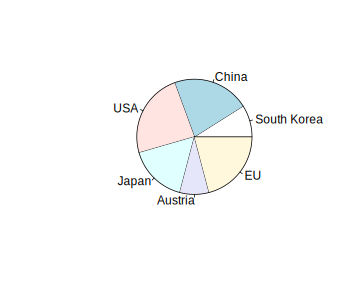
\includegraphics{Rprogramming_files/figure-latex/unnamed-chunk-9-1.png}

\subsection{matplot 함수}\label{matplot-}

\subsubsection{matrix와 column 사이의 그림}\label{matrix-column--}

\begin{Shaded}
\begin{Highlighting}[]
\NormalTok{pct.}\DecValTok{95}\NormalTok{ <-}\StringTok{ }\KeywordTok{read.csv}\NormalTok{(}\StringTok{"pct95.csv"}\NormalTok{)}
\KeywordTok{matplot}\NormalTok{(pct.}\DecValTok{95}\NormalTok{[,}\DecValTok{1}\NormalTok{], pct.}\DecValTok{95}\NormalTok{[,}\DecValTok{2}\OperatorTok{:}\KeywordTok{ncol}\NormalTok{(pct.}\DecValTok{95}\NormalTok{)], }\DataTypeTok{pch=}\DecValTok{1}\NormalTok{)}
\end{Highlighting}
\end{Shaded}

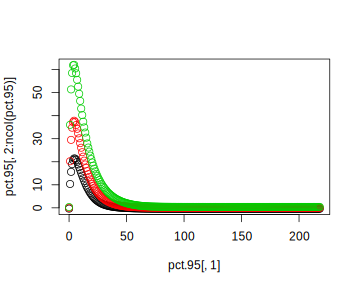
\includegraphics{Rprogramming_files/figure-latex/unnamed-chunk-10-1.png}

\begin{Shaded}
\begin{Highlighting}[]

\KeywordTok{matplot}\NormalTok{(pct.}\DecValTok{95}\NormalTok{[,}\DecValTok{1}\NormalTok{], pct.}\DecValTok{95}\NormalTok{[,}\DecValTok{2}\OperatorTok{:}\KeywordTok{ncol}\NormalTok{(pct.}\DecValTok{95}\NormalTok{)], }\DataTypeTok{pch=}\DecValTok{1}\NormalTok{, }\DataTypeTok{col=}\KeywordTok{c}\NormalTok{(}\DecValTok{1}\NormalTok{,}\DecValTok{2}\NormalTok{,}\DecValTok{1}\NormalTok{), }\DataTypeTok{type=}\StringTok{"l"}\NormalTok{, }\DataTypeTok{lty=}\DecValTok{1}\NormalTok{, }\DataTypeTok{lwd=}\KeywordTok{c}\NormalTok{(}\DecValTok{1}\NormalTok{,}\DecValTok{2}\NormalTok{,}\DecValTok{1}\NormalTok{))}
\end{Highlighting}
\end{Shaded}

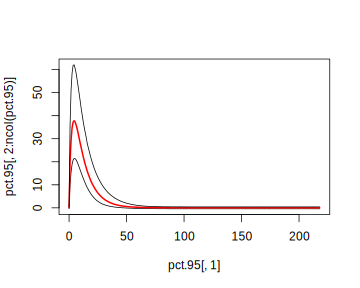
\includegraphics{Rprogramming_files/figure-latex/unnamed-chunk-10-2.png}

\subsection{Scatter plot matrices (pairs
plots)}\label{scatter-plot-matrices-pairs-plots}

\begin{Shaded}
\begin{Highlighting}[]
\KeywordTok{pairs}\NormalTok{(d.demog)}
\end{Highlighting}
\end{Shaded}

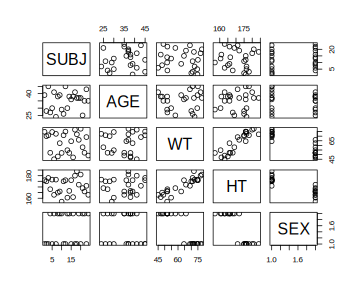
\includegraphics{Rprogramming_files/figure-latex/unnamed-chunk-11-1.png}

\subsubsection{add a loess smoother,
type}\label{add-a-loess-smoother-type}

\begin{Shaded}
\begin{Highlighting}[]
\KeywordTok{pairs}\NormalTok{(d.demog, }\DataTypeTok{panel =}\NormalTok{ panel.smooth)}
\end{Highlighting}
\end{Shaded}

\includegraphics{Rprogramming_files/figure-latex/unnamed-chunk-12-1.png}

\begin{Shaded}
\begin{Highlighting}[]

\NormalTok{panel.cor <-}\StringTok{ }\ControlFlowTok{function}\NormalTok{(x, y, }\DataTypeTok{digits=}\DecValTok{2}\NormalTok{, }\DataTypeTok{prefix=}\StringTok{""}\NormalTok{, cex.cor)}
\NormalTok{\{}
\NormalTok{    usr <-}\StringTok{ }\KeywordTok{par}\NormalTok{(}\StringTok{"usr"}\NormalTok{); }\KeywordTok{on.exit}\NormalTok{(}\KeywordTok{par}\NormalTok{(usr))}
    \KeywordTok{par}\NormalTok{(}\DataTypeTok{usr =} \KeywordTok{c}\NormalTok{(}\DecValTok{0}\NormalTok{, }\DecValTok{1}\NormalTok{, }\DecValTok{0}\NormalTok{, }\DecValTok{1}\NormalTok{))}
\NormalTok{    r =}\StringTok{ }\NormalTok{(}\KeywordTok{cor}\NormalTok{(x, y))}
\NormalTok{    txt <-}\StringTok{ }\KeywordTok{format}\NormalTok{(}\KeywordTok{c}\NormalTok{(r, }\FloatTok{0.123456789}\NormalTok{), }\DataTypeTok{digits=}\NormalTok{digits)[}\DecValTok{1}\NormalTok{]}
\NormalTok{    txt <-}\StringTok{ }\KeywordTok{paste}\NormalTok{(prefix, txt, }\DataTypeTok{sep=}\StringTok{""}\NormalTok{)}
    \ControlFlowTok{if}\NormalTok{(}\KeywordTok{missing}\NormalTok{(cex.cor)) cex <-}\StringTok{ }\FloatTok{1.5}
    \KeywordTok{text}\NormalTok{(}\FloatTok{0.5}\NormalTok{, }\FloatTok{0.5}\NormalTok{, txt, }\DataTypeTok{cex =} \FloatTok{1.5}\NormalTok{)}
\NormalTok{\}}

\KeywordTok{pairs}\NormalTok{(d.demog, }\DataTypeTok{lower.panel=}\NormalTok{panel.smooth, }\DataTypeTok{upper.panel=}\NormalTok{panel.cor) }
\end{Highlighting}
\end{Shaded}

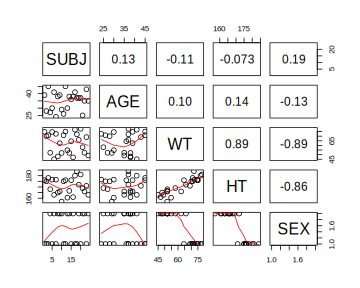
\includegraphics{Rprogramming_files/figure-latex/unnamed-chunk-12-2.png}

\section{하위수준 그림 함수}\label{lower}

\begin{itemize}
\tightlist
\item
  points : 점추가
\item
  lines : 선 추가
\item
  abline : 기준선 추가
\item
  mtext : 텍스트 추가
\item
  legend : 설명(legend) 추가
\item
  polygon : polygon 추가
\end{itemize}

\subsection{점, 선, 설명 추가 하기 \{add\}}\label{-----add}

\begin{Shaded}
\begin{Highlighting}[]
\KeywordTok{plot}\NormalTok{(pct.}\DecValTok{95}\OperatorTok{$}\NormalTok{TIME, pct.}\DecValTok{95}\OperatorTok{$}\NormalTok{PCT50, }\DataTypeTok{main=}\StringTok{"PK of Drug X"}
\NormalTok{     , }\DataTypeTok{type=}\StringTok{"l"}\NormalTok{, }\DataTypeTok{xlab=}\StringTok{"Time (h)"}\NormalTok{, }\DataTypeTok{ylab=}\StringTok{"Concentration (ng/ml)"}
\NormalTok{     , }\DataTypeTok{ylim=}\KeywordTok{range}\NormalTok{(}\DecValTok{0}\NormalTok{,}\DecValTok{80}\NormalTok{), }\DataTypeTok{lty=}\DecValTok{1}\NormalTok{, }\DataTypeTok{col=}\StringTok{"red"}\NormalTok{, }\DataTypeTok{lwd=}\DecValTok{2}\NormalTok{)}
\end{Highlighting}
\end{Shaded}

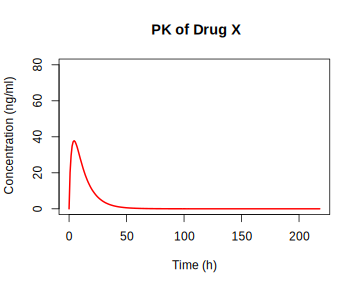
\includegraphics{Rprogramming_files/figure-latex/unnamed-chunk-13-1.png}

\begin{Shaded}
\begin{Highlighting}[]

\KeywordTok{plot}\NormalTok{(dta}\OperatorTok{$}\NormalTok{TIME[dta}\OperatorTok{$}\NormalTok{MDV}\OperatorTok{==}\DecValTok{0}\NormalTok{], dta}\OperatorTok{$}\NormalTok{DV[dta}\OperatorTok{$}\NormalTok{MDV}\OperatorTok{==}\DecValTok{0}\NormalTok{], }\DataTypeTok{main=}\StringTok{"PK of Drug X"}
\NormalTok{     , }\DataTypeTok{type=}\StringTok{"n"}\NormalTok{, }\DataTypeTok{xlab=}\StringTok{"Time (h)"}\NormalTok{, }\DataTypeTok{ylab=}\StringTok{"Concentration (ng/ml)"}
\NormalTok{     , }\DataTypeTok{ylim=}\KeywordTok{range}\NormalTok{(}\DecValTok{0}\NormalTok{,}\DecValTok{80}\NormalTok{))}
\KeywordTok{points}\NormalTok{(dta}\OperatorTok{$}\NormalTok{TIME[dta}\OperatorTok{$}\NormalTok{MDV}\OperatorTok{==}\DecValTok{0}\NormalTok{], dta}\OperatorTok{$}\NormalTok{DV[dta}\OperatorTok{$}\NormalTok{MDV}\OperatorTok{==}\DecValTok{0}\NormalTok{], }\DataTypeTok{pch =} \DecValTok{16}\NormalTok{, }\DataTypeTok{cex=}\FloatTok{0.8}\NormalTok{)}
\KeywordTok{lines}\NormalTok{(dta}\OperatorTok{$}\NormalTok{TIME[dta}\OperatorTok{$}\NormalTok{MDV}\OperatorTok{==}\DecValTok{0}\NormalTok{], dta}\OperatorTok{$}\NormalTok{DV[dta}\OperatorTok{$}\NormalTok{MDV}\OperatorTok{==}\DecValTok{0}\NormalTok{], }\DataTypeTok{col=}\StringTok{"black"}\NormalTok{, }\DataTypeTok{lwd=}\DecValTok{1}\NormalTok{)}
\KeywordTok{abline}\NormalTok{(}\DecValTok{40}\NormalTok{, }\DecValTok{0}\NormalTok{, }\DataTypeTok{col=}\StringTok{"red"}\NormalTok{, }\DataTypeTok{lty=}\DecValTok{2}\NormalTok{)                               }\CommentTok{# abline(a,b): y=a+b*x}
\KeywordTok{legend}\NormalTok{(}\StringTok{"topright"}\NormalTok{, }\DataTypeTok{legend=}\KeywordTok{c}\NormalTok{(}\StringTok{"Individual concentrations"}\NormalTok{)}
\NormalTok{       , }\DataTypeTok{lty=}\DecValTok{1}\NormalTok{, }\DataTypeTok{col=}\StringTok{"black"}\NormalTok{)}
\end{Highlighting}
\end{Shaded}

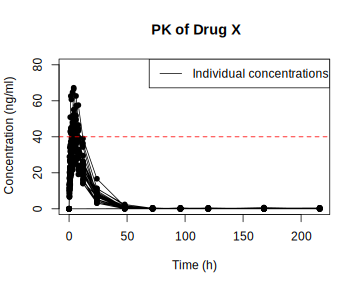
\includegraphics{Rprogramming_files/figure-latex/unnamed-chunk-13-2.png}

\subsection{polygon 함수}\label{polygon-}

\begin{Shaded}
\begin{Highlighting}[]
\KeywordTok{plot}\NormalTok{(}\KeywordTok{c}\NormalTok{(}\DecValTok{1}\NormalTok{, }\DecValTok{10}\NormalTok{), }\KeywordTok{c}\NormalTok{(}\DecValTok{1}\NormalTok{, }\DecValTok{6}\NormalTok{), }\DataTypeTok{type =} \StringTok{"n"}\NormalTok{)}
\KeywordTok{polygon}\NormalTok{(}\KeywordTok{c}\NormalTok{(}\DecValTok{2}\NormalTok{,}\DecValTok{8}\NormalTok{,}\DecValTok{8}\NormalTok{,}\DecValTok{2}\NormalTok{), }\KeywordTok{c}\NormalTok{(}\DecValTok{5}\NormalTok{,}\DecValTok{4}\NormalTok{,}\DecValTok{3}\NormalTok{,}\DecValTok{2}\NormalTok{), }\DataTypeTok{col=}\StringTok{"lightgreen"}\NormalTok{)}
\end{Highlighting}
\end{Shaded}

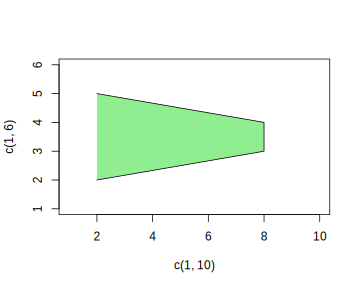
\includegraphics{Rprogramming_files/figure-latex/unnamed-chunk-14-1.png}

\begin{Shaded}
\begin{Highlighting}[]


\KeywordTok{plot}\NormalTok{(}\KeywordTok{c}\NormalTok{(}\DecValTok{1}\NormalTok{, }\DecValTok{9}\NormalTok{), }\DecValTok{1}\OperatorTok{:}\DecValTok{2}\NormalTok{, }\DataTypeTok{type =} \StringTok{"n"}\NormalTok{)}
\KeywordTok{polygon}\NormalTok{(}\DecValTok{1}\OperatorTok{:}\DecValTok{9}\NormalTok{, }\KeywordTok{c}\NormalTok{(}\DecValTok{2}\NormalTok{,}\DecValTok{1}\NormalTok{,}\DecValTok{2}\NormalTok{,}\DecValTok{1}\NormalTok{,}\DecValTok{1}\NormalTok{,}\DecValTok{2}\NormalTok{,}\DecValTok{1}\NormalTok{,}\DecValTok{2}\NormalTok{,}\DecValTok{1}\NormalTok{),}
        \DataTypeTok{col =} \KeywordTok{c}\NormalTok{(}\StringTok{"red"}\NormalTok{, }\StringTok{"blue"}\NormalTok{),}
        \DataTypeTok{border =} \KeywordTok{c}\NormalTok{(}\StringTok{"green"}\NormalTok{, }\StringTok{"yellow"}\NormalTok{),}
        \DataTypeTok{lwd =} \DecValTok{3}\NormalTok{, }\DataTypeTok{lty =} \KeywordTok{c}\NormalTok{(}\StringTok{"dashed"}\NormalTok{, }\StringTok{"solid"}\NormalTok{))}
\end{Highlighting}
\end{Shaded}

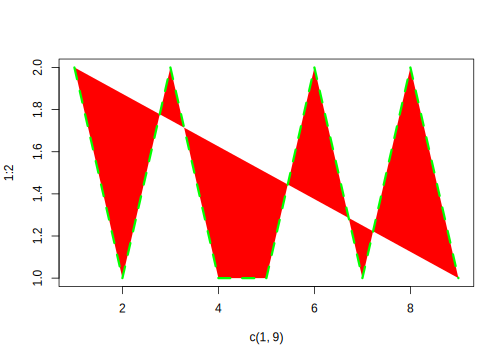
\includegraphics{Rprogramming_files/figure-latex/unnamed-chunk-14-2.png}

\section{그림 출력하기}\label{print}

\subsection{pdf graphics devices}\label{pdf-graphics-devices}

\begin{Shaded}
\begin{Highlighting}[]
\KeywordTok{pdf}\NormalTok{(}\StringTok{"PK_of_Drug_X.pdf"}\NormalTok{)}

\KeywordTok{plot}\NormalTok{(dta}\OperatorTok{$}\NormalTok{TIME[dta}\OperatorTok{$}\NormalTok{MDV}\OperatorTok{==}\DecValTok{0}\NormalTok{], dta}\OperatorTok{$}\NormalTok{DV[dta}\OperatorTok{$}\NormalTok{MDV}\OperatorTok{==}\DecValTok{0}\NormalTok{], }\DataTypeTok{main=}\StringTok{"PK of Drug X"}
\NormalTok{     , }\DataTypeTok{type=}\StringTok{"n"}\NormalTok{, }\DataTypeTok{xlab=}\StringTok{"Time (h)"}\NormalTok{, }\DataTypeTok{ylab=}\StringTok{"Concentration (ng/ml)"}
\NormalTok{     , }\DataTypeTok{ylim=}\KeywordTok{range}\NormalTok{(}\DecValTok{0}\NormalTok{,}\DecValTok{80}\NormalTok{))}
\KeywordTok{points}\NormalTok{(dta}\OperatorTok{$}\NormalTok{TIME[dta}\OperatorTok{$}\NormalTok{MDV}\OperatorTok{==}\DecValTok{0}\NormalTok{], dta}\OperatorTok{$}\NormalTok{DV[dta}\OperatorTok{$}\NormalTok{MDV}\OperatorTok{==}\DecValTok{0}\NormalTok{], }\DataTypeTok{pch =} \DecValTok{16}\NormalTok{, }\DataTypeTok{cex=}\FloatTok{0.8}\NormalTok{)}
\KeywordTok{lines}\NormalTok{(dta}\OperatorTok{$}\NormalTok{TIME[dta}\OperatorTok{$}\NormalTok{MDV}\OperatorTok{==}\DecValTok{0}\NormalTok{], dta}\OperatorTok{$}\NormalTok{DV[dta}\OperatorTok{$}\NormalTok{MDV}\OperatorTok{==}\DecValTok{0}\NormalTok{], }\DataTypeTok{col=}\StringTok{"black"}\NormalTok{, }\DataTypeTok{lwd=}\DecValTok{1}\NormalTok{)}
\KeywordTok{abline}\NormalTok{(}\DecValTok{40}\NormalTok{, }\DecValTok{0}\NormalTok{, }\DataTypeTok{col=}\StringTok{"red"}\NormalTok{, }\DataTypeTok{lty=}\DecValTok{2}\NormalTok{)                               }\CommentTok{#abline(a,b): y=a+b*x}
\KeywordTok{legend}\NormalTok{(}\StringTok{"topright"}\NormalTok{, }\DataTypeTok{legend=}\KeywordTok{c}\NormalTok{(}\StringTok{"Individual concentrations"}\NormalTok{)}
\NormalTok{       , }\DataTypeTok{lty=}\DecValTok{1}\NormalTok{, }\DataTypeTok{col=}\StringTok{"black"}\NormalTok{)}

\KeywordTok{dev.off}\NormalTok{()}
\NormalTok{## quartz_off_screen }
\NormalTok{##                 2}
\end{Highlighting}
\end{Shaded}

\subsection{PNG graphics devices}\label{png-graphics-devices}

\begin{Shaded}
\begin{Highlighting}[]
\KeywordTok{png}\NormalTok{(}\StringTok{"PK_of_Drug_X.png"}\NormalTok{)}

\KeywordTok{plot}\NormalTok{(dta}\OperatorTok{$}\NormalTok{TIME[dta}\OperatorTok{$}\NormalTok{MDV}\OperatorTok{==}\DecValTok{0}\NormalTok{], dta}\OperatorTok{$}\NormalTok{DV[dta}\OperatorTok{$}\NormalTok{MDV}\OperatorTok{==}\DecValTok{0}\NormalTok{], }\DataTypeTok{main=}\StringTok{"PK of Drug X"}
\NormalTok{     , }\DataTypeTok{type=}\StringTok{"n"}\NormalTok{, }\DataTypeTok{xlab=}\StringTok{"Time (h)"}\NormalTok{, }\DataTypeTok{ylab=}\StringTok{"Concentration (ng/ml)"}
\NormalTok{     , }\DataTypeTok{ylim=}\KeywordTok{range}\NormalTok{(}\DecValTok{0}\NormalTok{,}\DecValTok{80}\NormalTok{))}
\KeywordTok{points}\NormalTok{(dta}\OperatorTok{$}\NormalTok{TIME[dta}\OperatorTok{$}\NormalTok{MDV}\OperatorTok{==}\DecValTok{0}\NormalTok{], dta}\OperatorTok{$}\NormalTok{DV[dta}\OperatorTok{$}\NormalTok{MDV}\OperatorTok{==}\DecValTok{0}\NormalTok{], }\DataTypeTok{pch =} \DecValTok{16}\NormalTok{, }\DataTypeTok{cex=}\FloatTok{0.8}\NormalTok{)}
\KeywordTok{lines}\NormalTok{(dta}\OperatorTok{$}\NormalTok{TIME[dta}\OperatorTok{$}\NormalTok{MDV}\OperatorTok{==}\DecValTok{0}\NormalTok{], dta}\OperatorTok{$}\NormalTok{DV[dta}\OperatorTok{$}\NormalTok{MDV}\OperatorTok{==}\DecValTok{0}\NormalTok{], }\DataTypeTok{col=}\StringTok{"black"}\NormalTok{, }\DataTypeTok{lwd=}\DecValTok{1}\NormalTok{)}
\KeywordTok{abline}\NormalTok{(}\DecValTok{40}\NormalTok{, }\DecValTok{0}\NormalTok{, }\DataTypeTok{col=}\StringTok{"red"}\NormalTok{, }\DataTypeTok{lty=}\DecValTok{2}\NormalTok{)                               }\CommentTok{#abline(a,b): y=a+b*x}
\KeywordTok{legend}\NormalTok{(}\StringTok{"topright"}\NormalTok{, }\DataTypeTok{legend=}\KeywordTok{c}\NormalTok{(}\StringTok{"Individual concentrations"}\NormalTok{)}
\NormalTok{       , }\DataTypeTok{lty=}\DecValTok{1}\NormalTok{, }\DataTypeTok{col=}\StringTok{"black"}\NormalTok{)}

\KeywordTok{dev.off}\NormalTok{()}
\NormalTok{## quartz_off_screen }
\NormalTok{##                 2}
\end{Highlighting}
\end{Shaded}

\chapter{Data Import / Export}\label{data-import-export}

\begin{quote}
2017-03-29 배균섭 교수님 강의
\end{quote}

이번 시간에는 자료를 불러오고 조작을 가한 뒤 저장하는 방법에 대해
알아보겠습니다.

\section{Read.csv}\label{read.csv}

\texttt{setwd} 명령어를 통해서 자료가 있는 작업 공간을 설정할 수
있습니다. 설정 후에서는 \texttt{dir()}을 통해 파일의 이름을 확인 할 수
있습니다. \texttt{read.csv}를 통해서 자료를 R에서 사용할 수 있게 됩니다.

\begin{Shaded}
\begin{Highlighting}[]
\KeywordTok{setwd}\NormalTok{(}\StringTok{"D:/Rt"}\NormalTok{)}
\KeywordTok{dir}\NormalTok{()}
\NormalTok{mydata <-}\StringTok{ }\KeywordTok{read.csv}\NormalTok{(}\StringTok{"MyData2017.csv"}\NormalTok{, }\DataTypeTok{as.is=}\OtherTok{TRUE}\NormalTok{)}
\end{Highlighting}
\end{Shaded}

\section{Theoph 데이타}\label{theoph-}

R에 기본적으로 들어있는 \texttt{Theoph} 약동학 자료에 대해
살펴보겠습니다.

\begin{Shaded}
\begin{Highlighting}[]
\KeywordTok{head}\NormalTok{(Theoph, }\DataTypeTok{n =} \DecValTok{11}\NormalTok{)}
\NormalTok{##    Subject   Wt Dose  Time  conc}
\NormalTok{## 1        1 79.6 4.02  0.00  0.74}
\NormalTok{## 2        1 79.6 4.02  0.25  2.84}
\NormalTok{## 3        1 79.6 4.02  0.57  6.57}
\NormalTok{## 4        1 79.6 4.02  1.12 10.50}
\NormalTok{## 5        1 79.6 4.02  2.02  9.66}
\NormalTok{## 6        1 79.6 4.02  3.82  8.58}
\NormalTok{## 7        1 79.6 4.02  5.10  8.36}
\NormalTok{## 8        1 79.6 4.02  7.03  7.47}
\NormalTok{## 9        1 79.6 4.02  9.05  6.89}
\NormalTok{## 10       1 79.6 4.02 12.12  5.94}
\NormalTok{## 11       1 79.6 4.02 24.37  3.28}
\KeywordTok{tail}\NormalTok{(Theoph, }\DataTypeTok{n =} \DecValTok{11}\NormalTok{)}
\NormalTok{##     Subject   Wt Dose  Time conc}
\NormalTok{## 122      12 60.5  5.3  0.00 0.00}
\NormalTok{## 123      12 60.5  5.3  0.25 1.25}
\NormalTok{## 124      12 60.5  5.3  0.50 3.96}
\NormalTok{## 125      12 60.5  5.3  1.00 7.82}
\NormalTok{## 126      12 60.5  5.3  2.00 9.72}
\NormalTok{## 127      12 60.5  5.3  3.52 9.75}
\NormalTok{## 128      12 60.5  5.3  5.07 8.57}
\NormalTok{## 129      12 60.5  5.3  7.07 6.59}
\NormalTok{## 130      12 60.5  5.3  9.03 6.11}
\NormalTok{## 131      12 60.5  5.3 12.05 4.57}
\NormalTok{## 132      12 60.5  5.3 24.15 1.17}
\end{Highlighting}
\end{Shaded}

R console에서 \texttt{?Theoph}를 타이핑 치면 좀 더 자세한 정보를 얻을 수
있습니다.

\section{lattice}\label{lattice}

lattice 패키지를 불러온 뒤 그림을 그려보겠습니다. \citep{R-lattice}
\index{lattice}

\begin{Shaded}
\begin{Highlighting}[]
\KeywordTok{library}\NormalTok{(lattice) }\CommentTok{# trellis}

\KeywordTok{xyplot}\NormalTok{(conc }\OperatorTok{~}\StringTok{ }\NormalTok{Time }\OperatorTok{|}\StringTok{ }\NormalTok{Subject, }\DataTypeTok{data=}\NormalTok{Theoph)}
\end{Highlighting}
\end{Shaded}

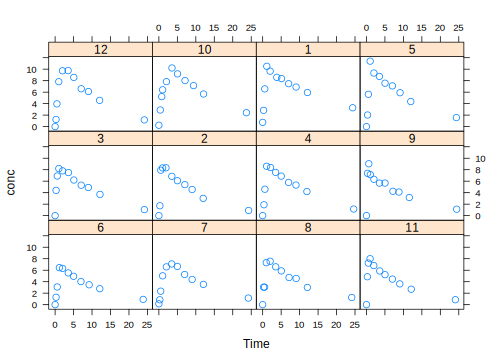
\includegraphics{Rprogramming_files/figure-latex/unnamed-chunk-19-1.png}

\begin{Shaded}
\begin{Highlighting}[]

\KeywordTok{xyplot}\NormalTok{(conc }\OperatorTok{~}\StringTok{ }\NormalTok{Time }\OperatorTok{|}\StringTok{ }\NormalTok{Subject, }\DataTypeTok{data=}\NormalTok{Theoph, }\DataTypeTok{type=}\StringTok{"b"}\NormalTok{)}
\end{Highlighting}
\end{Shaded}

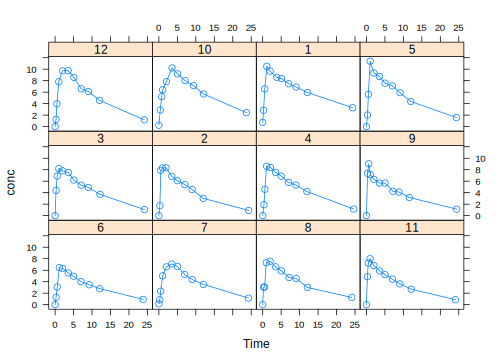
\includegraphics{Rprogramming_files/figure-latex/unnamed-chunk-19-2.png}

\begin{Shaded}
\begin{Highlighting}[]

\NormalTok{Theoph[,}\StringTok{"ID"}\NormalTok{] =}\StringTok{ }\KeywordTok{as.numeric}\NormalTok{(}\KeywordTok{as.character}\NormalTok{(Theoph[,}\StringTok{"Subject"}\NormalTok{]))}

\KeywordTok{xyplot}\NormalTok{(conc }\OperatorTok{~}\StringTok{ }\NormalTok{Time }\OperatorTok{|}\StringTok{ }\NormalTok{ID, }\DataTypeTok{data=}\NormalTok{Theoph, }\DataTypeTok{type=}\StringTok{"b"}\NormalTok{)}
\end{Highlighting}
\end{Shaded}

\includegraphics{Rprogramming_files/figure-latex/unnamed-chunk-19-3.png}

\begin{Shaded}
\begin{Highlighting}[]

\KeywordTok{xyplot}\NormalTok{(conc }\OperatorTok{~}\StringTok{ }\NormalTok{Time }\OperatorTok{|}\StringTok{ }\KeywordTok{as.factor}\NormalTok{(ID), }\DataTypeTok{data=}\NormalTok{Theoph, }\DataTypeTok{type=}\StringTok{"b"}\NormalTok{)}
\end{Highlighting}
\end{Shaded}

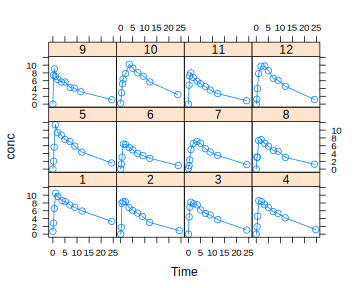
\includegraphics{Rprogramming_files/figure-latex/unnamed-chunk-19-4.png}

\begin{Shaded}
\begin{Highlighting}[]

\KeywordTok{write.csv}\NormalTok{(Theoph, }\StringTok{"Theoph.csv"}\NormalTok{, }\DataTypeTok{row.names=}\OtherTok{FALSE}\NormalTok{, }\DataTypeTok{quote=}\OtherTok{FALSE}\NormalTok{, }\DataTypeTok{na=}\StringTok{""}\NormalTok{)}
\end{Highlighting}
\end{Shaded}

\section{Subseting and write.csv}\label{subseting-and-write.csv}

자료를 편집하고, subset을 만들고 각각을 파일로 저장하는 방법에 대해
알아보겠습니다.

\begin{Shaded}
\begin{Highlighting}[]
\NormalTok{IDs =}\StringTok{ }\KeywordTok{sort}\NormalTok{(}\KeywordTok{unique}\NormalTok{(Theoph[,}\StringTok{"ID"}\NormalTok{])) ; IDs}
\NormalTok{##  [1]  1  2  3  4  5  6  7  8  9 10 11 12}
\NormalTok{nID =}\StringTok{ }\KeywordTok{length}\NormalTok{(IDs) ; nID}
\NormalTok{## [1] 12}

\NormalTok{demog =}\StringTok{ }\KeywordTok{unique}\NormalTok{(Theoph[,}\KeywordTok{c}\NormalTok{(}\StringTok{"ID"}\NormalTok{,}\StringTok{"Wt"}\NormalTok{)])}
\KeywordTok{colnames}\NormalTok{(demog) =}\StringTok{ }\KeywordTok{c}\NormalTok{(}\StringTok{"ID"}\NormalTok{, }\StringTok{"BWT"}\NormalTok{)}
\KeywordTok{write.csv}\NormalTok{(demog, }\StringTok{"1-demog.csv"}\NormalTok{, }\DataTypeTok{row.names=}\OtherTok{FALSE}\NormalTok{, }\DataTypeTok{quote=}\OtherTok{FALSE}\NormalTok{, }\DataTypeTok{na=}\StringTok{""}\NormalTok{)}

\NormalTok{DV =}\StringTok{ }\NormalTok{Theoph[,}\KeywordTok{c}\NormalTok{(}\StringTok{"ID"}\NormalTok{,}\StringTok{"Time"}\NormalTok{, }\StringTok{"conc"}\NormalTok{)]}
\KeywordTok{colnames}\NormalTok{(DV) =}\StringTok{ }\KeywordTok{c}\NormalTok{(}\StringTok{"ID"}\NormalTok{, }\StringTok{"TIME"}\NormalTok{, }\StringTok{"DV"}\NormalTok{)}
\KeywordTok{write.csv}\NormalTok{(DV, }\StringTok{"3-DV.csv"}\NormalTok{, }\DataTypeTok{row.names=}\OtherTok{FALSE}\NormalTok{, }\DataTypeTok{quote=}\OtherTok{FALSE}\NormalTok{, }\DataTypeTok{na=}\StringTok{""}\NormalTok{)}

\NormalTok{adm =}\StringTok{ }\KeywordTok{cbind}\NormalTok{(IDs, }\KeywordTok{rep}\NormalTok{(}\DecValTok{0}\NormalTok{, nID), }\KeywordTok{rep}\NormalTok{(}\DecValTok{320}\NormalTok{, nID))}
\KeywordTok{colnames}\NormalTok{(adm) =}\StringTok{ }\KeywordTok{c}\NormalTok{(}\StringTok{"ID"}\NormalTok{, }\StringTok{"TIME"}\NormalTok{, }\StringTok{"AMT"}\NormalTok{)}
\KeywordTok{write.csv}\NormalTok{(adm, }\StringTok{"2-adm.csv"}\NormalTok{, }\DataTypeTok{row.names=}\OtherTok{FALSE}\NormalTok{, }\DataTypeTok{quote=}\OtherTok{FALSE}\NormalTok{, }\DataTypeTok{na=}\StringTok{""}\NormalTok{)}

\NormalTok{demog =}\StringTok{ }\KeywordTok{read.csv}\NormalTok{(}\StringTok{"1-demog.csv"}\NormalTok{, }\DataTypeTok{as.is=}\OtherTok{TRUE}\NormalTok{)}
\NormalTok{adm =}\StringTok{ }\KeywordTok{read.csv}\NormalTok{(}\StringTok{"2-adm.csv"}\NormalTok{, }\DataTypeTok{as.is=}\OtherTok{TRUE}\NormalTok{)}
\NormalTok{dv =}\StringTok{ }\KeywordTok{read.csv}\NormalTok{(}\StringTok{"3-dv.csv"}\NormalTok{, }\DataTypeTok{as.is=}\OtherTok{TRUE}\NormalTok{)}

\NormalTok{AdmDv =}\StringTok{ }\KeywordTok{merge}\NormalTok{(adm, dv, }\DataTypeTok{by=}\KeywordTok{intersect}\NormalTok{(}\KeywordTok{colnames}\NormalTok{(adm), }\KeywordTok{colnames}\NormalTok{(dv)), }\DataTypeTok{all=}\OtherTok{TRUE}\NormalTok{)}
\NormalTok{AdmDv}
\NormalTok{##     ID  TIME AMT    DV}
\NormalTok{## 1    1  0.00 320  0.74}
\NormalTok{## 2    1  0.25  NA  2.84}
\NormalTok{## 3    1  0.57  NA  6.57}
\NormalTok{## 4    1  1.12  NA 10.50}
\NormalTok{## 5    1  2.02  NA  9.66}
\NormalTok{## 6    1  3.82  NA  8.58}
\NormalTok{## 7    1  5.10  NA  8.36}
\NormalTok{## 8    1  7.03  NA  7.47}
\NormalTok{## 9    1  9.05  NA  6.89}
\NormalTok{## 10   1 12.12  NA  5.94}
\NormalTok{## 11   1 24.37  NA  3.28}
\NormalTok{## 12   2  0.00 320  0.00}
\NormalTok{## 13   2  0.27  NA  1.72}
\NormalTok{## 14   2  0.52  NA  7.91}
\NormalTok{## 15   2  1.00  NA  8.31}
\NormalTok{## 16   2  1.92  NA  8.33}
\NormalTok{## 17   2  3.50  NA  6.85}
\NormalTok{## 18   2  5.02  NA  6.08}
\NormalTok{## 19   2  7.03  NA  5.40}
\NormalTok{## 20   2  9.00  NA  4.55}
\NormalTok{## 21   2 12.00  NA  3.01}
\NormalTok{## 22   2 24.30  NA  0.90}
\NormalTok{## 23   3  0.00 320  0.00}
\NormalTok{## 24   3  0.27  NA  4.40}
\NormalTok{## 25   3  0.58  NA  6.90}
\NormalTok{## 26   3  1.02  NA  8.20}
\NormalTok{## 27   3  2.02  NA  7.80}
\NormalTok{## 28   3  3.62  NA  7.50}
\NormalTok{## 29   3  5.08  NA  6.20}
\NormalTok{## 30   3  7.07  NA  5.30}
\NormalTok{## 31   3  9.00  NA  4.90}
\NormalTok{## 32   3 12.15  NA  3.70}
\NormalTok{## 33   3 24.17  NA  1.05}
\NormalTok{## 34   4  0.00 320  0.00}
\NormalTok{## 35   4  0.35  NA  1.89}
\NormalTok{## 36   4  0.60  NA  4.60}
\NormalTok{## 37   4  1.07  NA  8.60}
\NormalTok{## 38   4  2.13  NA  8.38}
\NormalTok{## 39   4  3.50  NA  7.54}
\NormalTok{## 40   4  5.02  NA  6.88}
\NormalTok{## 41   4  7.02  NA  5.78}
\NormalTok{## 42   4  9.02  NA  5.33}
\NormalTok{## 43   4 11.98  NA  4.19}
\NormalTok{## 44   4 24.65  NA  1.15}
\NormalTok{## 45   5  0.00 320  0.00}
\NormalTok{## 46   5  0.30  NA  2.02}
\NormalTok{## 47   5  0.52  NA  5.63}
\NormalTok{## 48   5  1.00  NA 11.40}
\NormalTok{## 49   5  2.02  NA  9.33}
\NormalTok{## 50   5  3.50  NA  8.74}
\NormalTok{## 51   5  5.02  NA  7.56}
\NormalTok{## 52   5  7.02  NA  7.09}
\NormalTok{## 53   5  9.10  NA  5.90}
\NormalTok{## 54   5 12.00  NA  4.37}
\NormalTok{## 55   5 24.35  NA  1.57}
\NormalTok{## 56   6  0.00 320  0.00}
\NormalTok{## 57   6  0.27  NA  1.29}
\NormalTok{## 58   6  0.58  NA  3.08}
\NormalTok{## 59   6  1.15  NA  6.44}
\NormalTok{## 60   6  2.03  NA  6.32}
\NormalTok{## 61   6  3.57  NA  5.53}
\NormalTok{## 62   6  5.00  NA  4.94}
\NormalTok{## 63   6  7.00  NA  4.02}
\NormalTok{## 64   6  9.22  NA  3.46}
\NormalTok{## 65   6 12.10  NA  2.78}
\NormalTok{## 66   6 23.85  NA  0.92}
\NormalTok{## 67   7  0.00 320  0.15}
\NormalTok{## 68   7  0.25  NA  0.85}
\NormalTok{## 69   7  0.50  NA  2.35}
\NormalTok{## 70   7  1.02  NA  5.02}
\NormalTok{## 71   7  2.02  NA  6.58}
\NormalTok{## 72   7  3.48  NA  7.09}
\NormalTok{## 73   7  5.00  NA  6.66}
\NormalTok{## 74   7  6.98  NA  5.25}
\NormalTok{## 75   7  9.00  NA  4.39}
\NormalTok{## 76   7 12.05  NA  3.53}
\NormalTok{## 77   7 24.22  NA  1.15}
\NormalTok{## 78   8  0.00 320  0.00}
\NormalTok{## 79   8  0.25  NA  3.05}
\NormalTok{## 80   8  0.52  NA  3.05}
\NormalTok{## 81   8  0.98  NA  7.31}
\NormalTok{## 82   8  2.02  NA  7.56}
\NormalTok{## 83   8  3.53  NA  6.59}
\NormalTok{## 84   8  5.05  NA  5.88}
\NormalTok{## 85   8  7.15  NA  4.73}
\NormalTok{## 86   8  9.07  NA  4.57}
\NormalTok{## 87   8 12.10  NA  3.00}
\NormalTok{## 88   8 24.12  NA  1.25}
\NormalTok{## 89   9  0.00 320  0.00}
\NormalTok{## 90   9  0.30  NA  7.37}
\NormalTok{## 91   9  0.63  NA  9.03}
\NormalTok{## 92   9  1.05  NA  7.14}
\NormalTok{## 93   9  2.02  NA  6.33}
\NormalTok{## 94   9  3.53  NA  5.66}
\NormalTok{## 95   9  5.02  NA  5.67}
\NormalTok{## 96   9  7.17  NA  4.24}
\NormalTok{## 97   9  8.80  NA  4.11}
\NormalTok{## 98   9 11.60  NA  3.16}
\NormalTok{## 99   9 24.43  NA  1.12}
\NormalTok{## 100 10  0.00 320  0.24}
\NormalTok{## 101 10  0.37  NA  2.89}
\NormalTok{## 102 10  0.77  NA  5.22}
\NormalTok{## 103 10  1.02  NA  6.41}
\NormalTok{## 104 10  2.05  NA  7.83}
\NormalTok{## 105 10  3.55  NA 10.21}
\NormalTok{## 106 10  5.05  NA  9.18}
\NormalTok{## 107 10  7.08  NA  8.02}
\NormalTok{## 108 10  9.38  NA  7.14}
\NormalTok{## 109 10 12.10  NA  5.68}
\NormalTok{## 110 10 23.70  NA  2.42}
\NormalTok{## 111 11  0.00 320  0.00}
\NormalTok{## 112 11  0.25  NA  4.86}
\NormalTok{## 113 11  0.50  NA  7.24}
\NormalTok{## 114 11  0.98  NA  8.00}
\NormalTok{## 115 11  1.98  NA  6.81}
\NormalTok{## 116 11  3.60  NA  5.87}
\NormalTok{## 117 11  5.02  NA  5.22}
\NormalTok{## 118 11  7.03  NA  4.45}
\NormalTok{## 119 11  9.03  NA  3.62}
\NormalTok{## 120 11 12.12  NA  2.69}
\NormalTok{## 121 11 24.08  NA  0.86}
\NormalTok{## 122 12  0.00 320  0.00}
\NormalTok{## 123 12  0.25  NA  1.25}
\NormalTok{## 124 12  0.50  NA  3.96}
\NormalTok{## 125 12  1.00  NA  7.82}
\NormalTok{## 126 12  2.00  NA  9.72}
\NormalTok{## 127 12  3.52  NA  9.75}
\NormalTok{## 128 12  5.07  NA  8.57}
\NormalTok{## 129 12  7.07  NA  6.59}
\NormalTok{## 130 12  9.03  NA  6.11}
\NormalTok{## 131 12 12.05  NA  4.57}
\NormalTok{## 132 12 24.15  NA  1.17}
\end{Highlighting}
\end{Shaded}

자료를 병합(\texttt{merge})해 보겠습니다.

\begin{Shaded}
\begin{Highlighting}[]
\NormalTok{DataAll =}\StringTok{ }\KeywordTok{merge}\NormalTok{(demog, AdmDv, }\DataTypeTok{by=}\KeywordTok{c}\NormalTok{(}\StringTok{"ID"}\NormalTok{), }\DataTypeTok{all=}\OtherTok{TRUE}\NormalTok{)}
\NormalTok{DataAll}
\NormalTok{##     ID  BWT  TIME AMT    DV}
\NormalTok{## 1    1 79.6  0.00 320  0.74}
\NormalTok{## 2    1 79.6  0.25  NA  2.84}
\NormalTok{## 3    1 79.6  0.57  NA  6.57}
\NormalTok{## 4    1 79.6  1.12  NA 10.50}
\NormalTok{## 5    1 79.6  2.02  NA  9.66}
\NormalTok{## 6    1 79.6  3.82  NA  8.58}
\NormalTok{## 7    1 79.6  5.10  NA  8.36}
\NormalTok{## 8    1 79.6  7.03  NA  7.47}
\NormalTok{## 9    1 79.6  9.05  NA  6.89}
\NormalTok{## 10   1 79.6 12.12  NA  5.94}
\NormalTok{## 11   1 79.6 24.37  NA  3.28}
\NormalTok{## 12   2 72.4  0.00 320  0.00}
\NormalTok{## 13   2 72.4  0.27  NA  1.72}
\NormalTok{## 14   2 72.4  0.52  NA  7.91}
\NormalTok{## 15   2 72.4  1.00  NA  8.31}
\NormalTok{## 16   2 72.4  1.92  NA  8.33}
\NormalTok{## 17   2 72.4  3.50  NA  6.85}
\NormalTok{## 18   2 72.4  5.02  NA  6.08}
\NormalTok{## 19   2 72.4  7.03  NA  5.40}
\NormalTok{## 20   2 72.4  9.00  NA  4.55}
\NormalTok{## 21   2 72.4 12.00  NA  3.01}
\NormalTok{## 22   2 72.4 24.30  NA  0.90}
\NormalTok{## 23   3 70.5  0.00 320  0.00}
\NormalTok{## 24   3 70.5  0.27  NA  4.40}
\NormalTok{## 25   3 70.5  0.58  NA  6.90}
\NormalTok{## 26   3 70.5  1.02  NA  8.20}
\NormalTok{## 27   3 70.5  2.02  NA  7.80}
\NormalTok{## 28   3 70.5  3.62  NA  7.50}
\NormalTok{## 29   3 70.5  5.08  NA  6.20}
\NormalTok{## 30   3 70.5  7.07  NA  5.30}
\NormalTok{## 31   3 70.5  9.00  NA  4.90}
\NormalTok{## 32   3 70.5 12.15  NA  3.70}
\NormalTok{## 33   3 70.5 24.17  NA  1.05}
\NormalTok{## 34   4 72.7  0.00 320  0.00}
\NormalTok{## 35   4 72.7  0.35  NA  1.89}
\NormalTok{## 36   4 72.7  0.60  NA  4.60}
\NormalTok{## 37   4 72.7  1.07  NA  8.60}
\NormalTok{## 38   4 72.7  2.13  NA  8.38}
\NormalTok{## 39   4 72.7  3.50  NA  7.54}
\NormalTok{## 40   4 72.7  5.02  NA  6.88}
\NormalTok{## 41   4 72.7  7.02  NA  5.78}
\NormalTok{## 42   4 72.7  9.02  NA  5.33}
\NormalTok{## 43   4 72.7 11.98  NA  4.19}
\NormalTok{## 44   4 72.7 24.65  NA  1.15}
\NormalTok{## 45   5 54.6  0.00 320  0.00}
\NormalTok{## 46   5 54.6  0.30  NA  2.02}
\NormalTok{## 47   5 54.6  0.52  NA  5.63}
\NormalTok{## 48   5 54.6  1.00  NA 11.40}
\NormalTok{## 49   5 54.6  2.02  NA  9.33}
\NormalTok{## 50   5 54.6  3.50  NA  8.74}
\NormalTok{## 51   5 54.6  5.02  NA  7.56}
\NormalTok{## 52   5 54.6  7.02  NA  7.09}
\NormalTok{## 53   5 54.6  9.10  NA  5.90}
\NormalTok{## 54   5 54.6 12.00  NA  4.37}
\NormalTok{## 55   5 54.6 24.35  NA  1.57}
\NormalTok{## 56   6 80.0  0.00 320  0.00}
\NormalTok{## 57   6 80.0  0.27  NA  1.29}
\NormalTok{## 58   6 80.0  0.58  NA  3.08}
\NormalTok{## 59   6 80.0  1.15  NA  6.44}
\NormalTok{## 60   6 80.0  2.03  NA  6.32}
\NormalTok{## 61   6 80.0  3.57  NA  5.53}
\NormalTok{## 62   6 80.0  5.00  NA  4.94}
\NormalTok{## 63   6 80.0  7.00  NA  4.02}
\NormalTok{## 64   6 80.0  9.22  NA  3.46}
\NormalTok{## 65   6 80.0 12.10  NA  2.78}
\NormalTok{## 66   6 80.0 23.85  NA  0.92}
\NormalTok{## 67   7 64.6  0.00 320  0.15}
\NormalTok{## 68   7 64.6  0.25  NA  0.85}
\NormalTok{## 69   7 64.6  0.50  NA  2.35}
\NormalTok{## 70   7 64.6  1.02  NA  5.02}
\NormalTok{## 71   7 64.6  2.02  NA  6.58}
\NormalTok{## 72   7 64.6  3.48  NA  7.09}
\NormalTok{## 73   7 64.6  5.00  NA  6.66}
\NormalTok{## 74   7 64.6  6.98  NA  5.25}
\NormalTok{## 75   7 64.6  9.00  NA  4.39}
\NormalTok{## 76   7 64.6 12.05  NA  3.53}
\NormalTok{## 77   7 64.6 24.22  NA  1.15}
\NormalTok{## 78   8 70.5  0.00 320  0.00}
\NormalTok{## 79   8 70.5  0.25  NA  3.05}
\NormalTok{## 80   8 70.5  0.52  NA  3.05}
\NormalTok{## 81   8 70.5  0.98  NA  7.31}
\NormalTok{## 82   8 70.5  2.02  NA  7.56}
\NormalTok{## 83   8 70.5  3.53  NA  6.59}
\NormalTok{## 84   8 70.5  5.05  NA  5.88}
\NormalTok{## 85   8 70.5  7.15  NA  4.73}
\NormalTok{## 86   8 70.5  9.07  NA  4.57}
\NormalTok{## 87   8 70.5 12.10  NA  3.00}
\NormalTok{## 88   8 70.5 24.12  NA  1.25}
\NormalTok{## 89   9 86.4  0.00 320  0.00}
\NormalTok{## 90   9 86.4  0.30  NA  7.37}
\NormalTok{## 91   9 86.4  0.63  NA  9.03}
\NormalTok{## 92   9 86.4  1.05  NA  7.14}
\NormalTok{## 93   9 86.4  2.02  NA  6.33}
\NormalTok{## 94   9 86.4  3.53  NA  5.66}
\NormalTok{## 95   9 86.4  5.02  NA  5.67}
\NormalTok{## 96   9 86.4  7.17  NA  4.24}
\NormalTok{## 97   9 86.4  8.80  NA  4.11}
\NormalTok{## 98   9 86.4 11.60  NA  3.16}
\NormalTok{## 99   9 86.4 24.43  NA  1.12}
\NormalTok{## 100 10 58.2  0.00 320  0.24}
\NormalTok{## 101 10 58.2  0.37  NA  2.89}
\NormalTok{## 102 10 58.2  0.77  NA  5.22}
\NormalTok{## 103 10 58.2  1.02  NA  6.41}
\NormalTok{## 104 10 58.2  2.05  NA  7.83}
\NormalTok{## 105 10 58.2  3.55  NA 10.21}
\NormalTok{## 106 10 58.2  5.05  NA  9.18}
\NormalTok{## 107 10 58.2  7.08  NA  8.02}
\NormalTok{## 108 10 58.2  9.38  NA  7.14}
\NormalTok{## 109 10 58.2 12.10  NA  5.68}
\NormalTok{## 110 10 58.2 23.70  NA  2.42}
\NormalTok{## 111 11 65.0  0.00 320  0.00}
\NormalTok{## 112 11 65.0  0.25  NA  4.86}
\NormalTok{## 113 11 65.0  0.50  NA  7.24}
\NormalTok{## 114 11 65.0  0.98  NA  8.00}
\NormalTok{## 115 11 65.0  1.98  NA  6.81}
\NormalTok{## 116 11 65.0  3.60  NA  5.87}
\NormalTok{## 117 11 65.0  5.02  NA  5.22}
\NormalTok{## 118 11 65.0  7.03  NA  4.45}
\NormalTok{## 119 11 65.0  9.03  NA  3.62}
\NormalTok{## 120 11 65.0 12.12  NA  2.69}
\NormalTok{## 121 11 65.0 24.08  NA  0.86}
\NormalTok{## 122 12 60.5  0.00 320  0.00}
\NormalTok{## 123 12 60.5  0.25  NA  1.25}
\NormalTok{## 124 12 60.5  0.50  NA  3.96}
\NormalTok{## 125 12 60.5  1.00  NA  7.82}
\NormalTok{## 126 12 60.5  2.00  NA  9.72}
\NormalTok{## 127 12 60.5  3.52  NA  9.75}
\NormalTok{## 128 12 60.5  5.07  NA  8.57}
\NormalTok{## 129 12 60.5  7.07  NA  6.59}
\NormalTok{## 130 12 60.5  9.03  NA  6.11}
\NormalTok{## 131 12 60.5 12.05  NA  4.57}
\NormalTok{## 132 12 60.5 24.15  NA  1.17}
\end{Highlighting}
\end{Shaded}

\chapter{Frequently Used Functions}\label{frequently-used-functions}

\begin{quote}
2017-04-05 배균섭 교수님 강의
\end{quote}

자주 쓰는 함수 및 명령어에 대해 알아보겠습니다.

\section{Command}\label{command}

\begin{Shaded}
\begin{Highlighting}[]

\CommentTok{# 2017-04-05 R-intro.pdf Chapter 08}

\NormalTok{pois}
\CommentTok{# ?dbeta}
\KeywordTok{dnorm}\NormalTok{(}\DecValTok{0}\NormalTok{)}
\KeywordTok{pnorm}\NormalTok{(}\DecValTok{0}\NormalTok{)}
\DecValTok{1} \OperatorTok{-}\StringTok{ }\KeywordTok{pnorm}\NormalTok{(}\FloatTok{1.96}\NormalTok{)}
\CommentTok{# ?pnorm}
\KeywordTok{pnorm}\NormalTok{(}\FloatTok{1.96}\NormalTok{, }\DataTypeTok{lower.tail=}\OtherTok{FALSE}\NormalTok{)}
\KeywordTok{qnorm}\NormalTok{(}\FloatTok{0.5}\NormalTok{)}
\KeywordTok{qnorm}\NormalTok{(}\FloatTok{0.975}\NormalTok{)}
\KeywordTok{format}\NormalTok{(}\KeywordTok{qnorm}\NormalTok{(}\FloatTok{0.975}\NormalTok{), }\DataTypeTok{digits=}\DecValTok{22}\NormalTok{)}
\KeywordTok{rnorm}\NormalTok{(}\DecValTok{5}\NormalTok{)}
\KeywordTok{rnorm}\NormalTok{(}\DecValTok{5}\NormalTok{, }\DecValTok{10}\NormalTok{, }\DecValTok{1}\NormalTok{)}
\NormalTok{x =}\StringTok{ }\KeywordTok{rnorm}\NormalTok{(}\DecValTok{100}\NormalTok{, }\DecValTok{10}\NormalTok{, }\DecValTok{1}\NormalTok{)}
\KeywordTok{mean}\NormalTok{(x)}
\KeywordTok{sd}\NormalTok{(x)}

\DecValTok{2}\OperatorTok{*}\KeywordTok{pt}\NormalTok{(}\OperatorTok{-}\FloatTok{2.43}\NormalTok{, }\DataTypeTok{df =} \DecValTok{13}\NormalTok{)}

\DecValTok{2}\OperatorTok{*}\KeywordTok{pt}\NormalTok{(}\OperatorTok{-}\FloatTok{2.43}\NormalTok{, }\DataTypeTok{df =} \DecValTok{1000}\NormalTok{)}

\KeywordTok{qnorm}\NormalTok{(}\FloatTok{0.995}\NormalTok{)}
\KeywordTok{qf}\NormalTok{(}\FloatTok{0.01}\NormalTok{, }\DecValTok{2}\NormalTok{, }\DecValTok{7}\NormalTok{, }\DataTypeTok{lower.tail =} \OtherTok{FALSE}\NormalTok{)}

\CommentTok{# ?fivenum}
\NormalTok{faithful}
\KeywordTok{str}\NormalTok{(faithful)}
\NormalTok{eruptions}
\KeywordTok{attach}\NormalTok{(faithful)}
\NormalTok{eruptions}
\NormalTok{waiting}

\KeywordTok{stem}\NormalTok{(waiting)}
\KeywordTok{sort}\NormalTok{(eruptions)}

\KeywordTok{hist}\NormalTok{(eruptions)}
\KeywordTok{hist}\NormalTok{(eruptions, }\KeywordTok{seq}\NormalTok{(}\FloatTok{1.6}\NormalTok{, }\FloatTok{5.2}\NormalTok{, }\FloatTok{0.2}\NormalTok{), }\DataTypeTok{prob=}\OtherTok{TRUE}\NormalTok{)}
\KeywordTok{lines}\NormalTok{(}\KeywordTok{density}\NormalTok{(eruptions, }\DataTypeTok{bw=}\FloatTok{0.1}\NormalTok{))}
\KeywordTok{rug}\NormalTok{(eruptions)}
\CommentTok{# ?hist}
\CommentTok{# ?density}
\KeywordTok{lines}\NormalTok{(}\KeywordTok{density}\NormalTok{(eruptions, }\DataTypeTok{bw=}\StringTok{"SJ"}\NormalTok{), }\DataTypeTok{lty=}\DecValTok{3}\NormalTok{)}
\KeywordTok{plot}\NormalTok{(}\KeywordTok{ecdf}\NormalTok{(eruptions), }\DataTypeTok{do.points=}\OtherTok{FALSE}\NormalTok{, }\DataTypeTok{verticals=}\OtherTok{TRUE}\NormalTok{)}
\CommentTok{# ?plot}
\KeywordTok{ecdf}\NormalTok{(eruptions)}
\NormalTok{x =}\StringTok{ }\KeywordTok{ecdf}\NormalTok{(eruptions)}
\NormalTok{x}
\KeywordTok{str}\NormalTok{(x)}
\KeywordTok{x}\NormalTok{()}
\KeywordTok{plot}\NormalTok{(}\KeywordTok{ecdf}\NormalTok{(eruptions), }\DataTypeTok{do.points=}\OtherTok{FALSE}\NormalTok{)}
\KeywordTok{plot}\NormalTok{(}\KeywordTok{ecdf}\NormalTok{(eruptions))}
\NormalTok{long <-}\StringTok{ }\NormalTok{eruptions[eruptions }\OperatorTok{>}\StringTok{ }\DecValTok{3}\NormalTok{]}
\NormalTok{x <-}\StringTok{ }\KeywordTok{seq}\NormalTok{(}\DecValTok{3}\NormalTok{, }\FloatTok{5.4}\NormalTok{, }\FloatTok{0.01}\NormalTok{)}
\KeywordTok{pnorm}\NormalTok{(x, }\DataTypeTok{mean=}\KeywordTok{mean}\NormalTok{(long), }\DataTypeTok{sd=}\KeywordTok{sqrt}\NormalTok{(}\KeywordTok{var}\NormalTok{(long)))}

\CommentTok{# ?par}
\NormalTok{x <-}\StringTok{ }\KeywordTok{rt}\NormalTok{(}\DecValTok{250}\NormalTok{, }\DataTypeTok{df =} \DecValTok{5}\NormalTok{)}
\KeywordTok{qqnorm}\NormalTok{(x); }\KeywordTok{qqline}\NormalTok{(x)}

\KeywordTok{curve}\NormalTok{(dnorm, }\OperatorTok{-}\DecValTok{5}\NormalTok{, }\DecValTok{5}\NormalTok{)}
\NormalTok{y =}\StringTok{ }\KeywordTok{density}\NormalTok{(x)}
\KeywordTok{lines}\NormalTok{(y, }\DataTypeTok{lty=}\DecValTok{3}\NormalTok{)}
\CommentTok{# ?ppoints}
\KeywordTok{ppoints}\NormalTok{(}\DecValTok{250}\NormalTok{)}
\KeywordTok{ppoints}\NormalTok{(}\DecValTok{10}\NormalTok{)}

\KeywordTok{qqplot}\NormalTok{(}\KeywordTok{qt}\NormalTok{(}\KeywordTok{ppoints}\NormalTok{(}\DecValTok{250}\NormalTok{), }\DataTypeTok{df =} \DecValTok{5}\NormalTok{), x, }\DataTypeTok{xlab =} \StringTok{"Q-Q plot for t dsn"}\NormalTok{)}
\KeywordTok{windows}\NormalTok{()}
\KeywordTok{qqplot}\NormalTok{(}\KeywordTok{qt}\NormalTok{(}\KeywordTok{runif}\NormalTok{(}\DecValTok{250}\NormalTok{), }\DataTypeTok{df =} \DecValTok{5}\NormalTok{), x, }\DataTypeTok{xlab =} \StringTok{"Q-Q plot for t dsn"}\NormalTok{)}
\CommentTok{# ?shapiro.test}
\CommentTok{# ?ks.test}
\CommentTok{# ?t.test}


\NormalTok{A =}\StringTok{ }\KeywordTok{c}\NormalTok{(}\FloatTok{79.98}\NormalTok{, }\FloatTok{80.04}\NormalTok{, }\FloatTok{80.02}\NormalTok{, }\FloatTok{80.04}\NormalTok{, }\FloatTok{80.03}\NormalTok{, }\FloatTok{80.03}\NormalTok{, }\FloatTok{80.04}\NormalTok{, }\FloatTok{79.97}\NormalTok{, }\FloatTok{80.05}\NormalTok{, }\FloatTok{80.03}\NormalTok{, }\FloatTok{80.02}\NormalTok{, }\FloatTok{80.00}\NormalTok{, }\FloatTok{80.02}\NormalTok{)}
\NormalTok{B =}\StringTok{ }\KeywordTok{c}\NormalTok{(}\FloatTok{80.02}\NormalTok{, }\FloatTok{79.94}\NormalTok{, }\FloatTok{79.98}\NormalTok{, }\FloatTok{79.97}\NormalTok{, }\FloatTok{79.97}\NormalTok{, }\FloatTok{80.03}\NormalTok{, }\FloatTok{79.95}\NormalTok{, }\FloatTok{79.97}\NormalTok{)}
\KeywordTok{boxplot}\NormalTok{(A, B)}
\KeywordTok{t.test}\NormalTok{(A, B)}

\KeywordTok{var.test}\NormalTok{(A, B)}
\KeywordTok{t.test}\NormalTok{(A, B, }\DataTypeTok{var.equal=}\OtherTok{TRUE}\NormalTok{)}
\KeywordTok{wilcox.test}\NormalTok{(A, B)}
\KeywordTok{plot}\NormalTok{(}\KeywordTok{ecdf}\NormalTok{(A), }\DataTypeTok{do.points=}\OtherTok{FALSE}\NormalTok{, }\DataTypeTok{verticals=}\OtherTok{TRUE}\NormalTok{, }\DataTypeTok{xlim=}\KeywordTok{range}\NormalTok{(A, B))}
\KeywordTok{plot}\NormalTok{(}\KeywordTok{ecdf}\NormalTok{(B), }\DataTypeTok{do.points=}\OtherTok{FALSE}\NormalTok{, }\DataTypeTok{verticals=}\OtherTok{TRUE}\NormalTok{, }\DataTypeTok{add=}\OtherTok{TRUE}\NormalTok{)}
\KeywordTok{ks.test}\NormalTok{(A, B)}

\CommentTok{# Chapter 9 Grouping, loops and conditional execution}

\CommentTok{# \{ \} does grouping}
\CommentTok{# Usefulness of loops: for >> while >> repeat}
\ControlFlowTok{for}\NormalTok{ (i }\ControlFlowTok{in} \DecValTok{1}\OperatorTok{:}\DecValTok{10}\NormalTok{) \{}
  \KeywordTok{print}\NormalTok{(}\DecValTok{2}\OperatorTok{*}\NormalTok{i)}
\NormalTok{\}}

\ControlFlowTok{for}\NormalTok{ (i }\ControlFlowTok{in} \DecValTok{1}\OperatorTok{:}\DecValTok{10}\NormalTok{) }\KeywordTok{print}\NormalTok{(}\DecValTok{2}\OperatorTok{*}\NormalTok{i)}

\ControlFlowTok{while}\NormalTok{ (    ) \{}
\CommentTok{# Statements}
\NormalTok{\}}

\CommentTok{# # if ~ else ~}
\CommentTok{# if (   ) \{}
\CommentTok{# # Statements 1}
\CommentTok{# \} else \{}
\CommentTok{# # Statements 2}
\CommentTok{# \}}
\CommentTok{# }
\CommentTok{# if (    ) # Statement1}
\CommentTok{# else # Statement2}
\CommentTok{# }
\CommentTok{# if (   ) \{}
\CommentTok{# # Statements 1}
\CommentTok{# \} else if (   ) \{}
\CommentTok{# # Statements 2}
\CommentTok{# \} else if (   ) \{}
\CommentTok{# # Statements 3}
\CommentTok{# \} else \{}
\CommentTok{# # Statements 4  }
\CommentTok{# \}}

   
\CommentTok{#}
\CommentTok{#}

\CommentTok{# Chapter 10 Writing your own functions}

\NormalTok{Square =}\StringTok{ }\ControlFlowTok{function}\NormalTok{(}\DataTypeTok{x=}\DecValTok{0}\NormalTok{)}
\NormalTok{\{}
  \KeywordTok{return}\NormalTok{(x}\OperatorTok{*}\NormalTok{x)}
\NormalTok{\}}

\NormalTok{twosam =}\StringTok{ }\ControlFlowTok{function}\NormalTok{(y1, y2) }
\NormalTok{\{}
\NormalTok{  n1  =}\StringTok{ }\KeywordTok{length}\NormalTok{(y1)}
\NormalTok{  n2  =}\StringTok{ }\KeywordTok{length}\NormalTok{(y2)}
\NormalTok{  yb1 =}\StringTok{ }\KeywordTok{mean}\NormalTok{(y1)}
\NormalTok{  yb2 =}\StringTok{ }\KeywordTok{mean}\NormalTok{(y2)}
\NormalTok{  s1  =}\StringTok{ }\KeywordTok{var}\NormalTok{(y1)}
\NormalTok{  s2  =}\StringTok{ }\KeywordTok{var}\NormalTok{(y2) }
\NormalTok{  s   =}\StringTok{ }\NormalTok{((n1 }\OperatorTok{-}\StringTok{ }\DecValTok{1}\NormalTok{)}\OperatorTok{*}\NormalTok{s1 }\OperatorTok{+}\StringTok{ }\NormalTok{(n2 }\OperatorTok{-}\StringTok{ }\DecValTok{1}\NormalTok{)}\OperatorTok{*}\NormalTok{s2)}\OperatorTok{/}\NormalTok{(n1 }\OperatorTok{+}\StringTok{ }\NormalTok{n2 }\OperatorTok{-}\StringTok{ }\DecValTok{2}\NormalTok{)}
\NormalTok{  tst =}\StringTok{ }\NormalTok{(yb1 }\OperatorTok{-}\StringTok{ }\NormalTok{yb2)}\OperatorTok{/}\KeywordTok{sqrt}\NormalTok{(s}\OperatorTok{*}\NormalTok{(}\DecValTok{1}\OperatorTok{/}\NormalTok{n1 }\OperatorTok{+}\StringTok{ }\DecValTok{1}\OperatorTok{/}\NormalTok{n2))}
  \KeywordTok{return}\NormalTok{ (tst)}
\NormalTok{\}}

\NormalTok{x =}\StringTok{ }\KeywordTok{rnorm}\NormalTok{(}\DecValTok{10}\NormalTok{)}
\NormalTok{y =}\StringTok{ }\KeywordTok{rt}\NormalTok{(}\DecValTok{10}\NormalTok{, }\DecValTok{5}\NormalTok{)}

\KeywordTok{twosam}\NormalTok{(x, y)}

\NormalTok{T.test =}\StringTok{ }\ControlFlowTok{function}\NormalTok{(y1, y2) }
\NormalTok{\{}
\NormalTok{  n1  =}\StringTok{ }\KeywordTok{length}\NormalTok{(y1)}
\NormalTok{  n2  =}\StringTok{ }\KeywordTok{length}\NormalTok{(y2)}
\NormalTok{  yb1 =}\StringTok{ }\KeywordTok{mean}\NormalTok{(y1)}
\NormalTok{  yb2 =}\StringTok{ }\KeywordTok{mean}\NormalTok{(y2)}
\NormalTok{  s1  =}\StringTok{ }\KeywordTok{var}\NormalTok{(y1)}
\NormalTok{  s2  =}\StringTok{ }\KeywordTok{var}\NormalTok{(y2) }
\NormalTok{  s   =}\StringTok{ }\NormalTok{((n1 }\OperatorTok{-}\StringTok{ }\DecValTok{1}\NormalTok{)}\OperatorTok{*}\NormalTok{s1 }\OperatorTok{+}\StringTok{ }\NormalTok{(n2 }\OperatorTok{-}\StringTok{ }\DecValTok{1}\NormalTok{)}\OperatorTok{*}\NormalTok{s2)}\OperatorTok{/}\NormalTok{(n1 }\OperatorTok{+}\StringTok{ }\NormalTok{n2 }\OperatorTok{-}\StringTok{ }\DecValTok{2}\NormalTok{)}

\NormalTok{  tst =}\StringTok{ }\NormalTok{(yb1 }\OperatorTok{-}\StringTok{ }\NormalTok{yb2)}\OperatorTok{/}\KeywordTok{sqrt}\NormalTok{(s}\OperatorTok{*}\NormalTok{(}\DecValTok{1}\OperatorTok{/}\NormalTok{n1 }\OperatorTok{+}\StringTok{ }\DecValTok{1}\OperatorTok{/}\NormalTok{n2))}
\NormalTok{  DF =}\StringTok{ }\NormalTok{n1 }\OperatorTok{+}\StringTok{ }\NormalTok{n2 }\OperatorTok{-}\StringTok{ }\DecValTok{2}
\NormalTok{  p.val =}\StringTok{ }\DecValTok{2}\OperatorTok{*}\NormalTok{(}\DecValTok{1} \OperatorTok{-}\StringTok{ }\KeywordTok{pt}\NormalTok{(}\KeywordTok{abs}\NormalTok{(tst), }\DataTypeTok{df=}\NormalTok{DF))}
  
\NormalTok{  Res =}\StringTok{ }\KeywordTok{list}\NormalTok{(tst, DF, p.val, yb1, yb2)}
  \KeywordTok{names}\NormalTok{(Res) =}\StringTok{ }\KeywordTok{c}\NormalTok{(}\StringTok{"t"}\NormalTok{, }\StringTok{"df"}\NormalTok{, }\StringTok{"p-value"}\NormalTok{, }\StringTok{"mean of x"}\NormalTok{, }\StringTok{"mean of y"}\NormalTok{)}
  
  \KeywordTok{return}\NormalTok{ (Res)}
\NormalTok{\}}

\NormalTok{res =}\StringTok{ }\KeywordTok{T.test}\NormalTok{(x, y)}
\KeywordTok{t.test}\NormalTok{(x, y)}


\NormalTok{bslash =}\StringTok{ }\ControlFlowTok{function}\NormalTok{(X, y) }
\NormalTok{\{}
\NormalTok{  X =}\StringTok{ }\KeywordTok{qr}\NormalTok{(X)}
  \KeywordTok{return}\NormalTok{ (}\KeywordTok{qr.coef}\NormalTok{(X, y))}
\NormalTok{\}}

\NormalTok{regcoeff =}\StringTok{ }\KeywordTok{bslash}\NormalTok{(Xmat, yvar)}


\StringTok{"%^%"}\NormalTok{ =}\StringTok{ }\ControlFlowTok{function}\NormalTok{(S, pow) }\KeywordTok{with}\NormalTok{(}\KeywordTok{eigen}\NormalTok{(S), vectors }\OperatorTok\StringTok{ }\NormalTok{(}\KeywordTok{abs}\NormalTok{(values)}\OperatorTok{^}\NormalTok{pow }\OperatorTok{*}\StringTok{ }\KeywordTok{t}\NormalTok{(vectors)))}

\NormalTok{M =}\StringTok{ }\KeywordTok{matrix}\NormalTok{(}\KeywordTok{c}\NormalTok{(}\DecValTok{2}\NormalTok{,}\DecValTok{1}\NormalTok{,}\DecValTok{1}\NormalTok{,}\DecValTok{2}\NormalTok{), }\DataTypeTok{nrow=}\DecValTok{2}\NormalTok{) ; M}
\NormalTok{M }\OperatorTok\StringTok{ }\FloatTok{0.5}
\NormalTok{sqrtM =}\StringTok{ }\NormalTok{M}\OperatorTok\FloatTok{0.5}\NormalTok{ ; sqrtM}
\NormalTok{sqrtM }\OperatorTok\StringTok{ }\NormalTok{sqrtM}





\NormalTok{area =}\StringTok{ }\ControlFlowTok{function}\NormalTok{(f, a, b, }\DataTypeTok{eps=}\FloatTok{1.0e-06}\NormalTok{, }\DataTypeTok{lim=}\DecValTok{10}\NormalTok{) }
\NormalTok{\{}
\NormalTok{  fun1 =}\StringTok{ }\ControlFlowTok{function}\NormalTok{(f, a, b, fa, fb, a0, eps, lim, fun) }
\NormalTok{  \{}
\NormalTok{  ## function 'fun1’is only visible inside 'area’}
\NormalTok{    d =}\StringTok{ }\NormalTok{(a }\OperatorTok{+}\StringTok{ }\NormalTok{b)}\OperatorTok{/}\DecValTok{2}
\NormalTok{    h =}\StringTok{ }\NormalTok{(b }\OperatorTok{-}\StringTok{ }\NormalTok{a)}\OperatorTok{/}\DecValTok{4}
\NormalTok{    fd =}\StringTok{ }\KeywordTok{f}\NormalTok{(d)}
\NormalTok{    a1 =}\StringTok{ }\NormalTok{h }\OperatorTok{*}\StringTok{ }\NormalTok{(fa }\OperatorTok{+}\StringTok{ }\NormalTok{fd)}
\NormalTok{    a2 =}\StringTok{ }\NormalTok{h }\OperatorTok{*}\StringTok{ }\NormalTok{(fd }\OperatorTok{+}\StringTok{ }\NormalTok{fb)}
    \ControlFlowTok{if}\NormalTok{ (}\KeywordTok{abs}\NormalTok{(a0 }\OperatorTok{-}\StringTok{ }\NormalTok{a1 }\OperatorTok{-}\StringTok{ }\NormalTok{a2) }\OperatorTok{<}\StringTok{ }\NormalTok{eps }\OperatorTok{||}\StringTok{ }\NormalTok{lim }\OperatorTok{==}\StringTok{ }\DecValTok{0}\NormalTok{)}
      \KeywordTok{return}\NormalTok{ (a1 }\OperatorTok{+}\StringTok{ }\NormalTok{a2)}
    \ControlFlowTok{else}\NormalTok{ \{}
      \KeywordTok{return}\NormalTok{ (}\KeywordTok{fun}\NormalTok{(f, a, d, fa, fd, a1, eps, lim }\OperatorTok{-}\StringTok{ }\DecValTok{1}\NormalTok{, fun) }\OperatorTok{+}\StringTok{ }\KeywordTok{fun}\NormalTok{(f, d, b, fd, fb, a2, eps, lim }\OperatorTok{-}\StringTok{ }\DecValTok{1}\NormalTok{, fun))}
\NormalTok{    \}}
\NormalTok{  \}}
\NormalTok{  fa =}\StringTok{ }\KeywordTok{f}\NormalTok{(a)}
\NormalTok{  fb =}\StringTok{ }\KeywordTok{f}\NormalTok{(b)}
\NormalTok{  a0 =}\StringTok{ }\NormalTok{((fa }\OperatorTok{+}\StringTok{ }\NormalTok{fb) }\OperatorTok{*}\StringTok{ }\NormalTok{(b }\OperatorTok{-}\StringTok{ }\NormalTok{a))}\OperatorTok{/}\DecValTok{2}
  \KeywordTok{fun1}\NormalTok{(f, a, b, fa, fb, a0, eps, lim, fun1)}
\NormalTok{\} }

\KeywordTok{area}\NormalTok{(dnorm, }\DecValTok{0}\NormalTok{, }\DecValTok{1}\NormalTok{)}
\KeywordTok{integrate}\NormalTok{(dnorm, }\DecValTok{0}\NormalTok{, }\DecValTok{1}\NormalTok{)}
\KeywordTok{pnorm}\NormalTok{(}\DecValTok{1}\NormalTok{) }\OperatorTok{-}\StringTok{ }\KeywordTok{pnorm}\NormalTok{(}\DecValTok{0}\NormalTok{)}


\NormalTok{f =}\StringTok{ }\ControlFlowTok{function}\NormalTok{(x) }
\NormalTok{\{}
\NormalTok{  y =}\StringTok{ }\DecValTok{2}\OperatorTok{*}\NormalTok{x}
  \KeywordTok{print}\NormalTok{(x)}
  \KeywordTok{print}\NormalTok{(y)}
  \KeywordTok{print}\NormalTok{(z)}
\NormalTok{\}}

\KeywordTok{f}\NormalTok{(}\DecValTok{1}\NormalTok{)}
\NormalTok{z =}\StringTok{ }\DecValTok{3}
\KeywordTok{f}\NormalTok{(}\DecValTok{1}\NormalTok{)}


\NormalTok{cube =}\StringTok{ }\ControlFlowTok{function}\NormalTok{(n) \{}
\NormalTok{  sq =}\StringTok{ }\ControlFlowTok{function}\NormalTok{() n}\OperatorTok{*}\NormalTok{n}
\NormalTok{  n}\OperatorTok{*}\KeywordTok{sq}\NormalTok{()}
\NormalTok{\}}

\KeywordTok{cube}\NormalTok{(}\DecValTok{5}\NormalTok{)}

\NormalTok{open.account =}\StringTok{ }\ControlFlowTok{function}\NormalTok{(total) }
\NormalTok{\{}
  \KeywordTok{list}\NormalTok{(}
    \DataTypeTok{deposit =} \ControlFlowTok{function}\NormalTok{(amount) }
\NormalTok{    \{}
      \ControlFlowTok{if}\NormalTok{(amount }\OperatorTok{<=}\StringTok{ }\DecValTok{0}\NormalTok{)}
      \KeywordTok{stop}\NormalTok{(}\StringTok{"Deposits must be positive!}\CharTok{\textbackslash{}n}\StringTok{"}\NormalTok{)}
\NormalTok{      total <<-}\StringTok{ }\NormalTok{total }\OperatorTok{+}\StringTok{ }\NormalTok{amount}
      \KeywordTok{cat}\NormalTok{(amount, }\StringTok{"deposited. Your balance is"}\NormalTok{, total, }\StringTok{"}\CharTok{\textbackslash{}n\textbackslash{}n}\StringTok{"}\NormalTok{)}
\NormalTok{    \},}
    \DataTypeTok{withdraw =} \ControlFlowTok{function}\NormalTok{(amount) }
\NormalTok{    \{}
      \ControlFlowTok{if}\NormalTok{(amount }\OperatorTok{>}\StringTok{ }\NormalTok{total)}
      \KeywordTok{stop}\NormalTok{(}\StringTok{"You don’t have that much money!}\CharTok{\textbackslash{}n}\StringTok{"}\NormalTok{)}
\NormalTok{      total <<-}\StringTok{ }\NormalTok{total }\OperatorTok{-}\StringTok{ }\NormalTok{amount}
      \KeywordTok{cat}\NormalTok{(amount, }\StringTok{"withdrawn. Your balance is"}\NormalTok{, total, }\StringTok{"}\CharTok{\textbackslash{}n\textbackslash{}n}\StringTok{"}\NormalTok{)}
\NormalTok{    \},}
    \DataTypeTok{balance =} \ControlFlowTok{function}\NormalTok{() }
\NormalTok{    \{}
      \KeywordTok{cat}\NormalTok{(}\StringTok{"Your balance is"}\NormalTok{, total, }\StringTok{"}\CharTok{\textbackslash{}n\textbackslash{}n}\StringTok{"}\NormalTok{)}
\NormalTok{    \}}
\NormalTok{  )}
\NormalTok{\}}

\NormalTok{ross =}\StringTok{ }\KeywordTok{open.account}\NormalTok{(}\DecValTok{100}\NormalTok{)}
\NormalTok{robert =}\StringTok{ }\KeywordTok{open.account}\NormalTok{(}\DecValTok{200}\NormalTok{)}

\NormalTok{ross}\OperatorTok{$}\KeywordTok{balance}\NormalTok{()}
\NormalTok{robert}\OperatorTok{$}\KeywordTok{balance}\NormalTok{()}
\NormalTok{ross}\OperatorTok{$}\KeywordTok{deposit}\NormalTok{(}\DecValTok{50}\NormalTok{)}
\NormalTok{ross}\OperatorTok{$}\KeywordTok{balance}\NormalTok{()}
\NormalTok{ross}\OperatorTok{$}\KeywordTok{withdraw}\NormalTok{(}\DecValTok{500}\NormalTok{)}



\CommentTok{# More basic keywords and functions}
\DecValTok{1} \OperatorTok\StringTok{ }\KeywordTok{c}\NormalTok{(}\DecValTok{1}\NormalTok{,}\DecValTok{2}\NormalTok{,}\DecValTok{3}\NormalTok{,}\DecValTok{4}\NormalTok{)}
\DecValTok{5} \OperatorTok\StringTok{ }\KeywordTok{c}\NormalTok{(}\DecValTok{1}\NormalTok{,}\DecValTok{2}\NormalTok{,}\DecValTok{3}\NormalTok{,}\DecValTok{4}\NormalTok{)}
\KeywordTok{is.finite}\NormalTok{(}\OtherTok{Inf}\NormalTok{)}
\KeywordTok{prod}\NormalTok{(}\DecValTok{1}\OperatorTok{:}\DecValTok{3}\NormalTok{)}
\KeywordTok{cummax}\NormalTok{(}\DecValTok{1}\OperatorTok{:}\DecValTok{10}\NormalTok{)}
\KeywordTok{cummax}\NormalTok{(}\DecValTok{10}\OperatorTok{:}\DecValTok{1}\NormalTok{)}
\CommentTok{# ?xor}
\NormalTok{x =}\StringTok{ }\DecValTok{11}\OperatorTok{:}\DecValTok{20}
\NormalTok{x}
\KeywordTok{which}\NormalTok{(x}\OperatorTok{==}\DecValTok{3}\NormalTok{)}
\KeywordTok{which}\NormalTok{(x}\OperatorTok{==}\DecValTok{13}\NormalTok{)}

\KeywordTok{length}\NormalTok{(x)}
\NormalTok{y =}\StringTok{ "my string"}
\KeywordTok{length}\NormalTok{(y)}
\KeywordTok{nchar}\NormalTok{(y)}
\KeywordTok{strsplit}\NormalTok{(y, }\StringTok{" "}\NormalTok{)}
\KeywordTok{strsplit}\NormalTok{(y, }\StringTok{" "}\NormalTok{)[[}\DecValTok{1}\NormalTok{]]}
\KeywordTok{substr}\NormalTok{(y, }\DecValTok{4}\NormalTok{, }\DecValTok{5}\NormalTok{)}


\KeywordTok{sample}\NormalTok{(}\DecValTok{1}\OperatorTok{:}\DecValTok{10}\NormalTok{)}
\KeywordTok{sample}\NormalTok{(}\DecValTok{1}\OperatorTok{:}\DecValTok{10}\NormalTok{, }\DecValTok{20}\NormalTok{)}
\KeywordTok{sample}\NormalTok{(}\DecValTok{1}\OperatorTok{:}\DecValTok{10}\NormalTok{, }\DecValTok{20}\NormalTok{, }\DataTypeTok{replace=}\OtherTok{TRUE}\NormalTok{)}
\KeywordTok{sample}\NormalTok{(}\KeywordTok{rep}\NormalTok{(}\DecValTok{1}\OperatorTok{:}\DecValTok{10}\NormalTok{,}\DecValTok{2}\NormalTok{))}

\NormalTok{## Error: <text>:99:12: 예기치 않은 ')'입니다}
\NormalTok{## 98: }
\NormalTok{## 99: while (    )}
\NormalTok{##                ^}
\end{Highlighting}
\end{Shaded}

\section{The basics}\label{the-basics}

\begin{table}

\caption{\label{tab:knitchunk1}The basics - The first functions to learn}
\centering
\begin{tabular}[t]{llll}
\toprule
Keyword & Bae Freq & Essential & Comment\\
\midrule
? & H & Y & \\
str & M & Y & strucutre\\
\bottomrule
\end{tabular}
\end{table}

\begin{table}

\caption{\label{tab:knitchunk2}The basics - Important operators and assignment}
\centering
\begin{tabular}[t]{llll}
\toprule
Keyword & Bae Freq & Essential & Comment\\
\midrule
\%in\% & M & Y & Value Matching\\
match & M & N & Value Matching\\
= & H & Y & \\
<- & L & N & \\
<<- & M & Y & \\
\addlinespace
head & H & N & \\
tail & M & N & \\
subset & L & N & Subsetting Vectors, Matrices and Data Frames\\
with & L & N & Evaluate an Expression in a Data Environment\\
assign & L & N & Assign a Value to a Name\\
get & L & N & Return the Value of a Named Object\\
\bottomrule
\end{tabular}
\end{table}

\begin{table}

\caption{\label{tab:knitchunk3}The basics - Comparison }
\centering
\begin{tabular}[t]{llll}
\toprule
Keyword & Bae Freq & Essential & Comment\\
\midrule
all.equal & L & N & Test if Two Objects are (Nearly) Equal\\
identical & L & N & Test Objects for Exact Equality\\
!=, ==, >, >=, <, <= & H & Y & Comparison Operator\\
is.na & H & Y & \\
complete.cases & L & N & Find Complete Cases\\
is.finite & M & Y & \\
\bottomrule
\end{tabular}
\end{table}

\begin{table}

\caption{\label{tab:knitchunk4}The basics - Basic math}
\centering
\begin{tabular}[t]{llll}
\toprule
Keyword & Bae Freq & Essential & Comment\\
\midrule
*, +, -, /, \textasciicircum{} & H & Y & Math operator\\
\%\% & M & Y & Modulus\\
\%/\% & L & N & Integer division\\
abs & H & Y & \\
sign & M & N & \\
\addlinespace
acos & L & Y & \\
asin & L & Y & \\
atan & L & Y & \\
atan2 & L & Y & \\
sin & L & Y & \\
\addlinespace
cos & L & Y & \\
tan & L & Y & \\
ceiling & H & Y & \\
floor & H & N & \\
round & H & Y & \\
\addlinespace
trunc & H & N & \\
signif & M & Y & rounds the values in its first argument to the specified number of significant digits\\
exp & H & Y & \\
log & H & Y & \\
log10 & L & Y & \\
\addlinespace
log2 & L & Y & \\
sqrt & H & N & \\
max & H & Y & \\
min & H & Y & \\
prod & L & N & \\
\addlinespace
sum & H & Y & \\
cummax & L & N & \\
cummin & L & N & \\
cumprod & L & N & \\
cumsum & L & N & \\
\addlinespace
diff & L & N & \\
pmax & L & N & pairwise max\\
pmin & L & N & pairwise min\\
range & L & N & \\
mean & H & Y & \\
\addlinespace
median & H & Y & \\
cor & H & Y & \\
sd & H & Y & \\
var & H & Y & \\
rle & L & N & Run Length Encoding\\
\bottomrule
\end{tabular}
\end{table}

\begin{table}

\caption{\label{tab:knitchunk5}The basics - Functions to do with functions}
\centering
\begin{tabular}[t]{llll}
\toprule
Keyword & Bae Freq & Essential & Comment\\
\midrule
function & H & Y & \\
missing & M & Y & Does a Formal Argument have a Value?\\
on.exit & L & Y & \\
return & H & N & \\
invisible & L & N & Change the Print Mode to Invisible\\
\bottomrule
\end{tabular}
\end{table}

\begin{table}

\caption{\label{tab:knitchunk6}The basics - Logical - sets }
\centering
\begin{tabular}[t]{llll}
\toprule
Keyword & Bae Freq & Essential & Comment\\
\midrule
\&, |, ! & H & Y & \\
xor & L & Y & \\
all & L & Y & Are All Values True?\\
any & L & Y & Are Some Values True?\\
intersect & M & Y & \\
\addlinespace
union & M & Y & \\
setdiff & L & Y & \\
setequal & L & Y & \\
which & L & N & Which indices are TRUE?\\
\bottomrule
\end{tabular}
\end{table}

\begin{table}

\caption{\label{tab:knitchunk7}The basics - Vectors and matrices}
\centering
\begin{tabular}[t]{llll}
\toprule
Keyword & Bae Freq & Essential & Comment\\
\midrule
c & H & Y & \\
matrix & H & Y & \\
\# automatic coercion rules character > numeric > logical & H & Y & \\
length & H & Y & \\
dim & H & Y & \\
\addlinespace
ncol & H & N & \\
nrow & H & N & \\
cbind & H & Y & \\
rbind & H & Y & \\
names & M & Y & \\
\addlinespace
colnames & H & Y & \\
rownames & M & Y & \\
t & H & Y & \\
diag & H & Y & \\
sweep & L & N & Sweep out Array Summaries\\
\addlinespace
as.matrix & H & Y & \\
data.matrix & L & N & Convert a Data Frame to a Numeric Matrix\\
\bottomrule
\end{tabular}
\end{table}

\begin{table}

\caption{\label{tab:knitchunk8}The basics - Making vectors }
\centering
\begin{tabular}[t]{llll}
\toprule
Keyword & Bae Freq & Essential & Comment\\
\midrule
c & H & Y & \\
rep & H & Y & \\
rep\_len & L & N & Replicate Elements of Vectors and Lists with length.out\\
seq & M & Y & \\
seq\_len & L & N & \\
\addlinespace
seq\_along & L & N & \\
rev & M & Y & \\
sample & H & Y & \\
choose & H & Y & \\
factorial & M & Y & \\
\addlinespace
combn & L & N & Generate All Combinations of n Elements, Taken m at a Time\\
(is/as).(character/numeric/logical/...) & H & Y & \\
\bottomrule
\end{tabular}
\end{table}

\begin{table}

\caption{\label{tab:knitchunk9}The basics - Lists - data.frames }
\centering
\begin{tabular}[t]{llll}
\toprule
Keyword & Bae Freq & Essential & Comment\\
\midrule
list & H & Y & \\
unlist & L & Y & Flatten Lists\\
data.frame & H & Y & \\
as.data.frame & H & Y & \\
split & H & Y & \\
expand.grid & L & N & Create a Data Frame from All Combinations of Factor Variables\\
\bottomrule
\end{tabular}
\end{table}

\begin{table}

\caption{\label{tab:knitchunk10}The basics - Control flow }
\centering
\begin{tabular}[t]{llll}
\toprule
Keyword & Bae Freq & Essential & Comment\\
\midrule
if & H & Y & \\
\&\& & L & Y & \\
|| (short circuiting) & L & Y & \\
for & H & Y & \\
while & L & N & \\
\addlinespace
next & M & Y & \\
break & M & Y & \\
switch & L & Y & \\
ifelse & L & N & Conditional Element Selection\\
\bottomrule
\end{tabular}
\end{table}

\begin{table}

\caption{\label{tab:knitchunk11}The basics - Apply - friends}
\centering
\begin{tabular}[t]{llll}
\toprule
Keyword & Bae Freq & Essential & Comment\\
\midrule
lapply & L & N & Apply a Function over a List or Vector\\
sapply & L & N & user-friendly version and wrapper of lapply\\
vapply & L & N & similar to sapply, but has a pre-specified type of return value\\
apply & M & N & Apply Functions Over Array Margins\\
tapply & L & N & Apply a Function Over a Ragged Array\\
replicate & L & N & Apply a Function over a List or Vector\\
\bottomrule
\end{tabular}
\end{table}

\section{Common data structures}\label{common-data-structures}

\begin{table}

\caption{\label{tab:knitchunk12}Common data structures - Date time}
\centering
\begin{tabular}[t]{llll}
\toprule
Keyword & Bae Freq & Essential & Comment\\
\midrule
ISOdate & L & N & \\
ISOdatetime & L & N & \\
strftime & H & Y & Date-time Conversion Functions to and from Character\\
strptime & H & Y & Date-time Conversion Functions to and from Character\\
date & M & Y & \\
\addlinespace
difftime & H & Y & \\
julian & L & Y & Extract Parts of a POSIXt or Date Object\\
months & L & N & Extract Parts of a POSIXt or Date Object\\
quarters & L & N & Extract Parts of a POSIXt or Date Object\\
weekdays & L & N & Extract Parts of a POSIXt or Date Object\\
library(lubridate) & L & N & \\
\bottomrule
\end{tabular}
\end{table}

\begin{table}

\caption{\label{tab:knitchunk13}Common data structures - Character manipulation }
\centering
\begin{tabular}[t]{llll}
\toprule
Keyword & Bae Freq & Essential & Comment\\
\midrule
grep & H & Y & Pattern Matching and Replacement\\
agrep & L & N & Approximate String Matching (Fuzzy Matching)\\
gsub & M & Y & or use sub\\
strsplit & H & Y & \\
chartr & L & N & Character Translation and Casefolding\\
\addlinespace
nchar & M & Y & \\
tolower & M & Y & \\
toupper & H & Y & \\
substr & H & Y & \\
paste & H & Y & \\
library(stringr) & L & N & \\
\bottomrule
\end{tabular}
\end{table}

\begin{table}

\caption{\label{tab:knitchunk14}Common data structures - Factors }
\centering
\begin{tabular}[t]{llll}
\toprule
Keyword & Bae Freq & Essential & Comment\\
\midrule
factor & M & Y & \\
levels & M & Y & \\
nlevels & L & N & \\
reorder & L & N & Reorder Levels of a Factor\\
relevel & L & N & Reorder Levels of Factor\\
\addlinespace
cut & L & Y & \\
findInterval & L & N & Find Interval Numbers or Indices\\
interaction & L & N & Compute Factor Interactions\\
options(stringsAsFactors = FALSE) & L & N & \\
\bottomrule
\end{tabular}
\end{table}

\begin{table}

\caption{\label{tab:knitchunk15}Common data structures - Array manipulation}
\centering
\begin{tabular}[t]{llll}
\toprule
Keyword & Bae Freq & Essential & Comment\\
\midrule
array & L & N & Multi-way Arrays\\
dim & H & Y & \\
dimnames & M & Y & \\
aperm & L & N & Array Transposition\\
library(abind) & L & N & \\
\bottomrule
\end{tabular}
\end{table}

\section{Statistics}\label{statistics}

\begin{table}

\caption{\label{tab:knitchunk16}Statistics - Ordering and tabulating }
\centering
\begin{tabular}[t]{llll}
\toprule
Keyword & Bae Freq & Essential & Comment\\
\midrule
duplicated & L & Y & Determine Duplicated Elements\\
unique & H & Y & \\
merge & L & N & \\
order & H & Y & \\
rank & L & Y & \\
\addlinespace
quantile & L & Y & \\
sort & H & Y & \\
table & M & Y & \\
ftable & L & Y & Flat Contingency Tables\\
\bottomrule
\end{tabular}
\end{table}

\begin{table}

\caption{\label{tab:knitchunk17}Statistics - Linear models }
\centering
\begin{tabular}[t]{llll}
\toprule
Keyword & Bae Freq & Essential & Comment\\
\midrule
fitted & L & Y & Extract Model Fitted Values\\
predict & H & Y & \\
resid & L & Y & Extract Model Residuals\\
rstandard & L & Y & Regression Deletion Diagnostics\\
lm & H & Y & \\
\addlinespace
glm & H & Y & \\
hat & L & Y & \\
influence.measures & M & Y & Regression Deletion Diagnostics\\
logLik & L & Y & \\
df & M & Y & \\
\addlinespace
deviance & M & Y & \\
formula & H & Y & \\
\textasciitilde{} & H & Y & \\
I & H & Y & \\
anova & H & Y & \\
\addlinespace
coef & M & Y & \\
confint & M & Y & \\
vcov & H & Y & \\
contrasts & L & Y & Get and Set Contrast Matrices\\
\bottomrule
\end{tabular}
\end{table}

\begin{table}

\caption{\label{tab:knitchunk18}Statistics - Miscellaneous tests}
\centering
\begin{tabular}[t]{llll}
\toprule
Keyword & Bae Freq & Essential & Comment\\
\midrule
apropos("\textbackslash{}\textbackslash{}.test\$") & L & Y & \\
\bottomrule
\end{tabular}
\end{table}

\begin{table}

\caption{\label{tab:knitchunk19}Statistics - Random variables }
\centering
\begin{tabular}[t]{llll}
\toprule
Keyword & Bae Freq & Essential & Comment\\
\midrule
(q, p, d, r) * (beta, binom, cauchy, chisq, exp, f, gamma, geom, & H & Y & \\
\bottomrule
\end{tabular}
\end{table}

\begin{table}

\caption{\label{tab:knitchunk20}Statistics - Matrix algebra }
\centering
\begin{tabular}[t]{llll}
\toprule
Keyword & Bae Freq & Essential & Comment\\
\midrule
crossprod & L & Y & Matrix Crossproduct\\
tcrossprod & L & N & Matrix Crossproduct\\
eigen & H & Y & \\
qr & L & Y & \\
svd & L & Y & \\
\addlinespace
\%*\% & H & Y & \\
\%o\% & L & Y & Outer Product of Arrays\\
outer & H & Y & \\
rcond & L & N & Compute or Estimate the Condition Number of a Matrix\\
solve & H & Y & Solve a System of Equations\\
\bottomrule
\end{tabular}
\end{table}

\section{Working with R}\label{working-with-r}

\begin{table}

\caption{\label{tab:knitchunk21}Working with R - Workspace }
\centering
\begin{tabular}[t]{llll}
\toprule
Keyword & Bae Freq & Essential & Comment\\
\midrule
ls & H & Y & List Objects\\
exists & M & Y & \\
rm & M & Y & \\
getwd & H & Y & \\
setwd & H & Y & \\
\addlinespace
q & L & Y & \\
source & H & Y & \\
install.packages & H & Y & \\
library & H & Y & \\
require & H & Y & \\
\bottomrule
\end{tabular}
\end{table}

\begin{table}

\caption{\label{tab:knitchunk22}Working with R - Help}
\centering
\begin{tabular}[t]{llll}
\toprule
Keyword & Bae Freq & Essential & Comment\\
\midrule
help & L & N & \\
? & H & Y & \\
help.search & L & N & \\
apropos & L & Y & \\
RSiteSearch & L & N & Search for Key Words or Phrases in Documentation\\
\addlinespace
citation & L & Y & \\
demo & L & Y & \\
example & L & Y & \\
vignette & L & Y & View, List or Get R Source of Package Vignettes\\
\bottomrule
\end{tabular}
\end{table}

\begin{table}

\caption{\label{tab:knitchunk23}Working with R - Debugging}
\centering
\begin{tabular}[t]{llll}
\toprule
Keyword & Bae Freq & Essential & Comment\\
\midrule
traceback & L & Y & \\
browser & L & Y & Environment Browser\\
recover & L & Y & Browsing after an Error\\
options(error = ) & L & Y & \\
stop & L & Y & Stop Function Execution\\
\addlinespace
warning & H & Y & \\
message & L & Y & \\
tryCatch & L & Y & \\
try & L & Y & \\
\bottomrule
\end{tabular}
\end{table}

\section{I/O}\label{io}

\begin{table}

\caption{\label{tab:knitchunk24}I/O - Output}
\centering
\begin{tabular}[t]{llll}
\toprule
Keyword & Bae Freq & Essential & Comment\\
\midrule
print & H & Y & \\
cat & H & Y & \\
message & L & Y & \\
warning & H & Y & \\
dput & L & N & Write an Object to a File or Recreate it\\
\addlinespace
format & H & Y & \\
sink & L & Y & Send R Output to a File\\
capture.output & L & Y & Send Output to a Character String or File\\
\bottomrule
\end{tabular}
\end{table}

\begin{table}

\caption{\label{tab:knitchunk25}I/O - Reading and writing data}
\centering
\begin{tabular}[t]{llll}
\toprule
Keyword & Bae Freq & Essential & Comment\\
\midrule
data & L & N & Loads specified data sets, or list the available data sets.\\
count.fields & L & N & \\
read.csv & H & Y & \\
write.csv & H & Y & \\
read.delim & L & N & \\
\addlinespace
write.delim & L & N & \\
read.fwf & L & N & \\
readLines & M & Y & \\
writeLines & M & Y & \\
readRDS & L & N & Serialization Interface for Single Objects\\
\addlinespace
saveRDS & L & N & \\
load & L & Y & \\
save & L & Y & \\
library(foreign) & L & N & \\
\bottomrule
\end{tabular}
\end{table}

\begin{table}

\caption{\label{tab:knitchunk26}I/O - Files and directories }
\centering
\begin{tabular}[t]{llll}
\toprule
Keyword & Bae Freq & Essential & Comment\\
\midrule
dir & H & Y & \\
basename & L & Y & removes all of the path up to and including the last path separator\\
dirname & L & Y & \\
tools::file\_ext & L & Y & \\
file.path & L & Y & \\
\addlinespace
path.expand & L & Y & Expand File Paths\\
normalizePath & L & Y & Express File Paths in Canonical Form\\
file.choose & L & Y & \\
file.copy & L & Y & \\
file.create & L & Y & \\
\addlinespace
file.remove & L & Y & \\
file.rename & L & Y & \\
dir.create & L & Y & \\
file.exists & L & Y & \\
file.info & L & Y & \\
\addlinespace
tempdir & L & Y & \\
tempfile & L & Y & \\
download.file & L & Y & \\
library(downloader) & L & N & \\
\bottomrule
\end{tabular}
\end{table}

\chapter{Rstudio and some useful packages 2 - ggplot2}\label{ggplot2}

\begin{quote}
9주차 강의 예정 자료입니다.
\end{quote}

이번 시간에는 ggplot2의 사용법을 예제를 통해 알아보겠습니다.
\citep{R-ggplot2} \url{https://rpubs.com/kimwoohyung/ggplot2}의 자료를
많이 참고하였습니다. \url{https://rpubs.com/mccannecology/53464}도 좋은
자료입니다.

\section{Introduction}\label{introduction-1}

먼저 다음과 같은 패키지가 필요합니다.

\begin{Shaded}
\begin{Highlighting}[]
\KeywordTok{library}\NormalTok{(ggplot2)}
\KeywordTok{library}\NormalTok{(gcookbook)}
\KeywordTok{library}\NormalTok{(plyr)}
\KeywordTok{library}\NormalTok{(reshape2)}
\KeywordTok{library}\NormalTok{(moonBook)}
\end{Highlighting}
\end{Shaded}

\begin{verbatim}
[1] "age"              "sex"              "cardiogenicShock" "entry"            "Dx"              
[6] "EF"               "height"           "weight"           "BMI"              "obesity"         
[11] "TC"               "LDLC"             "HDLC"             "TG"               "DM"              
[16] "HBP"              "smoking"   

> str(acs)
'data.frame':   857 obs. of  17 variables:
 $ age             : int  62 78 76 89 56 73 58 62 59 71 ...
 $ sex             : chr  "Male" "Female" "Female" "Female" ...
 $ cardiogenicShock: chr  "No" "No" "Yes" "No" ...
 $ entry           : chr  "Femoral" "Femoral" "Femoral" "Femoral" ...
 $ Dx              : chr  "STEMI" "STEMI" "STEMI" "STEMI" ...
 $ EF              : num  18 18.4 20 21.8 21.8 22 24.7 26.6 28.5 31.1 ...
 $ height          : num  168 148 NA 165 162 153 167 160 152 168 ...
 $ weight          : num  72 48 NA 50 64 59 78 50 67 60 ...
 $ BMI             : num  25.5 21.9 NA 18.4 24.4 ...
 $ obesity         : chr  "Yes" "No" "No" "No" ...
 $ TC              : num  215 NA NA 121 195 184 161 136 239 169 ...
 $ LDLC            : int  154 NA NA 73 151 112 91 88 161 88 ...
 $ HDLC            : int  35 NA NA 20 36 38 34 33 34 54 ...
 $ TG              : int  155 166 NA 89 63 137 196 30 118 141 ...
 $ DM              : chr  "Yes" "No" "No" "No" ...
 $ HBP             : chr  "No" "Yes" "Yes" "No" ...
 $ smoking         : chr  "Smoker" "Never" "Never" "Never" ...
\end{verbatim}

Scatter plot을 geom\_point()를 사용해서 그려보도록 하겠습니다.

\begin{Shaded}
\begin{Highlighting}[]
\KeywordTok{plot}\NormalTok{(acs}\OperatorTok{$}\NormalTok{BMI, acs}\OperatorTok{$}\NormalTok{LDLC)}
\KeywordTok{grid}\NormalTok{()        }\CommentTok{# Add gridlines}
\CommentTok{# Create a linear regression model}
\NormalTok{model <-}\StringTok{ }\KeywordTok{lm}\NormalTok{(}\DataTypeTok{formula =}\NormalTok{ LDLC }\OperatorTok{~}\StringTok{ }\NormalTok{BMI, }\CommentTok{# 순서에 조심!}
            \DataTypeTok{data =}\NormalTok{ acs)}

\KeywordTok{abline}\NormalTok{(model, }\DataTypeTok{col =} \StringTok{'blue'}\NormalTok{)      }\CommentTok{# Add regression to plot}
\end{Highlighting}
\end{Shaded}

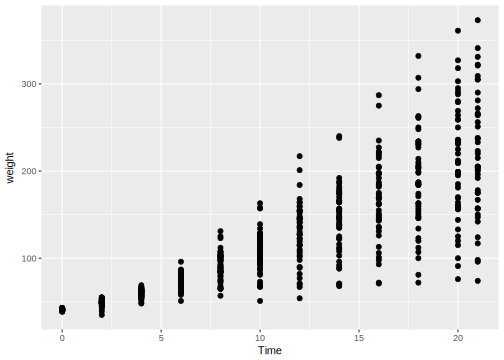
\includegraphics{Rprogramming_files/figure-latex/unnamed-chunk-30-1.png}

\begin{Shaded}
\begin{Highlighting}[]
\KeywordTok{qplot}\NormalTok{(acs}\OperatorTok{$}\NormalTok{BMI, acs}\OperatorTok{$}\NormalTok{LDLC)}
\NormalTok{## Warning: Removed 106 rows containing missing values}
\NormalTok{## (geom_point).}
\end{Highlighting}
\end{Shaded}

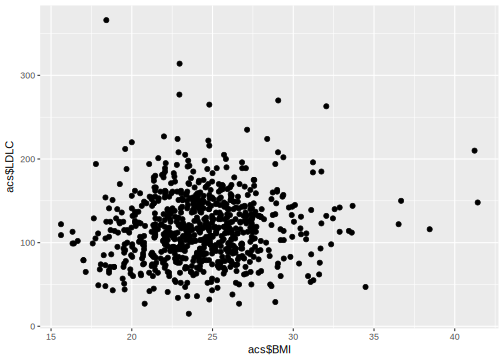
\includegraphics{Rprogramming_files/figure-latex/unnamed-chunk-31-1.png}

\begin{Shaded}
\begin{Highlighting}[]
\KeywordTok{ggplot}\NormalTok{(acs, }\KeywordTok{aes}\NormalTok{(}\DataTypeTok{x =}\NormalTok{ BMI, }\DataTypeTok{y =}\NormalTok{ LDLC)) }\OperatorTok{+}\StringTok{ }\KeywordTok{geom_point}\NormalTok{()}
\NormalTok{## Warning: Removed 106 rows containing missing values}
\NormalTok{## (geom_point).}
\end{Highlighting}
\end{Shaded}

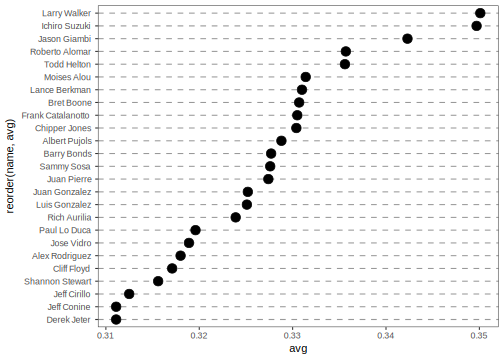
\includegraphics{Rprogramming_files/figure-latex/unnamed-chunk-31-2.png}

\section{Part1}\label{part1}

\begin{Shaded}
\begin{Highlighting}[]
\NormalTok{tophit <-}\StringTok{ }\NormalTok{tophitters2001[}\DecValTok{1}\OperatorTok{:}\DecValTok{25}\NormalTok{,]}
\NormalTok{tophit <-}\StringTok{ }\NormalTok{tophit[,}\KeywordTok{c}\NormalTok{(}\StringTok{"name"}\NormalTok{, }\StringTok{"lg"}\NormalTok{, }\StringTok{"avg"}\NormalTok{)]}

\CommentTok{# y축 이산형 그래프 }
\KeywordTok{ggplot}\NormalTok{(tophit, }\KeywordTok{aes}\NormalTok{(}\DataTypeTok{x =}\NormalTok{ avg, }\DataTypeTok{y =}\NormalTok{ name, }\DataTypeTok{col=}\NormalTok{lg)) }\OperatorTok{+}\StringTok{ }\KeywordTok{geom_point}\NormalTok{()}
\end{Highlighting}
\end{Shaded}

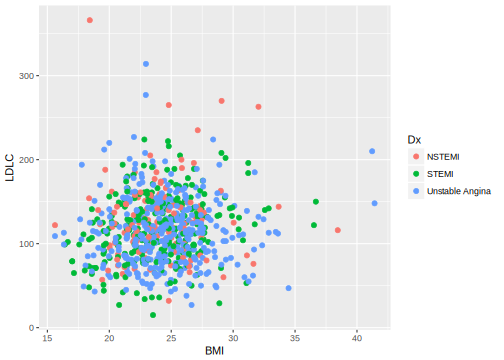
\includegraphics{Rprogramming_files/figure-latex/Part1-1.png}

\begin{Shaded}
\begin{Highlighting}[]

\KeywordTok{ggplot}\NormalTok{(acs, }\KeywordTok{aes}\NormalTok{(}\DataTypeTok{x =}\NormalTok{ BMI, }\DataTypeTok{y =}\NormalTok{ LDLC, }\DataTypeTok{col=}\NormalTok{Dx)) }\OperatorTok{+}\StringTok{ }\KeywordTok{geom_point}\NormalTok{()}
\NormalTok{## Warning: Removed 106 rows containing missing values}
\NormalTok{## (geom_point).}
\end{Highlighting}
\end{Shaded}

\includegraphics{Rprogramming_files/figure-latex/Part1-2.png}

\begin{Shaded}
\begin{Highlighting}[]


\CommentTok{# 그래프 정렬하기 & 그래프 격자 없애기 & 수평선 점선으로 바꾸기}
\KeywordTok{ggplot}\NormalTok{(tophit, }\KeywordTok{aes}\NormalTok{(}\DataTypeTok{x =}\NormalTok{ avg, }\DataTypeTok{y =} \KeywordTok{reorder}\NormalTok{(name, avg))) }\OperatorTok{+}\StringTok{ }\KeywordTok{geom_point}\NormalTok{(}\DataTypeTok{size =} \DecValTok{3}\NormalTok{) }\OperatorTok{+}\StringTok{ }\KeywordTok{theme_bw}\NormalTok{() }\OperatorTok{+}\StringTok{ }
\StringTok{  }\KeywordTok{theme}\NormalTok{(}\DataTypeTok{panel.grid.major.x =} \KeywordTok{element_blank}\NormalTok{(),}
        \DataTypeTok{panel.grid.minor.x =} \KeywordTok{element_blank}\NormalTok{(),}
        \DataTypeTok{panel.grid.major.y =} \KeywordTok{element_line}\NormalTok{(}\DataTypeTok{color =} \StringTok{"grey60"}\NormalTok{, }\DataTypeTok{linetype =} \StringTok{"dashed"}\NormalTok{))}
\end{Highlighting}
\end{Shaded}

\includegraphics{Rprogramming_files/figure-latex/Part1-3.png}

\begin{Shaded}
\begin{Highlighting}[]
\CommentTok{# x, y축 바꿔서 그치기 & 그래프 격자 없애기 & 수직선 점선으로 바꾸기 & X축 값 정의 및 회전}
\KeywordTok{ggplot}\NormalTok{(tophit, }\KeywordTok{aes}\NormalTok{(}\DataTypeTok{x =} \KeywordTok{reorder}\NormalTok{(name, avg), }\DataTypeTok{y =}\NormalTok{ avg)) }\OperatorTok{+}\StringTok{ }\KeywordTok{geom_point}\NormalTok{(}\DataTypeTok{size =} \DecValTok{3}\NormalTok{) }\OperatorTok{+}\StringTok{ }\KeywordTok{theme_bw}\NormalTok{() }\OperatorTok{+}\StringTok{ }
\StringTok{  }\KeywordTok{theme}\NormalTok{(}\DataTypeTok{axis.text.x =} \KeywordTok{element_text}\NormalTok{(}\DataTypeTok{angle =} \DecValTok{60}\NormalTok{, }\DataTypeTok{hjust =} \DecValTok{1}\NormalTok{),}
        \DataTypeTok{panel.grid.major.y =} \KeywordTok{element_blank}\NormalTok{(),}
        \DataTypeTok{panel.grid.minor.y =} \KeywordTok{element_blank}\NormalTok{(),}
        \DataTypeTok{panel.grid.major.x =} \KeywordTok{element_line}\NormalTok{(}\DataTypeTok{color =} \StringTok{"grey60"}\NormalTok{, }\DataTypeTok{linetype =} \StringTok{"dashed"}\NormalTok{))}
\end{Highlighting}
\end{Shaded}

\includegraphics{Rprogramming_files/figure-latex/unnamed-chunk-32-1.png}

\begin{Shaded}
\begin{Highlighting}[]


\CommentTok{# 두개 변수로 정의하여 그리기}
\NormalTok{nameorder <-}\StringTok{ }\NormalTok{tophit}\OperatorTok{$}\NormalTok{name[}\KeywordTok{order}\NormalTok{(tophit}\OperatorTok{$}\NormalTok{lg, tophit}\OperatorTok{$}\NormalTok{avg)]}
\NormalTok{tophit}\OperatorTok{$}\NormalTok{name <-}\StringTok{ }\KeywordTok{factor}\NormalTok{(tophit}\OperatorTok{$}\NormalTok{name, }\DataTypeTok{levels =}\NormalTok{ nameorder)}

\CommentTok{# 격자 선이 그래프의 끝에서 끝까지 횡단하지 않고, 점까지만 가도록 표현 [ geom_segment ]}
\KeywordTok{ggplot}\NormalTok{(tophit, }\KeywordTok{aes}\NormalTok{(}\DataTypeTok{x =}\NormalTok{ avg, }\DataTypeTok{y =}\NormalTok{ name)) }\OperatorTok{+}\StringTok{ }
\StringTok{  }\KeywordTok{geom_segment}\NormalTok{(}\KeywordTok{aes}\NormalTok{(}\DataTypeTok{yend =}\NormalTok{ name), }\DataTypeTok{xend =} \DecValTok{0}\NormalTok{, }\DataTypeTok{color =} \StringTok{"grey50"}\NormalTok{) }\OperatorTok{+}\StringTok{ }\KeywordTok{geom_point}\NormalTok{(}\DataTypeTok{size =} \DecValTok{3}\NormalTok{, }\KeywordTok{aes}\NormalTok{(}\DataTypeTok{color =}\NormalTok{ lg)) }\OperatorTok{+}\StringTok{ }
\StringTok{  }\KeywordTok{scale_color_brewer}\NormalTok{(}\DataTypeTok{palette =} \StringTok{"Set1"}\NormalTok{, }\DataTypeTok{limits =} \KeywordTok{c}\NormalTok{(}\StringTok{"NL"}\NormalTok{, }\StringTok{"AL"}\NormalTok{)) }\OperatorTok{+}\StringTok{ }\KeywordTok{theme_bw}\NormalTok{() }\OperatorTok{+}\StringTok{ }
\StringTok{  }\KeywordTok{theme}\NormalTok{(}\DataTypeTok{panel.grid.major.y =} \KeywordTok{element_blank}\NormalTok{(), }\DataTypeTok{legend.position =} \KeywordTok{c}\NormalTok{(}\DecValTok{1}\NormalTok{, }\FloatTok{0.55}\NormalTok{), }\CommentTok{# 범례를 그래프 안쪽으로 옮김 }
        \DataTypeTok{legend.justification =} \KeywordTok{c}\NormalTok{(}\DecValTok{1}\NormalTok{, }\FloatTok{0.5}\NormalTok{))}
\end{Highlighting}
\end{Shaded}

\includegraphics{Rprogramming_files/figure-latex/unnamed-chunk-32-2.png}

\begin{Shaded}
\begin{Highlighting}[]


\CommentTok{# 그룹 별 그래프 분할 }
\KeywordTok{ggplot}\NormalTok{(tophit, }\KeywordTok{aes}\NormalTok{(}\DataTypeTok{x =}\NormalTok{ avg, }\DataTypeTok{y =}\NormalTok{ name)) }\OperatorTok{+}\StringTok{ }
\StringTok{  }\KeywordTok{geom_segment}\NormalTok{(}\KeywordTok{aes}\NormalTok{(}\DataTypeTok{yend =}\NormalTok{ name), }\DataTypeTok{xend =} \DecValTok{0}\NormalTok{, }\DataTypeTok{color =} \StringTok{"grey50"}\NormalTok{) }\OperatorTok{+}\StringTok{ }\KeywordTok{geom_point}\NormalTok{(}\DataTypeTok{size =} \DecValTok{5}\NormalTok{, }\KeywordTok{aes}\NormalTok{(}\DataTypeTok{color =}\NormalTok{ lg)) }\OperatorTok{+}\StringTok{ }
\StringTok{  }\KeywordTok{scale_color_brewer}\NormalTok{(}\DataTypeTok{palette =} \StringTok{"Set1"}\NormalTok{, }\DataTypeTok{limits =} \KeywordTok{c}\NormalTok{(}\StringTok{"NL"}\NormalTok{, }\StringTok{"AL"}\NormalTok{), }\DataTypeTok{guide =} \OtherTok{FALSE}\NormalTok{) }\OperatorTok{+}\StringTok{ }\KeywordTok{theme_bw}\NormalTok{() }\OperatorTok{+}\StringTok{ }
\StringTok{  }\KeywordTok{theme}\NormalTok{(}\DataTypeTok{panel.grid.major.y =} \KeywordTok{element_blank}\NormalTok{()) }\OperatorTok{+}\StringTok{ }\KeywordTok{facet_grid}\NormalTok{(lg }\OperatorTok{~}\StringTok{ }\NormalTok{., }\DataTypeTok{scales =} \StringTok{"free_y"}\NormalTok{, }\DataTypeTok{space =} \StringTok{"free_y"}\NormalTok{) }
\end{Highlighting}
\end{Shaded}

\includegraphics{Rprogramming_files/figure-latex/unnamed-chunk-32-3.png}

\begin{Shaded}
\begin{Highlighting}[]


\CommentTok{# 그룹 별 데이터 구별}
\CommentTok{# 색상기준}
\KeywordTok{ggplot}\NormalTok{(heightweight, }\KeywordTok{aes}\NormalTok{(}\DataTypeTok{x =}\NormalTok{ ageYear, }\DataTypeTok{y =}\NormalTok{ heightIn, }\DataTypeTok{color =}\NormalTok{ sex)) }\OperatorTok{+}\StringTok{ }\KeywordTok{geom_point}\NormalTok{()}
\end{Highlighting}
\end{Shaded}

\includegraphics{Rprogramming_files/figure-latex/unnamed-chunk-32-4.png}

\begin{Shaded}
\begin{Highlighting}[]


\CommentTok{# 점 모양 기준}
\KeywordTok{ggplot}\NormalTok{(heightweight, }\KeywordTok{aes}\NormalTok{(}\DataTypeTok{x =}\NormalTok{ ageYear, }\DataTypeTok{y =}\NormalTok{ heightIn, }\DataTypeTok{shape =}\NormalTok{ sex)) }\OperatorTok{+}\StringTok{ }\KeywordTok{geom_point}\NormalTok{()}
\end{Highlighting}
\end{Shaded}

\includegraphics{Rprogramming_files/figure-latex/unnamed-chunk-32-5.png}

\begin{Shaded}
\begin{Highlighting}[]


\KeywordTok{ggplot}\NormalTok{(heightweight, }\KeywordTok{aes}\NormalTok{(}\DataTypeTok{x =}\NormalTok{ ageYear, }\DataTypeTok{y =}\NormalTok{ heightIn, }\DataTypeTok{color =}\NormalTok{ sex, }\DataTypeTok{shape =}\NormalTok{ sex)) }\OperatorTok{+}\StringTok{ }\KeywordTok{geom_point}\NormalTok{() }\OperatorTok{+}
\StringTok{  }\KeywordTok{scale_shape_manual}\NormalTok{(}\DataTypeTok{values =} \KeywordTok{c}\NormalTok{(}\DecValTok{1}\NormalTok{,}\DecValTok{2}\NormalTok{)) }\OperatorTok{+}\StringTok{ }\KeywordTok{scale_color_brewer}\NormalTok{(}\DataTypeTok{palette =} \StringTok{"Set1"}\NormalTok{)}
\end{Highlighting}
\end{Shaded}

\includegraphics{Rprogramming_files/figure-latex/unnamed-chunk-32-6.png}

\begin{Shaded}
\begin{Highlighting}[]


\KeywordTok{ggplot}\NormalTok{(heightweight, }\KeywordTok{aes}\NormalTok{(}\DataTypeTok{x =}\NormalTok{ ageYear, }\DataTypeTok{y =}\NormalTok{ heightIn, }\DataTypeTok{color =}\NormalTok{ sex, }\DataTypeTok{shape =}\NormalTok{ sex)) }\OperatorTok{+}\StringTok{ }\KeywordTok{geom_point}\NormalTok{() }\OperatorTok{+}
\StringTok{  }\KeywordTok{scale_shape_manual}\NormalTok{(}\DataTypeTok{values =} \KeywordTok{c}\NormalTok{(}\DecValTok{3}\NormalTok{,}\DecValTok{2}\NormalTok{)) }\OperatorTok{+}\StringTok{ }\KeywordTok{scale_color_brewer}\NormalTok{(}\DataTypeTok{palette =} \StringTok{"Set1"}\NormalTok{)}
\end{Highlighting}
\end{Shaded}

\includegraphics{Rprogramming_files/figure-latex/unnamed-chunk-32-7.png}

\begin{Shaded}
\begin{Highlighting}[]


\CommentTok{# 기준 정의에 따라 구별}
\NormalTok{hw <-heightweight}
\NormalTok{hw}\OperatorTok{$}\NormalTok{weightGroup <-}\StringTok{ }\KeywordTok{cut}\NormalTok{(hw}\OperatorTok{$}\NormalTok{weightLb, }\DataTypeTok{breaks =} \KeywordTok{c}\NormalTok{(}\OperatorTok{-}\OtherTok{Inf}\NormalTok{, }\DecValTok{100}\NormalTok{, }\OtherTok{Inf}\NormalTok{), }\DataTypeTok{labels =} \KeywordTok{c}\NormalTok{(}\StringTok{"< 100"}\NormalTok{, }\StringTok{">= 100"}\NormalTok{))}

\CommentTok{# x축이 이산형일 때 점들을 랜덤하게 조금식 이동시켜 표현 }
\KeywordTok{ggplot}\NormalTok{(ChickWeight, }\KeywordTok{aes}\NormalTok{(}\DataTypeTok{x =}\NormalTok{ Time, }\DataTypeTok{y =}\NormalTok{ weight)) }\OperatorTok{+}\StringTok{ }\KeywordTok{geom_point}\NormalTok{()}
\end{Highlighting}
\end{Shaded}

\includegraphics{Rprogramming_files/figure-latex/unnamed-chunk-32-8.png}

\begin{Shaded}
\begin{Highlighting}[]


\KeywordTok{ggplot}\NormalTok{(ChickWeight, }\KeywordTok{aes}\NormalTok{(}\DataTypeTok{x =}\NormalTok{ Time, }\DataTypeTok{y =}\NormalTok{ weight)) }\OperatorTok{+}\StringTok{ }\KeywordTok{geom_jitter}\NormalTok{() }\CommentTok{# 이동 적용}
\end{Highlighting}
\end{Shaded}

\includegraphics{Rprogramming_files/figure-latex/unnamed-chunk-32-9.png}

\begin{Shaded}
\begin{Highlighting}[]


\CommentTok{# 적합된 회귀선 추가하기}
\NormalTok{sp <-}\StringTok{ }\KeywordTok{ggplot}\NormalTok{(ChickWeight, }\KeywordTok{aes}\NormalTok{(}\DataTypeTok{x =}\NormalTok{ Time, }\DataTypeTok{y =}\NormalTok{ weight)) }
\NormalTok{sp }\OperatorTok{+}\StringTok{ }\KeywordTok{geom_point}\NormalTok{(}\DataTypeTok{color =} \StringTok{"blue"}\NormalTok{) }\OperatorTok{+}\StringTok{ }\KeywordTok{stat_smooth}\NormalTok{(}\DataTypeTok{method =}\NormalTok{ lm, }\DataTypeTok{se =} \OtherTok{TRUE}\NormalTok{, }\DataTypeTok{color =} \StringTok{"red"}\NormalTok{) }
\end{Highlighting}
\end{Shaded}

\includegraphics{Rprogramming_files/figure-latex/unnamed-chunk-32-10.png}

\begin{Shaded}
\begin{Highlighting}[]


\NormalTok{sp }\OperatorTok{+}\StringTok{ }\KeywordTok{geom_jitter}\NormalTok{(}\DataTypeTok{color =} \StringTok{"blue"}\NormalTok{) }\OperatorTok{+}\StringTok{ }\KeywordTok{stat_smooth}\NormalTok{(}\DataTypeTok{method =}\NormalTok{ lm, }\DataTypeTok{se =} \OtherTok{TRUE}\NormalTok{, }\DataTypeTok{color =} \StringTok{"red"}\NormalTok{)}
\end{Highlighting}
\end{Shaded}

\includegraphics{Rprogramming_files/figure-latex/unnamed-chunk-32-11.png}

\begin{Shaded}
\begin{Highlighting}[]


\CommentTok{#그룹 별 회귀선 추가하기}
\NormalTok{sps <-}\StringTok{ }\KeywordTok{ggplot}\NormalTok{(heightweight, }\KeywordTok{aes}\NormalTok{(}\DataTypeTok{x =}\NormalTok{ ageYear, }\DataTypeTok{y =}\NormalTok{ heightIn, }\DataTypeTok{color =}\NormalTok{ sex)) }\OperatorTok{+}\StringTok{ }
\StringTok{  }\KeywordTok{geom_point}\NormalTok{() }\OperatorTok{+}\StringTok{ }\KeywordTok{scale_color_brewer}\NormalTok{(}\DataTypeTok{palette =} \StringTok{"Set1"}\NormalTok{)}
\NormalTok{sps }\OperatorTok{+}\StringTok{ }\KeywordTok{geom_smooth}\NormalTok{()}
\NormalTok{## `geom_smooth()` using method = 'loess'}
\end{Highlighting}
\end{Shaded}

\includegraphics{Rprogramming_files/figure-latex/unnamed-chunk-32-12.png}

\begin{Shaded}
\begin{Highlighting}[]


\CommentTok{# 예측값 실제값 그래프로 표현하기 (함수)}
\NormalTok{predictvals <-}\StringTok{ }\ControlFlowTok{function}\NormalTok{(model, xvar, yvar, }\DataTypeTok{xrange =} \OtherTok{NULL}\NormalTok{, }\DataTypeTok{sample =} \DecValTok{100}\NormalTok{, ...)\{}
  \ControlFlowTok{if}\NormalTok{(}\KeywordTok{is.null}\NormalTok{(xrange))\{}
    \ControlFlowTok{if}\NormalTok{(}\KeywordTok{any}\NormalTok{(}\KeywordTok{class}\NormalTok{(model) }\OperatorTok\StringTok{ }\KeywordTok{c}\NormalTok{(}\StringTok{"lm"}\NormalTok{, }\StringTok{"glm"}\NormalTok{)))}
\NormalTok{      xrange <-}\StringTok{ }\KeywordTok{range}\NormalTok{(model}\OperatorTok{$}\NormalTok{model[[xvar]])}
    \ControlFlowTok{else} \ControlFlowTok{if}\NormalTok{(}\KeywordTok{any}\NormalTok{(}\KeywordTok{class}\NormalTok{(model) }\OperatorTok\StringTok{ "loess"}\NormalTok{))}
\NormalTok{      xrange <-}\StringTok{ }\KeywordTok{range}\NormalTok{(model}\OperatorTok{$}\NormalTok{x)}
\NormalTok{  \}}
  
\NormalTok{  newdata <-}\StringTok{ }\KeywordTok{data.frame}\NormalTok{(}\DataTypeTok{x =} \KeywordTok{seq}\NormalTok{(xrange[}\DecValTok{1}\NormalTok{], xrange[}\DecValTok{2}\NormalTok{], }\DataTypeTok{length.out =}\NormalTok{ sample))}
  \KeywordTok{names}\NormalTok{(newdata) <-}\StringTok{ }\NormalTok{xvar}
\NormalTok{  newdata[[yvar]] <-}\StringTok{ }\KeywordTok{predict}\NormalTok{(model, }\DataTypeTok{newdata =}\NormalTok{ newdata, ...)}
\NormalTok{  newdata}
\NormalTok{\}}

\NormalTok{modlinear <-}\StringTok{ }\KeywordTok{lm}\NormalTok{(heightIn }\OperatorTok{~}\StringTok{ }\NormalTok{ageYear, heightweight)}
\NormalTok{modloess <-}\StringTok{ }\KeywordTok{loess}\NormalTok{(heightIn }\OperatorTok{~}\StringTok{ }\NormalTok{ageYear, heightweight)}

\NormalTok{lm_predicted   <-}\StringTok{ }\KeywordTok{predictvals}\NormalTok{(modlinear, }\StringTok{"ageYear"}\NormalTok{, }\StringTok{"heightIn"}\NormalTok{)}
\NormalTok{loess_predicted <-}\StringTok{ }\KeywordTok{predictvals}\NormalTok{(modloess, }\StringTok{"ageYear"}\NormalTok{, }\StringTok{"heightIn"}\NormalTok{)}

\NormalTok{sp <-}\StringTok{ }\KeywordTok{ggplot}\NormalTok{(heightweight, }\KeywordTok{aes}\NormalTok{(}\DataTypeTok{x =}\NormalTok{ ageYear, }\DataTypeTok{y =}\NormalTok{ heightIn)) }\OperatorTok{+}
\StringTok{  }\KeywordTok{geom_point}\NormalTok{(}\DataTypeTok{color =} \StringTok{"grey40"}\NormalTok{)}
\NormalTok{sp }\OperatorTok{+}\StringTok{ }\KeywordTok{geom_line}\NormalTok{(}\DataTypeTok{data =}\NormalTok{ lm_predicted, }\DataTypeTok{color =} \StringTok{"red"}\NormalTok{, }\DataTypeTok{size =} \FloatTok{0.8}\NormalTok{) }\OperatorTok{+}
\StringTok{  }\KeywordTok{geom_line}\NormalTok{(}\DataTypeTok{data =}\NormalTok{ loess_predicted, }\DataTypeTok{color =} \StringTok{"blue"}\NormalTok{, }\DataTypeTok{size =} \FloatTok{0.8}\NormalTok{)}
\end{Highlighting}
\end{Shaded}

\includegraphics{Rprogramming_files/figure-latex/unnamed-chunk-32-13.png}

\begin{Shaded}
\begin{Highlighting}[]


\CommentTok{#산점도의 점에 라벨 붙이기}
\NormalTok{sp <-}\StringTok{ }\KeywordTok{ggplot}\NormalTok{(}\KeywordTok{subset}\NormalTok{(countries, Year }\OperatorTok{==}\StringTok{ }\DecValTok{2009} \OperatorTok{&}\StringTok{ }\NormalTok{healthexp }\OperatorTok{>}\StringTok{ }\DecValTok{2000}\NormalTok{),}
             \KeywordTok{aes}\NormalTok{(}\DataTypeTok{x =}\NormalTok{ healthexp, }\DataTypeTok{y =}\NormalTok{ infmortality)) }\OperatorTok{+}\StringTok{ }\KeywordTok{geom_point}\NormalTok{()}

\CommentTok{# 특정 값에 특정 단어로 라벨 붙이기}
\NormalTok{sp }\OperatorTok{+}\StringTok{ }\KeywordTok{annotate}\NormalTok{(}\StringTok{"text"}\NormalTok{, }\DataTypeTok{x =} \DecValTok{4350}\NormalTok{, }\DataTypeTok{y =} \FloatTok{5.4}\NormalTok{, }\DataTypeTok{label =} \StringTok{"Canada"}\NormalTok{) }\OperatorTok{+}\StringTok{ }
\StringTok{  }\KeywordTok{annotate}\NormalTok{(}\StringTok{"text"}\NormalTok{, }\DataTypeTok{x =} \DecValTok{7400}\NormalTok{, }\DataTypeTok{y =} \FloatTok{6.8}\NormalTok{, }\DataTypeTok{label =} \StringTok{"USA"}\NormalTok{)}
\end{Highlighting}
\end{Shaded}

\includegraphics{Rprogramming_files/figure-latex/unnamed-chunk-32-14.png}

\begin{Shaded}
\begin{Highlighting}[]


\CommentTok{# 데이터 값을 라벨로 붙이기}
\NormalTok{sp }\OperatorTok{+}\StringTok{ }\KeywordTok{geom_text}\NormalTok{(}\KeywordTok{aes}\NormalTok{(}\DataTypeTok{label =}\NormalTok{ Name), }\DataTypeTok{size =} \DecValTok{4}\NormalTok{)}
\end{Highlighting}
\end{Shaded}

\includegraphics{Rprogramming_files/figure-latex/unnamed-chunk-32-15.png}

\begin{Shaded}
\begin{Highlighting}[]


\CommentTok{# 라벨의 위치를 데이터값보다 조금 크게 설정}
\NormalTok{sp }\OperatorTok{+}\StringTok{ }\KeywordTok{geom_text}\NormalTok{(}\KeywordTok{aes}\NormalTok{(}\DataTypeTok{y =}\NormalTok{ infmortality }\OperatorTok{+}\StringTok{ }\FloatTok{0.1}\NormalTok{, }\DataTypeTok{label =}\NormalTok{ Name), }\DataTypeTok{size =} \DecValTok{4}\NormalTok{, }\DataTypeTok{vjust =} \DecValTok{0}\NormalTok{)}
\end{Highlighting}
\end{Shaded}

\includegraphics{Rprogramming_files/figure-latex/unnamed-chunk-32-16.png}

\begin{Shaded}
\begin{Highlighting}[]


\NormalTok{sp }\OperatorTok{+}\StringTok{ }\KeywordTok{geom_text}\NormalTok{(}\KeywordTok{aes}\NormalTok{(}\DataTypeTok{x =}\NormalTok{ healthexp }\OperatorTok{+}\StringTok{ }\DecValTok{100}\NormalTok{, }\DataTypeTok{label =}\NormalTok{ Name), }\DataTypeTok{size =} \DecValTok{4}\NormalTok{, }\DataTypeTok{hjust =} \DecValTok{0}\NormalTok{)}
\end{Highlighting}
\end{Shaded}

\includegraphics{Rprogramming_files/figure-latex/unnamed-chunk-32-17.png}

\begin{Shaded}
\begin{Highlighting}[]


\CommentTok{# 특정 값만 라벨 붙이기}
\NormalTok{cdat <-}\StringTok{ }\KeywordTok{subset}\NormalTok{(countries, Year }\OperatorTok{==}\StringTok{ }\DecValTok{2009} \OperatorTok{&}\StringTok{ }\NormalTok{healthexp }\OperatorTok{>}\StringTok{ }\DecValTok{2000}\NormalTok{)}
\NormalTok{cdat}\OperatorTok{$}\NormalTok{Name1 <-}\StringTok{ }\NormalTok{cdat}\OperatorTok{$}\NormalTok{Name }
\NormalTok{idx <-}\StringTok{ }\NormalTok{cdat}\OperatorTok{$}\NormalTok{Name }\OperatorTok\StringTok{ }\KeywordTok{c}\NormalTok{(}\StringTok{"Andorra"}\NormalTok{, }\StringTok{"France"}\NormalTok{, }\StringTok{"Canada"}\NormalTok{) }
\NormalTok{cdat}\OperatorTok{$}\NormalTok{Name1[}\OperatorTok{!}\NormalTok{idx] <-}\StringTok{ }\OtherTok{NA}
\KeywordTok{ggplot}\NormalTok{(cdat, }\KeywordTok{aes}\NormalTok{(}\DataTypeTok{x =}\NormalTok{ healthexp, }\DataTypeTok{y =}\NormalTok{ infmortality)) }\OperatorTok{+}\StringTok{ }\KeywordTok{geom_point}\NormalTok{() }\OperatorTok{+}\StringTok{ }\KeywordTok{geom_text}\NormalTok{(}\KeywordTok{aes}\NormalTok{(}\DataTypeTok{y =}\NormalTok{ infmortality }\OperatorTok{+}\StringTok{ }\FloatTok{0.1}\NormalTok{, }\DataTypeTok{label =}\NormalTok{ Name1), }\DataTypeTok{size =} \DecValTok{4}\NormalTok{, }\DataTypeTok{vjust =} \DecValTok{0}\NormalTok{)}
\NormalTok{## Warning: Removed 24 rows containing missing values}
\NormalTok{## (geom_text).}
\end{Highlighting}
\end{Shaded}

\includegraphics{Rprogramming_files/figure-latex/unnamed-chunk-32-18.png}

\begin{Shaded}
\begin{Highlighting}[]
\NormalTok{## Warning: Removed 24 rows containing missing values (geom_text).}
\end{Highlighting}
\end{Shaded}

\section{Part2}\label{part2}

\begin{Shaded}
\begin{Highlighting}[]

\CommentTok{# 거품그래프(balloon plot)}
\NormalTok{hec <-}\StringTok{ }\NormalTok{HairEyeColor[,,}\StringTok{"Male"}\NormalTok{] }\OperatorTok{+}\StringTok{ }\NormalTok{HairEyeColor[,,}\StringTok{"Female"}\NormalTok{]}
\NormalTok{hec <-}\StringTok{ }\KeywordTok{melt}\NormalTok{(hec, }\DataTypeTok{value.name =} \StringTok{"count"}\NormalTok{) }
\KeywordTok{ggplot}\NormalTok{(hec, }\KeywordTok{aes}\NormalTok{(}\DataTypeTok{x =}\NormalTok{ Eye, }\DataTypeTok{y =}\NormalTok{ Hair)) }\OperatorTok{+}\StringTok{ }\KeywordTok{geom_point}\NormalTok{(}\KeywordTok{aes}\NormalTok{(}\DataTypeTok{size =}\NormalTok{ count), }\DataTypeTok{shape =} \DecValTok{21}\NormalTok{, }\DataTypeTok{color =} \StringTok{"black"}\NormalTok{, }\DataTypeTok{fill =} \StringTok{"cornsilk"}\NormalTok{) }\OperatorTok{+}\StringTok{ }
\StringTok{  }\KeywordTok{scale_size_area}\NormalTok{(}\DataTypeTok{max_size =} \DecValTok{20}\NormalTok{, }\DataTypeTok{guide =} \OtherTok{FALSE}\NormalTok{) }\OperatorTok{+}\StringTok{ }
\StringTok{  }\KeywordTok{geom_text}\NormalTok{(}\KeywordTok{aes}\NormalTok{(}\DataTypeTok{y =} \KeywordTok{as.numeric}\NormalTok{(Hair)}\OperatorTok{-}\KeywordTok{sqrt}\NormalTok{(count)}\OperatorTok{/}\DecValTok{22}\NormalTok{, }\DataTypeTok{label =}\NormalTok{ count), }\DataTypeTok{vjust =} \DecValTok{1}\NormalTok{, }\DataTypeTok{color =} \StringTok{"grey60"}\NormalTok{, }\DataTypeTok{size =} \DecValTok{4}\NormalTok{)}
\end{Highlighting}
\end{Shaded}

\includegraphics{Rprogramming_files/figure-latex/part2-1.png}

\begin{Shaded}
\begin{Highlighting}[]


\CommentTok{# 산점도 행렬 만들기}
\NormalTok{c2009 <-}\StringTok{ }\KeywordTok{subset}\NormalTok{(countries, Year }\OperatorTok{==}\StringTok{ }\DecValTok{2009}\NormalTok{, }\DataTypeTok{select =} \KeywordTok{c}\NormalTok{(Name, GDP, laborrate, healthexp, infmortality)) }
\KeywordTok{plot}\NormalTok{(c2009[,}\DecValTok{2}\OperatorTok{:}\DecValTok{5}\NormalTok{])}
\end{Highlighting}
\end{Shaded}

\includegraphics{Rprogramming_files/figure-latex/part2-2.png}

\begin{Shaded}
\begin{Highlighting}[]


\NormalTok{panel.hist <-}\StringTok{ }\ControlFlowTok{function}\NormalTok{(x, ...)}
\NormalTok{\{}
\NormalTok{  usr <-}\StringTok{ }\KeywordTok{par}\NormalTok{(}\StringTok{"usr"}\NormalTok{); }\KeywordTok{on.exit}\NormalTok{(}\KeywordTok{par}\NormalTok{(usr))}
  \KeywordTok{par}\NormalTok{(}\DataTypeTok{usr =} \KeywordTok{c}\NormalTok{(usr[}\DecValTok{1}\OperatorTok{:}\DecValTok{2}\NormalTok{], }\DecValTok{0}\NormalTok{, }\FloatTok{1.5}\NormalTok{) )}
\NormalTok{  h <-}\StringTok{ }\KeywordTok{hist}\NormalTok{(x, }\DataTypeTok{plot =} \OtherTok{FALSE}\NormalTok{)}
\NormalTok{  breaks <-}\StringTok{ }\NormalTok{h}\OperatorTok{$}\NormalTok{breaks; nB <-}\StringTok{ }\KeywordTok{length}\NormalTok{(breaks)}
\NormalTok{  y <-}\StringTok{ }\NormalTok{h}\OperatorTok{$}\NormalTok{counts; y <-}\StringTok{ }\NormalTok{y}\OperatorTok{/}\KeywordTok{max}\NormalTok{(y)}
  \KeywordTok{rect}\NormalTok{(breaks[}\OperatorTok{-}\NormalTok{nB], }\DecValTok{0}\NormalTok{, breaks[}\OperatorTok{-}\DecValTok{1}\NormalTok{], y, }\DataTypeTok{col =} \StringTok{"cyan"}\NormalTok{, ...)}
\NormalTok{\}}
\NormalTok{panel.cor <-}\StringTok{ }\ControlFlowTok{function}\NormalTok{(x, y, }\DataTypeTok{digits =} \DecValTok{2}\NormalTok{, }\DataTypeTok{prefix =} \StringTok{""}\NormalTok{, cex.cor, ...)}
\NormalTok{\{}
\NormalTok{  usr <-}\StringTok{ }\KeywordTok{par}\NormalTok{(}\StringTok{"usr"}\NormalTok{); }\KeywordTok{on.exit}\NormalTok{(}\KeywordTok{par}\NormalTok{(usr))}
  \KeywordTok{par}\NormalTok{(}\DataTypeTok{usr =} \KeywordTok{c}\NormalTok{(}\DecValTok{0}\NormalTok{, }\DecValTok{1}\NormalTok{, }\DecValTok{0}\NormalTok{, }\DecValTok{1}\NormalTok{))}
\NormalTok{  r <-}\StringTok{ }\KeywordTok{abs}\NormalTok{(}\KeywordTok{cor}\NormalTok{(x, y))}
\NormalTok{  txt <-}\StringTok{ }\KeywordTok{format}\NormalTok{(}\KeywordTok{c}\NormalTok{(r, }\FloatTok{0.123456789}\NormalTok{), }\DataTypeTok{digits =}\NormalTok{ digits)[}\DecValTok{1}\NormalTok{]}
\NormalTok{  txt <-}\StringTok{ }\KeywordTok{paste0}\NormalTok{(prefix, txt)}
  \ControlFlowTok{if}\NormalTok{(}\KeywordTok{missing}\NormalTok{(cex.cor)) cex.cor <-}\StringTok{ }\FloatTok{0.8}\OperatorTok{/}\KeywordTok{strwidth}\NormalTok{(txt)}
  \KeywordTok{text}\NormalTok{(}\FloatTok{0.5}\NormalTok{, }\FloatTok{0.5}\NormalTok{, txt, }\DataTypeTok{cex =}\NormalTok{ cex.cor }\OperatorTok{*}\StringTok{ }\NormalTok{r)}
\NormalTok{\}}
\NormalTok{panel.lm <-}\StringTok{ }\ControlFlowTok{function}\NormalTok{(x, y, }\DataTypeTok{col =} \KeywordTok{par}\NormalTok{(}\StringTok{"col"}\NormalTok{), }\DataTypeTok{bg =} \OtherTok{NA}\NormalTok{, }\DataTypeTok{pch =} \KeywordTok{par}\NormalTok{(}\StringTok{"pch"}\NormalTok{), }\DataTypeTok{cex =} \DecValTok{1}\NormalTok{, }\DataTypeTok{col.smooth =} \StringTok{"black"}\NormalTok{, ...)\{}
  \KeywordTok{points}\NormalTok{(x, y, }\DataTypeTok{pch =}\NormalTok{ pch, }\DataTypeTok{col =}\NormalTok{ col, }\DataTypeTok{bg =}\NormalTok{ bg, }\DataTypeTok{cex =}\NormalTok{ cex)}
  \KeywordTok{abline}\NormalTok{(stats}\OperatorTok{::}\KeywordTok{lm}\NormalTok{(y }\OperatorTok{~}\StringTok{ }\NormalTok{x), }\DataTypeTok{col =}\NormalTok{ col.smooth, ...)}
\NormalTok{\}}
\CommentTok{# 데이터에 대한 LOWESS선(평활선) 추가 }
\KeywordTok{pairs}\NormalTok{(c2009[,}\DecValTok{2}\OperatorTok{:}\DecValTok{5}\NormalTok{], }\DataTypeTok{pch =} \StringTok{"."}\NormalTok{, }\DataTypeTok{upper.panel =}\NormalTok{ panel.cor, }\DataTypeTok{diag.panel =}\NormalTok{ panel.hist, }\DataTypeTok{lower.panel =}\NormalTok{ panel.lm)}
\end{Highlighting}
\end{Shaded}

\includegraphics{Rprogramming_files/figure-latex/part2-3.png}

\begin{Shaded}
\begin{Highlighting}[]


\CommentTok{# 데이터에 대한 회귀적합선 추가 }
\KeywordTok{pairs}\NormalTok{(c2009[,}\DecValTok{2}\OperatorTok{:}\DecValTok{5}\NormalTok{], }\DataTypeTok{pch =} \StringTok{"."}\NormalTok{, }\DataTypeTok{upper.panel =}\NormalTok{ panel.cor, }\DataTypeTok{diag.panel =}\NormalTok{ panel.hist, }\DataTypeTok{lower.panel =}\NormalTok{ panel.smooth)}
\end{Highlighting}
\end{Shaded}

\includegraphics{Rprogramming_files/figure-latex/part2-4.png}

\begin{Shaded}
\begin{Highlighting}[]


\NormalTok{######################################################################################}
\NormalTok{## scatter + line plot  (geom_point/ geom_line)}
\NormalTok{######################################################################################}
\KeywordTok{plot}\NormalTok{(pressure}\OperatorTok{$}\NormalTok{temperature, pressure}\OperatorTok{$}\NormalTok{pressure, }\DataTypeTok{type =} \StringTok{"l"}\NormalTok{)}
\KeywordTok{points}\NormalTok{(pressure}\OperatorTok{$}\NormalTok{temperature, pressure}\OperatorTok{$}\NormalTok{pressure)}
\end{Highlighting}
\end{Shaded}

\includegraphics{Rprogramming_files/figure-latex/part2-5.png}

\begin{Shaded}
\begin{Highlighting}[]


\KeywordTok{qplot}\NormalTok{(temperature, pressure, }\DataTypeTok{data =}\NormalTok{ pressure, }\DataTypeTok{geom =} \KeywordTok{c}\NormalTok{(}\StringTok{"line"}\NormalTok{, }\StringTok{"point"}\NormalTok{))}
\end{Highlighting}
\end{Shaded}

\includegraphics{Rprogramming_files/figure-latex/part2-6.png}

\begin{Shaded}
\begin{Highlighting}[]


\KeywordTok{ggplot}\NormalTok{(pressure, }\KeywordTok{aes}\NormalTok{(}\DataTypeTok{x =}\NormalTok{ temperature, }\DataTypeTok{y =}\NormalTok{ pressure)) }\OperatorTok{+}\StringTok{ }\KeywordTok{geom_point}\NormalTok{() }\OperatorTok{+}\StringTok{ }\KeywordTok{geom_line}\NormalTok{()}
\end{Highlighting}
\end{Shaded}

\includegraphics{Rprogramming_files/figure-latex/part2-7.png}

\begin{Shaded}
\begin{Highlighting}[]


\NormalTok{######################################################################################}
\NormalTok{## line plot  (geom_line)}
\NormalTok{######################################################################################}
\KeywordTok{ggplot}\NormalTok{(BOD, }\KeywordTok{aes}\NormalTok{(}\DataTypeTok{x =}\NormalTok{ Time, }\DataTypeTok{y =}\NormalTok{ demand)) }\OperatorTok{+}\StringTok{ }\KeywordTok{geom_line}\NormalTok{() }\OperatorTok{+}\StringTok{ }\KeywordTok{ylim}\NormalTok{(}\DecValTok{0}\NormalTok{, }\KeywordTok{max}\NormalTok{(BOD}\OperatorTok{$}\NormalTok{demand))}
\end{Highlighting}
\end{Shaded}

\includegraphics{Rprogramming_files/figure-latex/part2-8.png}

\begin{Shaded}
\begin{Highlighting}[]


\KeywordTok{ggplot}\NormalTok{(BOD, }\KeywordTok{aes}\NormalTok{(}\DataTypeTok{x =}\NormalTok{ Time, }\DataTypeTok{y =}\NormalTok{ demand)) }\OperatorTok{+}\StringTok{ }\KeywordTok{geom_line}\NormalTok{() }\OperatorTok{+}\StringTok{ }\KeywordTok{expand_limits}\NormalTok{(}\DataTypeTok{y =} \DecValTok{0}\NormalTok{)}
\end{Highlighting}
\end{Shaded}

\includegraphics{Rprogramming_files/figure-latex/part2-9.png}

\begin{Shaded}
\begin{Highlighting}[]


\KeywordTok{ggplot}\NormalTok{(BOD, }\KeywordTok{aes}\NormalTok{(}\DataTypeTok{x =}\NormalTok{ Time, }\DataTypeTok{y =}\NormalTok{ demand)) }\OperatorTok{+}\StringTok{ }\KeywordTok{geom_line}\NormalTok{() }\OperatorTok{+}\StringTok{ }\KeywordTok{geom_point}\NormalTok{()}
\end{Highlighting}
\end{Shaded}

\includegraphics{Rprogramming_files/figure-latex/part2-10.png}

\begin{Shaded}
\begin{Highlighting}[]


\CommentTok{# 이산형 변수값에 따른 구분 }
\NormalTok{tg <-}\StringTok{ }\KeywordTok{ddply}\NormalTok{(ToothGrowth, }\KeywordTok{c}\NormalTok{(}\StringTok{"supp"}\NormalTok{, }\StringTok{"dose"}\NormalTok{), summarize, }\DataTypeTok{length =} \KeywordTok{mean}\NormalTok{(len))}
\CommentTok{# 색상으로 구분}
\KeywordTok{ggplot}\NormalTok{(tg, }\KeywordTok{aes}\NormalTok{(}\DataTypeTok{x =}\NormalTok{ dose, }\DataTypeTok{y =}\NormalTok{ length, }\DataTypeTok{color =}\NormalTok{ supp)) }\OperatorTok{+}\StringTok{ }\KeywordTok{geom_line}\NormalTok{()}
\end{Highlighting}
\end{Shaded}

\includegraphics{Rprogramming_files/figure-latex/part2-11.png}

\begin{Shaded}
\begin{Highlighting}[]


\KeywordTok{ggplot}\NormalTok{(tg, }\KeywordTok{aes}\NormalTok{(}\DataTypeTok{x =} \KeywordTok{factor}\NormalTok{(dose), }\DataTypeTok{y =}\NormalTok{ length, }\DataTypeTok{color =}\NormalTok{ supp, }\DataTypeTok{group =}\NormalTok{ supp)) }\OperatorTok{+}\StringTok{ }\KeywordTok{geom_line}\NormalTok{()}
\end{Highlighting}
\end{Shaded}

\includegraphics{Rprogramming_files/figure-latex/part2-12.png}

\begin{Shaded}
\begin{Highlighting}[]


\CommentTok{# group = supp 주의! : 이 명령문이 없으면 데이터를 어떻게 묶어서 그릴지 모름}
\CommentTok{# Line type으로 구분}
\KeywordTok{ggplot}\NormalTok{(tg, }\KeywordTok{aes}\NormalTok{(}\DataTypeTok{x =}\NormalTok{ dose, }\DataTypeTok{y =}\NormalTok{ length, }\DataTypeTok{linetype =}\NormalTok{ supp)) }\OperatorTok{+}\StringTok{ }\KeywordTok{geom_line}\NormalTok{()}
\end{Highlighting}
\end{Shaded}

\includegraphics{Rprogramming_files/figure-latex/part2-13.png}

\begin{Shaded}
\begin{Highlighting}[]


\CommentTok{# 점 형태로 구분}
\KeywordTok{ggplot}\NormalTok{(tg, }\KeywordTok{aes}\NormalTok{(}\DataTypeTok{x =}\NormalTok{ dose, }\DataTypeTok{y =}\NormalTok{ length, }\DataTypeTok{shape =}\NormalTok{ supp)) }\OperatorTok{+}\StringTok{ }\KeywordTok{geom_line}\NormalTok{() }\OperatorTok{+}\StringTok{ }\KeywordTok{geom_point}\NormalTok{(}\DataTypeTok{size =} \DecValTok{4}\NormalTok{)}
\end{Highlighting}
\end{Shaded}

\includegraphics{Rprogramming_files/figure-latex/part2-14.png}

\begin{Shaded}
\begin{Highlighting}[]


\CommentTok{# 점 색상으로 구분}
\KeywordTok{ggplot}\NormalTok{(tg, }\KeywordTok{aes}\NormalTok{(}\DataTypeTok{x =}\NormalTok{ dose, }\DataTypeTok{y =}\NormalTok{ length, }\DataTypeTok{fill =}\NormalTok{ supp)) }\OperatorTok{+}\StringTok{ }\KeywordTok{geom_line}\NormalTok{() }\OperatorTok{+}\StringTok{ }\KeywordTok{geom_point}\NormalTok{(}\DataTypeTok{size =} \DecValTok{4}\NormalTok{, }\DataTypeTok{shape =} \DecValTok{21}\NormalTok{)}
\end{Highlighting}
\end{Shaded}

\includegraphics{Rprogramming_files/figure-latex/part2-15.png}

\begin{Shaded}
\begin{Highlighting}[]


\CommentTok{# 두 선이 겹칠때 하나의 선을 옆으로 이동시켜 표현  }
\KeywordTok{ggplot}\NormalTok{(tg, }\KeywordTok{aes}\NormalTok{(}\DataTypeTok{x =}\NormalTok{ dose, }\DataTypeTok{y =}\NormalTok{ length, }\DataTypeTok{shape =}\NormalTok{ supp)) }\OperatorTok{+}\StringTok{ }\KeywordTok{geom_line}\NormalTok{(}\DataTypeTok{position =} \KeywordTok{position_dodge}\NormalTok{(}\FloatTok{0.1}\NormalTok{)) }\OperatorTok{+}\StringTok{ }
\StringTok{  }\KeywordTok{geom_point}\NormalTok{(}\DataTypeTok{position =} \KeywordTok{position_dodge}\NormalTok{(}\FloatTok{0.1}\NormalTok{), }\DataTypeTok{size =} \DecValTok{4}\NormalTok{)}
\end{Highlighting}
\end{Shaded}

\includegraphics{Rprogramming_files/figure-latex/part2-16.png}

\begin{Shaded}
\begin{Highlighting}[]


\CommentTok{# 선 형태 바꾸기 [ linetype ]}
\KeywordTok{ggplot}\NormalTok{(tg, }\KeywordTok{aes}\NormalTok{(}\DataTypeTok{x =}\NormalTok{ dose, }\DataTypeTok{y =}\NormalTok{ length, }\DataTypeTok{color =}\NormalTok{ supp)) }\OperatorTok{+}\StringTok{ }\KeywordTok{geom_line}\NormalTok{(}\DataTypeTok{linetype =} \StringTok{"dashed"}\NormalTok{) }\OperatorTok{+}
\StringTok{  }\KeywordTok{geom_point}\NormalTok{(}\DataTypeTok{shape =} \DecValTok{22}\NormalTok{, }\DataTypeTok{size =} \DecValTok{3}\NormalTok{, }\DataTypeTok{fill =} \StringTok{"white"}\NormalTok{)}
\end{Highlighting}
\end{Shaded}

\includegraphics{Rprogramming_files/figure-latex/part2-17.png}

\section{Part3}\label{part3}

\begin{Shaded}
\begin{Highlighting}[]

\CommentTok{# 점 형태 바꾸기 [ shape ]}
\NormalTok{#################################}
\NormalTok{pd <-}\StringTok{ }\KeywordTok{position_dodge}\NormalTok{(}\FloatTok{0.2}\NormalTok{)       }\CommentTok{#}
\NormalTok{#################################}

\KeywordTok{ggplot}\NormalTok{(tg, }\KeywordTok{aes}\NormalTok{(}\DataTypeTok{x =}\NormalTok{ dose, }\DataTypeTok{y =}\NormalTok{ length, }\DataTypeTok{fill =}\NormalTok{ supp)) }\OperatorTok{+}\StringTok{ }\KeywordTok{geom_line}\NormalTok{(}\DataTypeTok{position =}\NormalTok{ pd) }\OperatorTok{+}\StringTok{ }
\StringTok{  }\KeywordTok{geom_point}\NormalTok{(}\DataTypeTok{shape =} \DecValTok{21}\NormalTok{, }\DataTypeTok{size =} \DecValTok{5}\NormalTok{, }\DataTypeTok{position =}\NormalTok{ pd) }\OperatorTok{+}\StringTok{ }
\StringTok{  }\KeywordTok{scale_fill_manual}\NormalTok{(}\DataTypeTok{values =} \KeywordTok{c}\NormalTok{(}\StringTok{"black"}\NormalTok{, }\StringTok{"white"}\NormalTok{))}
\end{Highlighting}
\end{Shaded}

\includegraphics{Rprogramming_files/figure-latex/part3-1.png}

\begin{Shaded}
\begin{Highlighting}[]


\CommentTok{# sample Data}
\NormalTok{sunspotyear <-}\StringTok{ }\KeywordTok{data.frame}\NormalTok{(}\DataTypeTok{Year     =} \KeywordTok{as.numeric}\NormalTok{(}\KeywordTok{time}\NormalTok{(sunspot.year)),}
                          \DataTypeTok{Sunspots =} \KeywordTok{as.numeric}\NormalTok{(sunspot.year))}
\CommentTok{# 음영 영역 그래프 그리기}
\KeywordTok{ggplot}\NormalTok{(sunspotyear, }\KeywordTok{aes}\NormalTok{(}\DataTypeTok{x =}\NormalTok{ Year, }\DataTypeTok{y =}\NormalTok{ Sunspots)) }\OperatorTok{+}\StringTok{ }\KeywordTok{geom_area}\NormalTok{()}
\end{Highlighting}
\end{Shaded}

\includegraphics{Rprogramming_files/figure-latex/part3-2.png}

\begin{Shaded}
\begin{Highlighting}[]


\CommentTok{# 음영 투명도 설정하기 [ alpha ]}
\KeywordTok{ggplot}\NormalTok{(sunspotyear, }\KeywordTok{aes}\NormalTok{(}\DataTypeTok{x =}\NormalTok{ Year, }\DataTypeTok{y =}\NormalTok{ Sunspots)) }\OperatorTok{+}\StringTok{ }\KeywordTok{geom_area}\NormalTok{(}\DataTypeTok{color =} \StringTok{"black"}\NormalTok{, }\DataTypeTok{fill =} \StringTok{"blue"}\NormalTok{, }\DataTypeTok{alpha =} \FloatTok{0.5}\NormalTok{)}
\end{Highlighting}
\end{Shaded}

\includegraphics{Rprogramming_files/figure-latex/part3-3.png}

\begin{Shaded}
\begin{Highlighting}[]


\CommentTok{# 누적 영역 그래프 그리기}
\KeywordTok{ggplot}\NormalTok{(uspopage, }\KeywordTok{aes}\NormalTok{(}\DataTypeTok{x =}\NormalTok{ Year, }\DataTypeTok{y =}\NormalTok{ Thousands, }\DataTypeTok{fill =}\NormalTok{ AgeGroup)) }\OperatorTok{+}\StringTok{ }\KeywordTok{geom_area}\NormalTok{()}
\end{Highlighting}
\end{Shaded}

\includegraphics{Rprogramming_files/figure-latex/part3-4.png}

\begin{Shaded}
\begin{Highlighting}[]


\CommentTok{# 영역색상 그라데이션 넣기}
\KeywordTok{ggplot}\NormalTok{(uspopage, }\KeywordTok{aes}\NormalTok{(}\DataTypeTok{x =}\NormalTok{ Year, }\DataTypeTok{y =}\NormalTok{ Thousands, }\DataTypeTok{fill =}\NormalTok{ AgeGroup)) }\OperatorTok{+}\StringTok{ }\KeywordTok{geom_area}\NormalTok{(}\DataTypeTok{color =} \StringTok{"black"}\NormalTok{, }\DataTypeTok{size =} \FloatTok{0.2}\NormalTok{, }\DataTypeTok{alpha =} \FloatTok{0.4}\NormalTok{) }\OperatorTok{+}\StringTok{ }
\StringTok{  }\KeywordTok{scale_fill_brewer}\NormalTok{(}\DataTypeTok{palette =} \StringTok{"Blues"}\NormalTok{, }\DataTypeTok{breaks =} \KeywordTok{rev}\NormalTok{(}\KeywordTok{levels}\NormalTok{(uspopage}\OperatorTok{$}\NormalTok{AgeGroup)))}
\end{Highlighting}
\end{Shaded}

\includegraphics{Rprogramming_files/figure-latex/part3-5.png}

\begin{Shaded}
\begin{Highlighting}[]


\CommentTok{# 데이터 순서정렬하기 & 양쪽 테두리 지우기 }
\KeywordTok{ggplot}\NormalTok{(uspopage, }\KeywordTok{aes}\NormalTok{(}\DataTypeTok{x =}\NormalTok{ Year, }\DataTypeTok{y =}\NormalTok{ Thousands, }\DataTypeTok{fill =}\NormalTok{ AgeGroup, }\DataTypeTok{order =} \KeywordTok{desc}\NormalTok{(AgeGroup))) }\OperatorTok{+}\StringTok{ }
\StringTok{  }\KeywordTok{geom_area}\NormalTok{(}\DataTypeTok{color =} \OtherTok{NA}\NormalTok{, }\DataTypeTok{alpha =} \FloatTok{0.4}\NormalTok{) }\OperatorTok{+}\StringTok{ }\KeywordTok{scale_fill_brewer}\NormalTok{(}\DataTypeTok{palette =} \StringTok{"Blues"}\NormalTok{) }\OperatorTok{+}\StringTok{ }\KeywordTok{geom_line}\NormalTok{(}\DataTypeTok{position =} \StringTok{"stack"}\NormalTok{, }\DataTypeTok{size =} \FloatTok{0.2}\NormalTok{)}
\end{Highlighting}
\end{Shaded}

\includegraphics{Rprogramming_files/figure-latex/part3-6.png}

\begin{Shaded}
\begin{Highlighting}[]


\CommentTok{#  비율 누적 영역 그래프 그리기}
\NormalTok{uspopage_prop <-}\StringTok{ }\KeywordTok{ddply}\NormalTok{(uspopage, }\StringTok{"Year"}\NormalTok{, transform, }\DataTypeTok{Percent =}\NormalTok{ Thousands }\OperatorTok{/}\StringTok{ }\KeywordTok{sum}\NormalTok{(Thousands) }\OperatorTok{*}\StringTok{ }\DecValTok{100}\NormalTok{) }
\KeywordTok{ggplot}\NormalTok{(uspopage_prop, }\KeywordTok{aes}\NormalTok{(}\DataTypeTok{x =}\NormalTok{ Year, }\DataTypeTok{y =}\NormalTok{ Percent, }\DataTypeTok{fill =}\NormalTok{ AgeGroup)) }\OperatorTok{+}\StringTok{ }\KeywordTok{geom_area}\NormalTok{(}\DataTypeTok{color =} \StringTok{"black"}\NormalTok{, }\DataTypeTok{size =} \FloatTok{0.2}\NormalTok{, }\DataTypeTok{alpha =} \FloatTok{0.4}\NormalTok{) }\OperatorTok{+}\StringTok{ }
\StringTok{  }\KeywordTok{scale_fill_brewer}\NormalTok{(}\DataTypeTok{palette =} \StringTok{"Blues"}\NormalTok{, }\DataTypeTok{breaks =} \KeywordTok{rev}\NormalTok{(}\KeywordTok{levels}\NormalTok{(uspopage}\OperatorTok{$}\NormalTok{AgeGroup)))}
\end{Highlighting}
\end{Shaded}

\includegraphics{Rprogramming_files/figure-latex/part3-7.png}

\begin{Shaded}
\begin{Highlighting}[]


\CommentTok{# 그래프에 신뢰 영역 추가하기}
\NormalTok{clim <-}\StringTok{ }\KeywordTok{subset}\NormalTok{(climate, Source }\OperatorTok{==}\StringTok{ "Berkeley"}\NormalTok{, }\DataTypeTok{select =} \KeywordTok{c}\NormalTok{(}\StringTok{"Year"}\NormalTok{, }\StringTok{"Anomaly10y"}\NormalTok{, }\StringTok{"Unc10y"}\NormalTok{))}
\CommentTok{# 신뢰영역 음영으로 표현 }
\KeywordTok{ggplot}\NormalTok{(clim, }\KeywordTok{aes}\NormalTok{(}\DataTypeTok{x =}\NormalTok{ Year, }\DataTypeTok{y =}\NormalTok{ Anomaly10y)) }\OperatorTok{+}\StringTok{ }
\StringTok{  }\KeywordTok{geom_ribbon}\NormalTok{(}\KeywordTok{aes}\NormalTok{(}\DataTypeTok{ymin =}\NormalTok{ Anomaly10y }\OperatorTok{-}\StringTok{ }\NormalTok{Unc10y, }\DataTypeTok{ymax =}\NormalTok{ Anomaly10y }\OperatorTok{+}\StringTok{ }\NormalTok{Unc10y), }\DataTypeTok{alpha =} \FloatTok{0.2}\NormalTok{) }\OperatorTok{+}
\StringTok{  }\KeywordTok{geom_line}\NormalTok{()}
\end{Highlighting}
\end{Shaded}

\includegraphics{Rprogramming_files/figure-latex/part3-8.png}

\begin{Shaded}
\begin{Highlighting}[]


\CommentTok{# 신뢰영역 점선으로 표현}
\KeywordTok{ggplot}\NormalTok{(clim, }\KeywordTok{aes}\NormalTok{(}\DataTypeTok{x =}\NormalTok{ Year, }\DataTypeTok{y =}\NormalTok{ Anomaly10y)) }\OperatorTok{+}\StringTok{ }
\StringTok{  }\KeywordTok{geom_line}\NormalTok{(}\KeywordTok{aes}\NormalTok{(}\DataTypeTok{y =}\NormalTok{ Anomaly10y }\OperatorTok{-}\StringTok{ }\NormalTok{Unc10y), }\DataTypeTok{linetype =} \StringTok{"dotted"}\NormalTok{) }\OperatorTok{+}
\StringTok{  }\KeywordTok{geom_line}\NormalTok{(}\KeywordTok{aes}\NormalTok{(}\DataTypeTok{y =}\NormalTok{ Anomaly10y }\OperatorTok{+}\StringTok{ }\NormalTok{Unc10y), }\DataTypeTok{linetype =} \StringTok{"dotted"}\NormalTok{) }\OperatorTok{+}
\StringTok{  }\KeywordTok{geom_line}\NormalTok{()}
\end{Highlighting}
\end{Shaded}

\includegraphics{Rprogramming_files/figure-latex/part3-9.png}

\begin{Shaded}
\begin{Highlighting}[]


\CommentTok{# }
\NormalTok{######################################################################################}
\NormalTok{## barplot  (geom_bar)}
\NormalTok{######################################################################################}
\KeywordTok{barplot}\NormalTok{(BOD}\OperatorTok{$}\NormalTok{demand, }\DataTypeTok{names.arg =}\NormalTok{ BOD}\OperatorTok{$}\NormalTok{Time)}
\end{Highlighting}
\end{Shaded}

\includegraphics{Rprogramming_files/figure-latex/part3-10.png}

\begin{Shaded}
\begin{Highlighting}[]


\KeywordTok{barplot}\NormalTok{(}\KeywordTok{table}\NormalTok{(mtcars}\OperatorTok{$}\NormalTok{cyl))}
\end{Highlighting}
\end{Shaded}

\includegraphics{Rprogramming_files/figure-latex/part3-11.png}

\begin{Shaded}
\begin{Highlighting}[]


\CommentTok{# x값을 숫자로 인식}
\CommentTok{# qplot(BOD$Time, BOD$demand, geom = "bar", stat = "identity")}
\KeywordTok{ggplot}\NormalTok{(BOD, }\KeywordTok{aes}\NormalTok{(}\DataTypeTok{x =}\NormalTok{ Time, }\DataTypeTok{y =}\NormalTok{ demand)) }\OperatorTok{+}\StringTok{ }\KeywordTok{geom_bar}\NormalTok{(}\DataTypeTok{stat =} \StringTok{"identity"}\NormalTok{)}
\end{Highlighting}
\end{Shaded}

\includegraphics{Rprogramming_files/figure-latex/part3-12.png}

\begin{Shaded}
\begin{Highlighting}[]


\CommentTok{# x값을 요인으로 변환}
\CommentTok{# qplot(as.factor(BOD$Time), BOD$demand, geom = "bar", stat = "identity")}
\KeywordTok{ggplot}\NormalTok{(BOD, }\KeywordTok{aes}\NormalTok{(}\DataTypeTok{x =} \KeywordTok{factor}\NormalTok{(Time), }\DataTypeTok{y =}\NormalTok{ demand)) }\OperatorTok{+}\StringTok{ }\KeywordTok{geom_bar}\NormalTok{(}\DataTypeTok{stat =} \StringTok{"identity"}\NormalTok{)}
\end{Highlighting}
\end{Shaded}

\includegraphics{Rprogramming_files/figure-latex/part3-13.png}

\begin{Shaded}
\begin{Highlighting}[]


\CommentTok{# 막대 색상 채우기/테두리 설정하기 (fill : 채우기/ colour(or color) : 테두리)}
\KeywordTok{ggplot}\NormalTok{(pg_mean, }\KeywordTok{aes}\NormalTok{(}\DataTypeTok{x =}\NormalTok{ group, }\DataTypeTok{y =}\NormalTok{ weight)) }\OperatorTok{+}\StringTok{ }\KeywordTok{geom_bar}\NormalTok{(}\DataTypeTok{stat =} \StringTok{"identity"}\NormalTok{, }\DataTypeTok{fill =} \StringTok{"lightblue"}\NormalTok{, }\DataTypeTok{colour =} \StringTok{"black"}\NormalTok{)}
\end{Highlighting}
\end{Shaded}

\includegraphics{Rprogramming_files/figure-latex/part3-14.png}

\begin{Shaded}
\begin{Highlighting}[]


\CommentTok{# 막대 묶어서 표현하기(나누어 표현하고 싶은 변수를 색상으로 지정)  }
\KeywordTok{ggplot}\NormalTok{(cabbage_exp, }\KeywordTok{aes}\NormalTok{(}\DataTypeTok{x =}\NormalTok{ Date, }\DataTypeTok{y =}\NormalTok{ Weight, }\DataTypeTok{fill =}\NormalTok{ Cultivar)) }\OperatorTok{+}\StringTok{ }\KeywordTok{geom_bar}\NormalTok{(}\DataTypeTok{stat =} \StringTok{"identity"}\NormalTok{, }\DataTypeTok{position =} \StringTok{"dodge"}\NormalTok{)}
\end{Highlighting}
\end{Shaded}

\includegraphics{Rprogramming_files/figure-latex/part3-15.png}

\begin{Shaded}
\begin{Highlighting}[]


\CommentTok{# dodge : "피하다"라는 의미로 막대를 새로운 값을 기준으로 나누어 표현 }
\KeywordTok{ggplot}\NormalTok{(cabbage_exp, }\KeywordTok{aes}\NormalTok{(}\DataTypeTok{x =}\NormalTok{ Date, }\DataTypeTok{y =}\NormalTok{ Weight, }\DataTypeTok{fill =}\NormalTok{ Cultivar)) }\OperatorTok{+}\StringTok{ }\KeywordTok{geom_bar}\NormalTok{(}\DataTypeTok{stat =} \StringTok{"identity"}\NormalTok{, }\DataTypeTok{position =} \StringTok{"dodge"}\NormalTok{, }\DataTypeTok{color =} \StringTok{"black"}\NormalTok{) }\OperatorTok{+}\StringTok{ }
\StringTok{  }\KeywordTok{scale_fill_brewer}\NormalTok{(}\DataTypeTok{palette =} \StringTok{"Pastel1"}\NormalTok{)}
\end{Highlighting}
\end{Shaded}

\includegraphics{Rprogramming_files/figure-latex/part3-16.png}

\section{Part4}\label{part4}

\begin{Shaded}
\begin{Highlighting}[]

\CommentTok{# 빈도수 막대 그래프 그리기 }
\CommentTok{# x가 이산형}
\KeywordTok{ggplot}\NormalTok{(diamonds, }\KeywordTok{aes}\NormalTok{(}\DataTypeTok{x =}\NormalTok{ cut)) }\OperatorTok{+}\StringTok{ }\KeywordTok{geom_bar}\NormalTok{()}
\end{Highlighting}
\end{Shaded}

\includegraphics{Rprogramming_files/figure-latex/part4-1.png}

\begin{Shaded}
\begin{Highlighting}[]


\CommentTok{# x가 연속형}
\KeywordTok{ggplot}\NormalTok{(diamonds, }\KeywordTok{aes}\NormalTok{(}\DataTypeTok{x =}\NormalTok{ carat)) }\OperatorTok{+}\StringTok{ }\KeywordTok{geom_bar}\NormalTok{()}
\end{Highlighting}
\end{Shaded}

\includegraphics{Rprogramming_files/figure-latex/part4-2.png}

\begin{Shaded}
\begin{Highlighting}[]


\CommentTok{# 막대 색상 넣기/ 축 이름 정의하기(reorder) }
\NormalTok{upc <-}\StringTok{ }\KeywordTok{subset}\NormalTok{(uspopchange, }\KeywordTok{rank}\NormalTok{(Change) }\OperatorTok{>}\StringTok{ }\DecValTok{40}\NormalTok{)}
\KeywordTok{ggplot}\NormalTok{(upc, }\KeywordTok{aes}\NormalTok{(}\DataTypeTok{x =} \KeywordTok{reorder}\NormalTok{(Abb, Change), }\DataTypeTok{y =}\NormalTok{ Change, }\DataTypeTok{fill =}\NormalTok{ Region)) }\OperatorTok{+}\StringTok{ }\KeywordTok{geom_bar}\NormalTok{(}\DataTypeTok{stat =} \StringTok{"identity"}\NormalTok{, }\DataTypeTok{color =} \StringTok{"black"}\NormalTok{) }\OperatorTok{+}
\StringTok{  }\KeywordTok{scale_fill_manual}\NormalTok{(}\DataTypeTok{values =} \KeywordTok{c}\NormalTok{(}\StringTok{"#669933"}\NormalTok{, }\StringTok{"#FFCC66"}\NormalTok{)) }\OperatorTok{+}\StringTok{ }\KeywordTok{xlab}\NormalTok{(}\StringTok{"State"}\NormalTok{)}
\end{Highlighting}
\end{Shaded}

\includegraphics{Rprogramming_files/figure-latex/part4-3.png}

\begin{Shaded}
\begin{Highlighting}[]


\CommentTok{# 양수/음수 다른 색상으로 표현 (구분 inde를 만들어 색상 변수로 지정)}
\NormalTok{csub <-}\StringTok{ }\KeywordTok{subset}\NormalTok{(climate, Source }\OperatorTok{==}\StringTok{ "Berkeley"} \OperatorTok{&}\StringTok{ }\NormalTok{Year }\OperatorTok{>=}\StringTok{ }\DecValTok{1900}\NormalTok{ )}
\NormalTok{csub}\OperatorTok{$}\NormalTok{pos <-}\StringTok{ }\NormalTok{csub}\OperatorTok{$}\NormalTok{Anomaly10y }\OperatorTok{>=}\StringTok{ }\DecValTok{0}
\KeywordTok{ggplot}\NormalTok{(csub, }\KeywordTok{aes}\NormalTok{(}\DataTypeTok{x =}\NormalTok{ Year, }\DataTypeTok{y =}\NormalTok{ Anomaly10y, }\DataTypeTok{fill =}\NormalTok{ pos)) }\OperatorTok{+}\StringTok{ }\KeywordTok{geom_bar}\NormalTok{(}\DataTypeTok{stat =} \StringTok{"identity"}\NormalTok{, }\DataTypeTok{position =} \StringTok{"identity"}\NormalTok{)}
\end{Highlighting}
\end{Shaded}

\includegraphics{Rprogramming_files/figure-latex/part4-4.png}

\begin{Shaded}
\begin{Highlighting}[]


\CommentTok{# 막대 그래프 테두리 두께 설정(size) / 범례 지우기(guide = FALSE)}
\KeywordTok{ggplot}\NormalTok{(csub, }\KeywordTok{aes}\NormalTok{(}\DataTypeTok{x =}\NormalTok{ Year, }\DataTypeTok{y =}\NormalTok{ Anomaly10y, }\DataTypeTok{fill =}\NormalTok{ pos)) }\OperatorTok{+}\StringTok{ }\KeywordTok{geom_bar}\NormalTok{(}\DataTypeTok{stat =} \StringTok{"identity"}\NormalTok{, }\DataTypeTok{position =} \StringTok{"identity"}\NormalTok{, }\DataTypeTok{color =} \StringTok{"black"}\NormalTok{, }\DataTypeTok{size =} \FloatTok{0.0001}\NormalTok{) }\OperatorTok{+}\StringTok{ }
\StringTok{  }\KeywordTok{scale_fill_manual}\NormalTok{(}\DataTypeTok{values =} \KeywordTok{c}\NormalTok{(}\StringTok{"#CCEEFF"}\NormalTok{, }\StringTok{"#FFDDDD"}\NormalTok{), }\DataTypeTok{guide =} \OtherTok{FALSE}\NormalTok{)}
\end{Highlighting}
\end{Shaded}

\includegraphics{Rprogramming_files/figure-latex/part4-5.png}

\begin{Shaded}
\begin{Highlighting}[]


\CommentTok{# 막대 너비/ 간격 조절하기(width : 최대 너비는 1)}
\KeywordTok{ggplot}\NormalTok{(pg_mean, }\KeywordTok{aes}\NormalTok{(}\DataTypeTok{x =}\NormalTok{ group, }\DataTypeTok{y =}\NormalTok{ weight)) }\OperatorTok{+}\StringTok{ }\KeywordTok{geom_bar}\NormalTok{(}\DataTypeTok{stat =} \StringTok{"identity"}\NormalTok{, }\DataTypeTok{width =} \FloatTok{0.5}\NormalTok{)}
\end{Highlighting}
\end{Shaded}

\includegraphics{Rprogramming_files/figure-latex/part4-6.png}

\begin{Shaded}
\begin{Highlighting}[]


\CommentTok{# 막대 그룹 간의 간격 조절하기 (default : 0.9) }
\KeywordTok{ggplot}\NormalTok{(cabbage_exp, }\KeywordTok{aes}\NormalTok{(}\DataTypeTok{x =}\NormalTok{ Date, }\DataTypeTok{y =}\NormalTok{ Weight, }\DataTypeTok{fill =}\NormalTok{ Cultivar)) }\OperatorTok{+}\StringTok{ }\KeywordTok{geom_bar}\NormalTok{(}\DataTypeTok{stat =} \StringTok{"identity"}\NormalTok{, }\DataTypeTok{width =} \FloatTok{0.4}\NormalTok{, }\DataTypeTok{position =} \StringTok{"dodge"}\NormalTok{)}
\end{Highlighting}
\end{Shaded}

\includegraphics{Rprogramming_files/figure-latex/part4-7.png}

\begin{Shaded}
\begin{Highlighting}[]


\CommentTok{# 막대 그룹 내부간의 간격 조절 (default : 0.9)}
\KeywordTok{ggplot}\NormalTok{(cabbage_exp, }\KeywordTok{aes}\NormalTok{(}\DataTypeTok{x =}\NormalTok{ Date, }\DataTypeTok{y =}\NormalTok{ Weight, }\DataTypeTok{fill =}\NormalTok{ Cultivar)) }\OperatorTok{+}\StringTok{ }\KeywordTok{geom_bar}\NormalTok{(}\DataTypeTok{stat =} \StringTok{"identity"}\NormalTok{, }\DataTypeTok{width =} \FloatTok{0.3}\NormalTok{, }\DataTypeTok{position =} \KeywordTok{position_dodge}\NormalTok{(}\FloatTok{0.5}\NormalTok{))}
\end{Highlighting}
\end{Shaded}

\includegraphics{Rprogramming_files/figure-latex/part4-8.png}

\begin{Shaded}
\begin{Highlighting}[]


\CommentTok{# 범례 순서 바꾸기 (reverse = TRUE) }
\KeywordTok{ggplot}\NormalTok{(cabbage_exp, }\KeywordTok{aes}\NormalTok{(}\DataTypeTok{x =}\NormalTok{ Date, }\DataTypeTok{y =}\NormalTok{ Weight, }\DataTypeTok{fill =}\NormalTok{ Cultivar)) }\OperatorTok{+}\StringTok{ }\KeywordTok{geom_bar}\NormalTok{(}\DataTypeTok{stat =} \StringTok{"identity"}\NormalTok{) }\OperatorTok{+}\StringTok{ }\KeywordTok{guides}\NormalTok{(}\DataTypeTok{fill =} \KeywordTok{guide_legend}\NormalTok{(}\DataTypeTok{reverse =} \OtherTok{TRUE}\NormalTok{))}
\end{Highlighting}
\end{Shaded}

\includegraphics{Rprogramming_files/figure-latex/part4-9.png}

\begin{Shaded}
\begin{Highlighting}[]


\CommentTok{# 막대 쌓는 순서 바꾸기  }
\KeywordTok{ggplot}\NormalTok{(cabbage_exp, }\KeywordTok{aes}\NormalTok{(}\DataTypeTok{x =}\NormalTok{ Date, }\DataTypeTok{y =}\NormalTok{ Weight, }\DataTypeTok{fill =}\NormalTok{ Cultivar, }\DataTypeTok{order =} \KeywordTok{desc}\NormalTok{(Cultivar))) }\OperatorTok{+}\StringTok{ }\KeywordTok{geom_bar}\NormalTok{(}\DataTypeTok{stat =} \StringTok{"identity"}\NormalTok{)}
\end{Highlighting}
\end{Shaded}

\includegraphics{Rprogramming_files/figure-latex/part4-10.png}

\begin{Shaded}
\begin{Highlighting}[]


\CommentTok{# 비율 누적 막대 그래프 그리기(막대 전체가 100%가 되도록)}
\NormalTok{ce <-}\StringTok{ }\KeywordTok{ddply}\NormalTok{(cabbage_exp, }\StringTok{"Date"}\NormalTok{, transform, }\DataTypeTok{percent_weight =}\NormalTok{ Weight }\OperatorTok{/}\StringTok{ }\KeywordTok{sum}\NormalTok{(Weight) }\OperatorTok{*}\StringTok{ }\DecValTok{100}\NormalTok{)}
\KeywordTok{ggplot}\NormalTok{(ce, }\KeywordTok{aes}\NormalTok{(}\DataTypeTok{x =}\NormalTok{ Date, }\DataTypeTok{y =}\NormalTok{ percent_weight, }\DataTypeTok{fill =}\NormalTok{ Cultivar)) }\OperatorTok{+}\StringTok{ }\KeywordTok{geom_bar}\NormalTok{(}\DataTypeTok{stat =} \StringTok{"identity"}\NormalTok{)}
\end{Highlighting}
\end{Shaded}

\includegraphics{Rprogramming_files/figure-latex/part4-11.png}

\begin{Shaded}
\begin{Highlighting}[]


\CommentTok{# 막대에 라벨 추가하기 [ geom_text ]}
\CommentTok{# 선 상단 [ vjust < 0 ]}
\KeywordTok{ggplot}\NormalTok{(cabbage_exp, }\KeywordTok{aes}\NormalTok{(}\DataTypeTok{x =} \KeywordTok{interaction}\NormalTok{(Date, Cultivar), }\DataTypeTok{y =}\NormalTok{ Weight)) }\OperatorTok{+}\StringTok{ }\KeywordTok{geom_bar}\NormalTok{(}\DataTypeTok{stat =} \StringTok{"identity"}\NormalTok{) }\OperatorTok{+}\StringTok{ }
\StringTok{  }\KeywordTok{geom_text}\NormalTok{(}\KeywordTok{aes}\NormalTok{(}\DataTypeTok{label =}\NormalTok{ Weight), }\DataTypeTok{vjust =} \OperatorTok{-}\FloatTok{0.2}\NormalTok{)}
\end{Highlighting}
\end{Shaded}

\includegraphics{Rprogramming_files/figure-latex/part4-12.png}

\begin{Shaded}
\begin{Highlighting}[]


\CommentTok{# 선 하단 [ vjust > 0 ]}
\KeywordTok{ggplot}\NormalTok{(cabbage_exp, }\KeywordTok{aes}\NormalTok{(}\DataTypeTok{x =} \KeywordTok{interaction}\NormalTok{(Date, Cultivar), }\DataTypeTok{y =}\NormalTok{ Weight)) }\OperatorTok{+}\StringTok{ }\KeywordTok{geom_bar}\NormalTok{(}\DataTypeTok{stat =} \StringTok{"identity"}\NormalTok{) }\OperatorTok{+}\StringTok{ }
\StringTok{  }\KeywordTok{geom_text}\NormalTok{(}\KeywordTok{aes}\NormalTok{(}\DataTypeTok{label =}\NormalTok{ Weight), }\DataTypeTok{vjust =} \FloatTok{1.5}\NormalTok{, }\DataTypeTok{color =} \StringTok{"white"}\NormalTok{)}
\end{Highlighting}
\end{Shaded}

\includegraphics{Rprogramming_files/figure-latex/part4-13.png}

\begin{Shaded}
\begin{Highlighting}[]


\CommentTok{# 그래프 범위 설정}
\CommentTok{# max(데이터)로 지정}
\KeywordTok{ggplot}\NormalTok{(cabbage_exp, }\KeywordTok{aes}\NormalTok{(}\DataTypeTok{x =} \KeywordTok{interaction}\NormalTok{(Date, Cultivar), }\DataTypeTok{y =}\NormalTok{ Weight)) }\OperatorTok{+}\StringTok{ }\KeywordTok{geom_bar}\NormalTok{(}\DataTypeTok{stat =} \StringTok{"identity"}\NormalTok{) }\OperatorTok{+}
\StringTok{  }\KeywordTok{geom_text}\NormalTok{(}\KeywordTok{aes}\NormalTok{(}\DataTypeTok{label =}\NormalTok{ Weight), }\DataTypeTok{vjust =} \OperatorTok{-}\FloatTok{0.2}\NormalTok{) }\OperatorTok{+}\StringTok{ }\KeywordTok{ylim}\NormalTok{(}\DecValTok{0}\NormalTok{, }\KeywordTok{max}\NormalTok{(cabbage_exp}\OperatorTok{$}\NormalTok{Weight) }\OperatorTok{*}\StringTok{ }\FloatTok{1.05}\NormalTok{)}
\end{Highlighting}
\end{Shaded}

\includegraphics{Rprogramming_files/figure-latex/part4-14.png}

\begin{Shaded}
\begin{Highlighting}[]


\CommentTok{# 막대의 상단보다 조금 높은 위치로 지정(데이터에 따라 자동 조정)}
\KeywordTok{ggplot}\NormalTok{(cabbage_exp, }\KeywordTok{aes}\NormalTok{(}\DataTypeTok{x =} \KeywordTok{interaction}\NormalTok{(Date, Cultivar), }\DataTypeTok{y =}\NormalTok{ Weight)) }\OperatorTok{+}\StringTok{ }\KeywordTok{geom_bar}\NormalTok{(}\DataTypeTok{stat =} \StringTok{"identity"}\NormalTok{) }\OperatorTok{+}
\StringTok{  }\KeywordTok{geom_text}\NormalTok{(}\KeywordTok{aes}\NormalTok{(}\DataTypeTok{y =}\NormalTok{ Weight }\OperatorTok{+}\StringTok{ }\FloatTok{0.1}\NormalTok{, }\DataTypeTok{label =}\NormalTok{ Weight)) }
\end{Highlighting}
\end{Shaded}

\includegraphics{Rprogramming_files/figure-latex/part4-15.png}

\begin{Shaded}
\begin{Highlighting}[]


\CommentTok{# 누적 합계 그래프 그리기}
\NormalTok{ce <-}\StringTok{ }\KeywordTok{arrange}\NormalTok{(cabbage_exp, Date, Cultivar)}
\NormalTok{ce <-}\StringTok{ }\KeywordTok{ddply}\NormalTok{(ce, }\StringTok{"Date"}\NormalTok{, transform, }\DataTypeTok{label =} \KeywordTok{cumsum}\NormalTok{(Weight))}
\CommentTok{# ddply(data.frame, 그룹 기준 마지막 변수)}
\KeywordTok{ggplot}\NormalTok{(ce, }\KeywordTok{aes}\NormalTok{(}\DataTypeTok{x =}\NormalTok{ Date, }\DataTypeTok{y =}\NormalTok{ Weight, }\DataTypeTok{fill =}\NormalTok{ Cultivar)) }\OperatorTok{+}\StringTok{ }\KeywordTok{geom_bar}\NormalTok{(}\DataTypeTok{stat =} \StringTok{"identity"}\NormalTok{, }\DataTypeTok{color =} \StringTok{"black"}\NormalTok{) }\OperatorTok{+}\StringTok{ }
\StringTok{  }\KeywordTok{geom_text}\NormalTok{(}\KeywordTok{aes}\NormalTok{(}\DataTypeTok{y =}\NormalTok{ label, }\DataTypeTok{label =} \KeywordTok{paste}\NormalTok{(}\KeywordTok{format}\NormalTok{(Weight, }\DataTypeTok{nsmall=}\DecValTok{2}\NormalTok{), }\StringTok{"kg"}\NormalTok{)), }\DataTypeTok{size =} \DecValTok{6}\NormalTok{, }\DataTypeTok{vjust =} \FloatTok{1.5}\NormalTok{) }\OperatorTok{+}\StringTok{ }
\StringTok{  }\KeywordTok{guides}\NormalTok{(}\DataTypeTok{fill =} \KeywordTok{guide_legend}\NormalTok{(}\DataTypeTok{reverse =} \OtherTok{TRUE}\NormalTok{)) }\OperatorTok{+}\StringTok{ }\KeywordTok{scale_fill_brewer}\NormalTok{(}\DataTypeTok{palette =} \StringTok{"Pastel1"}\NormalTok{)}
\end{Highlighting}
\end{Shaded}

\includegraphics{Rprogramming_files/figure-latex/part4-16.png}

\begin{Shaded}
\begin{Highlighting}[]


\NormalTok{######################################################################################}
\NormalTok{## histogram  (geom_histogram)}
\NormalTok{######################################################################################}
\KeywordTok{hist}\NormalTok{(mtcars}\OperatorTok{$}\NormalTok{mpg)}
\end{Highlighting}
\end{Shaded}

\includegraphics{Rprogramming_files/figure-latex/part4-17.png}

\begin{Shaded}
\begin{Highlighting}[]


\CommentTok{# 상자(bin) 개수 지정}
\KeywordTok{hist}\NormalTok{(mtcars}\OperatorTok{$}\NormalTok{mpg, }\DataTypeTok{breaks =} \DecValTok{10}\NormalTok{)}
\end{Highlighting}
\end{Shaded}

\includegraphics{Rprogramming_files/figure-latex/part4-18.png}

\begin{Shaded}
\begin{Highlighting}[]


\KeywordTok{qplot}\NormalTok{(mpg, }\DataTypeTok{data =}\NormalTok{ mtcars, }\DataTypeTok{binwidth =} \DecValTok{4}\NormalTok{)}
\end{Highlighting}
\end{Shaded}

\includegraphics{Rprogramming_files/figure-latex/part4-19.png}

\begin{Shaded}
\begin{Highlighting}[]


\CommentTok{# ggplot(mtcars, aes(x = mpg)) + geom_histogram() }
\KeywordTok{ggplot}\NormalTok{(mtcars, }\KeywordTok{aes}\NormalTok{(}\DataTypeTok{x =}\NormalTok{ mpg)) }\OperatorTok{+}\StringTok{ }\KeywordTok{geom_histogram}\NormalTok{(}\DataTypeTok{binwidth =} \DecValTok{4}\NormalTok{)}
\end{Highlighting}
\end{Shaded}

\includegraphics{Rprogramming_files/figure-latex/part4-20.png}

\begin{Shaded}
\begin{Highlighting}[]


\NormalTok{h <-}\StringTok{ }\KeywordTok{ggplot}\NormalTok{(faithful, }\KeywordTok{aes}\NormalTok{(}\DataTypeTok{x =}\NormalTok{ waiting))}
\NormalTok{h }\OperatorTok{+}\StringTok{ }\KeywordTok{geom_histogram}\NormalTok{(}\DataTypeTok{binwidth =} \DecValTok{8}\NormalTok{, }\DataTypeTok{fill =} \StringTok{"white"}\NormalTok{, }\DataTypeTok{color =} \StringTok{"black"}\NormalTok{, }\DataTypeTok{origin =} \DecValTok{31}\NormalTok{)}
\NormalTok{## Warning: `origin` is deprecated. Please use `boundary`}
\NormalTok{## instead.}
\end{Highlighting}
\end{Shaded}

\includegraphics{Rprogramming_files/figure-latex/part4-21.png}

\begin{Shaded}
\begin{Highlighting}[]
\NormalTok{## Warning: `origin` is deprecated. Please use `boundary` instead.}


\CommentTok{# 그룹화된 데이터로 여러개의 히스토그램 만들기}
\KeywordTok{library}\NormalTok{(MASS)}
\NormalTok{## }
\NormalTok{## Attaching package: 'MASS'}
\NormalTok{## The following object is masked from 'package:dplyr':}
\NormalTok{## }
\NormalTok{##     select}
\KeywordTok{ggplot}\NormalTok{(birthwt, }\KeywordTok{aes}\NormalTok{(}\DataTypeTok{x =}\NormalTok{ bwt)) }\OperatorTok{+}\StringTok{ }\KeywordTok{geom_histogram}\NormalTok{(}\DataTypeTok{fill =} \StringTok{"white"}\NormalTok{, }\DataTypeTok{color =} \StringTok{"black"}\NormalTok{) }\OperatorTok{+}\StringTok{ }\KeywordTok{facet_grid}\NormalTok{(smoke }\OperatorTok{~}\StringTok{ }\NormalTok{.)}
\NormalTok{## `stat_bin()` using `bins = 30`. Pick better value}
\NormalTok{## with `binwidth`.}
\end{Highlighting}
\end{Shaded}

\includegraphics{Rprogramming_files/figure-latex/part4-22.png}

\begin{Shaded}
\begin{Highlighting}[]
\NormalTok{## `stat_bin()` using `bins = 30`. Pick better value with `binwidth`.}


\KeywordTok{ggplot}\NormalTok{(birthwt, }\KeywordTok{aes}\NormalTok{(}\DataTypeTok{x =}\NormalTok{ bwt)) }\OperatorTok{+}\StringTok{ }\KeywordTok{geom_histogram}\NormalTok{(}\DataTypeTok{fill =} \StringTok{"white"}\NormalTok{, }\DataTypeTok{color =} \StringTok{"black"}\NormalTok{) }\OperatorTok{+}\StringTok{ }\KeywordTok{facet_grid}\NormalTok{(smoke }\OperatorTok{~}\StringTok{ }\NormalTok{.)}
\NormalTok{## `stat_bin()` using `bins = 30`. Pick better value}
\NormalTok{## with `binwidth`.}
\end{Highlighting}
\end{Shaded}

\includegraphics{Rprogramming_files/figure-latex/part4-23.png}

\begin{Shaded}
\begin{Highlighting}[]
\NormalTok{## `stat_bin()` using `bins = 30`. Pick better value with `binwidth`.}


\CommentTok{# 그룹 라벨 정의 }
\NormalTok{birthwt1 <-}\StringTok{ }\NormalTok{birthwt}
\NormalTok{birthwt1}\OperatorTok{$}\NormalTok{smoke <-}\StringTok{ }\KeywordTok{factor}\NormalTok{(birthwt1}\OperatorTok{$}\NormalTok{smoke)}
\KeywordTok{levels}\NormalTok{(birthwt1}\OperatorTok{$}\NormalTok{smoke)}
\NormalTok{## [1] "0" "1"}
\NormalTok{## [1] "0" "1"}
\NormalTok{birthwt}\OperatorTok{$}\NormalTok{smoke <-}\StringTok{ }\KeywordTok{revalue}\NormalTok{(birthwt1}\OperatorTok{$}\NormalTok{smoke, }\KeywordTok{c}\NormalTok{(}\StringTok{"0"}\NormalTok{ =}\StringTok{ "Nosmoke"}\NormalTok{, }\StringTok{"1"}\NormalTok{ =}\StringTok{ "Smoke"}\NormalTok{))}

\KeywordTok{ggplot}\NormalTok{(birthwt, }\KeywordTok{aes}\NormalTok{(}\DataTypeTok{x =}\NormalTok{ bwt)) }\OperatorTok{+}\StringTok{ }\KeywordTok{geom_histogram}\NormalTok{(}\DataTypeTok{fill =} \StringTok{"white"}\NormalTok{, }\DataTypeTok{color =} \StringTok{"black"}\NormalTok{) }\OperatorTok{+}\StringTok{ }\KeywordTok{facet_grid}\NormalTok{(smoke }\OperatorTok{~}\StringTok{ }\NormalTok{., }\DataTypeTok{scales =} \StringTok{"free"}\NormalTok{)}
\NormalTok{## `stat_bin()` using `bins = 30`. Pick better value}
\NormalTok{## with `binwidth`.}
\end{Highlighting}
\end{Shaded}

\includegraphics{Rprogramming_files/figure-latex/part4-24.png}

\begin{Shaded}
\begin{Highlighting}[]
\NormalTok{## `stat_bin()` using `bins = 30`. Pick better value with `binwidth`.}


\NormalTok{######################################################################################}
\NormalTok{## boxplot  (geom_boxplot)}
\NormalTok{######################################################################################}
\KeywordTok{boxplot}\NormalTok{(len }\OperatorTok{~}\StringTok{ }\NormalTok{supp, }\DataTypeTok{data =}\NormalTok{ ToothGrowth)}
\end{Highlighting}
\end{Shaded}

\includegraphics{Rprogramming_files/figure-latex/part4-25.png}

\begin{Shaded}
\begin{Highlighting}[]


\KeywordTok{qplot}\NormalTok{(ToothGrowth}\OperatorTok{$}\NormalTok{supp, ToothGrowth}\OperatorTok{$}\NormalTok{len, }\DataTypeTok{geom =} \StringTok{"boxplot"}\NormalTok{)}
\end{Highlighting}
\end{Shaded}

\includegraphics{Rprogramming_files/figure-latex/part4-26.png}

\begin{Shaded}
\begin{Highlighting}[]


\KeywordTok{ggplot}\NormalTok{(ToothGrowth, }\KeywordTok{aes}\NormalTok{(}\DataTypeTok{x =}\NormalTok{ supp, }\DataTypeTok{y =}\NormalTok{ len))}\OperatorTok{+}\StringTok{ }\KeywordTok{geom_boxplot}\NormalTok{()}
\end{Highlighting}
\end{Shaded}

\includegraphics{Rprogramming_files/figure-latex/part4-27.png}

\begin{Shaded}
\begin{Highlighting}[]


\CommentTok{# 두 변수의 상호작용을 X축으로}
\KeywordTok{boxplot}\NormalTok{(len }\OperatorTok{~}\StringTok{ }\NormalTok{supp }\OperatorTok{+}\StringTok{ }\NormalTok{dose, }\DataTypeTok{data =}\NormalTok{ ToothGrowth)}
\end{Highlighting}
\end{Shaded}

\includegraphics{Rprogramming_files/figure-latex/part4-28.png}

\begin{Shaded}
\begin{Highlighting}[]


\KeywordTok{qplot}\NormalTok{(}\KeywordTok{interaction}\NormalTok{(ToothGrowth}\OperatorTok{$}\NormalTok{supp, ToothGrowth}\OperatorTok{$}\NormalTok{dose), ToothGrowth}\OperatorTok{$}\NormalTok{len, }\DataTypeTok{geom =} \StringTok{"boxplot"}\NormalTok{)}
\end{Highlighting}
\end{Shaded}

\includegraphics{Rprogramming_files/figure-latex/part4-29.png}

\begin{Shaded}
\begin{Highlighting}[]


\KeywordTok{ggplot}\NormalTok{(ToothGrowth, }\KeywordTok{aes}\NormalTok{(}\DataTypeTok{x =} \KeywordTok{interaction}\NormalTok{(supp, dose), }\DataTypeTok{y =}\NormalTok{ len)) }\OperatorTok{+}\StringTok{ }\KeywordTok{geom_boxplot}\NormalTok{()}
\end{Highlighting}
\end{Shaded}

\includegraphics{Rprogramming_files/figure-latex/part4-30.png}

\begin{Shaded}
\begin{Highlighting}[]


\NormalTok{######################################################################################}
\NormalTok{## 함수곡선 그리기  (stat_function)}
\NormalTok{######################################################################################}
\CommentTok{# 사용자함수 정의}
\NormalTok{myfun <-}\StringTok{ }\ControlFlowTok{function}\NormalTok{(xvar)\{}
  \DecValTok{1}\OperatorTok{/}\NormalTok{(}\DecValTok{1} \OperatorTok{+}\StringTok{ }\KeywordTok{exp}\NormalTok{(}\OperatorTok{-}\NormalTok{xvar }\OperatorTok{+}\StringTok{ }\DecValTok{10}\NormalTok{))}
\NormalTok{\}}

\KeywordTok{curve}\NormalTok{(}\KeywordTok{myfun}\NormalTok{(x), }\DataTypeTok{from =} \DecValTok{0}\NormalTok{, }\DataTypeTok{to =} \DecValTok{20}\NormalTok{)}
\KeywordTok{curve}\NormalTok{(}\DecValTok{1}\OperatorTok{-}\KeywordTok{myfun}\NormalTok{(x), }\DataTypeTok{add =} \OtherTok{TRUE}\NormalTok{, }\DataTypeTok{col =} \StringTok{"red"}\NormalTok{)}
\end{Highlighting}
\end{Shaded}

\includegraphics{Rprogramming_files/figure-latex/part4-31.png}

\begin{Shaded}
\begin{Highlighting}[]


\CommentTok{# qplot(c(0,20), fun = myfun, stat = "function", geom = "line")}
\KeywordTok{ggplot}\NormalTok{(}\KeywordTok{data.frame}\NormalTok{(}\DataTypeTok{x =} \KeywordTok{c}\NormalTok{(}\DecValTok{0}\NormalTok{,}\DecValTok{20}\NormalTok{)), }\KeywordTok{aes}\NormalTok{(}\DataTypeTok{x =}\NormalTok{x)) }\OperatorTok{+}\StringTok{ }\KeywordTok{stat_function}\NormalTok{(}\DataTypeTok{fun =}\NormalTok{ myfun, }\DataTypeTok{geom =} \StringTok{"line"}\NormalTok{)}
\end{Highlighting}
\end{Shaded}

\includegraphics{Rprogramming_files/figure-latex/part4-32.png}

\cleardoublepage 

\appendix \addcontentsline{toc}{chapter}{\appendixname}


\section{Assignment 1}\label{assignment-1}

첨부한 concUnitConv-test.R과 유사한 R script를 실행하였을 때,
concUnitConv-test.Rout과 유사한 결과나 나오는 concUnitConv.R 파일을
작성하시오.

\begin{itemize}
\tightlist
\item
  제출기한: 2017-05-10 18:00
\item
  제출방법: R scirpt와 output을
  \href{mailto:k@acr.kr}{\nolinkurl{k@acr.kr}},
  \href{mailto:shan@acp.kr}{\nolinkurl{shan@acp.kr}},
  \href{mailto:sec@acp.kr}{\nolinkurl{sec@acp.kr}} 로 제출
\end{itemize}

\subsection{concUnitConv-test.R}\label{concunitconv-test.r}

\begin{Shaded}
\begin{Highlighting}[]
\KeywordTok{source}\NormalTok{(}\StringTok{"D:/G/Desk/R/concUnitConv.R"}\NormalTok{)}

\KeywordTok{concUnitConv}\NormalTok{() }\CommentTok{# Wrong input}
\KeywordTok{concUnitConv}\NormalTok{(}\StringTok{"kg/L"}\NormalTok{, }\StringTok{"g/L"}\NormalTok{) }\CommentTok{# Wrong input}
\KeywordTok{concUnitConv}\NormalTok{(}\StringTok{"g/kL"}\NormalTok{, }\StringTok{"g/L"}\NormalTok{) }\CommentTok{# Wrong input}

\KeywordTok{concUnitConv}\NormalTok{(}\StringTok{"mg/L"}\NormalTok{, }\StringTok{"ug/mL"}\NormalTok{)}
\NormalTok{Theoph}\OperatorTok{$}\NormalTok{conc }\OperatorTok{*}\StringTok{ }\KeywordTok{concUnitConv}\NormalTok{(}\StringTok{"mg/L"}\NormalTok{, }\StringTok{"ug/L"}\NormalTok{)}
\NormalTok{Theoph}\OperatorTok{$}\NormalTok{conc }\OperatorTok{*}\StringTok{ }\KeywordTok{concUnitConv}\NormalTok{(}\StringTok{"mg/L"}\NormalTok{, }\StringTok{"mg/mL"}\NormalTok{)}
\NormalTok{Theoph}\OperatorTok{$}\NormalTok{conc }\OperatorTok{*}\StringTok{ }\KeywordTok{concUnitConv}\NormalTok{(}\StringTok{"mg/L"}\NormalTok{, }\StringTok{"mmol/L"}\NormalTok{) }\CommentTok{# Wrong input}
\NormalTok{Theoph}\OperatorTok{$}\NormalTok{conc }\OperatorTok{*}\StringTok{ }\KeywordTok{concUnitConv}\NormalTok{(}\StringTok{"mg/L"}\NormalTok{, }\StringTok{"mmol/L"}\NormalTok{, }\DataTypeTok{MW=}\OperatorTok{-}\DecValTok{100}\NormalTok{) }\CommentTok{# Wrong input}
\NormalTok{Theoph}\OperatorTok{$}\NormalTok{conc }\OperatorTok{*}\StringTok{ }\KeywordTok{concUnitConv}\NormalTok{(}\StringTok{"mg/L"}\NormalTok{, }\StringTok{"mM"}\NormalTok{, }\DataTypeTok{MW=}\FloatTok{180.164}\NormalTok{) }\CommentTok{# Wrong input}
\NormalTok{Theoph}\OperatorTok{$}\NormalTok{conc }\OperatorTok{*}\StringTok{ }\KeywordTok{concUnitConv}\NormalTok{(}\StringTok{"mg/L"}\NormalTok{, }\StringTok{"mmol/L"}\NormalTok{, }\DataTypeTok{MW=}\FloatTok{180.164}\NormalTok{)}
\NormalTok{Theoph}\OperatorTok{$}\NormalTok{mM =}\StringTok{ }\NormalTok{Theoph}\OperatorTok{$}\NormalTok{conc }\OperatorTok{*}\StringTok{ }\KeywordTok{concUnitConv}\NormalTok{(}\StringTok{"mg/L"}\NormalTok{, }\StringTok{"mmol/L"}\NormalTok{, }\DataTypeTok{MW=}\FloatTok{180.164}\NormalTok{)}
\NormalTok{Theoph}\OperatorTok{$}\NormalTok{mM }\OperatorTok{*}\StringTok{ }\KeywordTok{concUnitConv}\NormalTok{(}\StringTok{"mmol/L"}\NormalTok{, }\StringTok{"ug/L"}\NormalTok{, }\DataTypeTok{MW=}\FloatTok{180.164}\NormalTok{)}
\NormalTok{Theoph}\OperatorTok{$}\NormalTok{mM }\OperatorTok{*}\StringTok{ }\KeywordTok{concUnitConv}\NormalTok{(}\StringTok{"mmol/L"}\NormalTok{, }\StringTok{"ug/mL"}\NormalTok{, }\DataTypeTok{MW=}\FloatTok{180.164}\NormalTok{)}
\end{Highlighting}
\end{Shaded}

\subsection{concUnitConv-test.Rout}\label{concunitconv-test.rout}

\begin{Shaded}
\begin{Highlighting}[]
\OperatorTok{>}\StringTok{ }\KeywordTok{source}\NormalTok{(}\StringTok{"D:/G/Desk/R/concUnitConv.R"}\NormalTok{)}
\OperatorTok{>}\StringTok{ }
\ErrorTok{>}\StringTok{ }\KeywordTok{concUnitConv}\NormalTok{() }\CommentTok{# Wrong input}
\NormalTok{Error }\ControlFlowTok{in} \KeywordTok{concUnitConv}\NormalTok{() }\OperatorTok{:}\StringTok{ }\NormalTok{Source concentration unit is not valid.}
\OperatorTok{>}\StringTok{ }\KeywordTok{concUnitConv}\NormalTok{(}\StringTok{"kg/L"}\NormalTok{, }\StringTok{"g/L"}\NormalTok{) }\CommentTok{# Wrong input}
\NormalTok{Error }\ControlFlowTok{in} \KeywordTok{concUnitConv}\NormalTok{(}\StringTok{"kg/L"}\NormalTok{, }\StringTok{"g/L"}\NormalTok{) }\OperatorTok{:}\StringTok{ }\NormalTok{Source amount is not supported.}
\OperatorTok{>}\StringTok{ }\KeywordTok{concUnitConv}\NormalTok{(}\StringTok{"g/kL"}\NormalTok{, }\StringTok{"g/L"}\NormalTok{) }\CommentTok{# Wrong input}
\NormalTok{Error }\ControlFlowTok{in} \KeywordTok{concUnitConv}\NormalTok{(}\StringTok{"g/kL"}\NormalTok{, }\StringTok{"g/L"}\NormalTok{) }\OperatorTok{:}\StringTok{ }\NormalTok{Volume unit is not supported.}
\OperatorTok{>}\StringTok{ }
\ErrorTok{>}\StringTok{ }\KeywordTok{concUnitConv}\NormalTok{(}\StringTok{"mg/L"}\NormalTok{, }\StringTok{"ug/mL"}\NormalTok{)}
  
\DecValTok{1} 
\OperatorTok{>}\StringTok{ }\NormalTok{Theoph}\OperatorTok{$}\NormalTok{conc }\OperatorTok{*}\StringTok{ }\KeywordTok{concUnitConv}\NormalTok{(}\StringTok{"mg/L"}\NormalTok{, }\StringTok{"ug/L"}\NormalTok{)}
\NormalTok{  [}\DecValTok{1}\NormalTok{]   }\DecValTok{740}  \DecValTok{2840}  \DecValTok{6570} \DecValTok{10500}  \DecValTok{9660}  \DecValTok{8580}  \DecValTok{8360}  \DecValTok{7470}  \DecValTok{6890}  \DecValTok{5940}  \DecValTok{3280}     \DecValTok{0}  \DecValTok{1720}  \DecValTok{7910}  \DecValTok{8310}  \DecValTok{8330}  \DecValTok{6850}  \DecValTok{6080}  \DecValTok{5400}  \DecValTok{4550}  \DecValTok{3010}   \DecValTok{900}     \DecValTok{0}  \DecValTok{4400}  \DecValTok{6900}  \DecValTok{8200}  \DecValTok{7800}
\NormalTok{ [}\DecValTok{28}\NormalTok{]  }\DecValTok{7500}  \DecValTok{6200}  \DecValTok{5300}  \DecValTok{4900}  \DecValTok{3700}  \DecValTok{1050}     \DecValTok{0}  \DecValTok{1890}  \DecValTok{4600}  \DecValTok{8600}  \DecValTok{8380}  \DecValTok{7540}  \DecValTok{6880}  \DecValTok{5780}  \DecValTok{5330}  \DecValTok{4190}  \DecValTok{1150}     \DecValTok{0}  \DecValTok{2020}  \DecValTok{5630} \DecValTok{11400}  \DecValTok{9330}  \DecValTok{8740}  \DecValTok{7560}  \DecValTok{7090}  \DecValTok{5900}  \DecValTok{4370}
\NormalTok{ [}\DecValTok{55}\NormalTok{]  }\DecValTok{1570}     \DecValTok{0}  \DecValTok{1290}  \DecValTok{3080}  \DecValTok{6440}  \DecValTok{6320}  \DecValTok{5530}  \DecValTok{4940}  \DecValTok{4020}  \DecValTok{3460}  \DecValTok{2780}   \DecValTok{920}   \DecValTok{150}   \DecValTok{850}  \DecValTok{2350}  \DecValTok{5020}  \DecValTok{6580}  \DecValTok{7090}  \DecValTok{6660}  \DecValTok{5250}  \DecValTok{4390}  \DecValTok{3530}  \DecValTok{1150}     \DecValTok{0}  \DecValTok{3050}  \DecValTok{3050}  \DecValTok{7310}
\NormalTok{ [}\DecValTok{82}\NormalTok{]  }\DecValTok{7560}  \DecValTok{6590}  \DecValTok{5880}  \DecValTok{4730}  \DecValTok{4570}  \DecValTok{3000}  \DecValTok{1250}     \DecValTok{0}  \DecValTok{7370}  \DecValTok{9030}  \DecValTok{7140}  \DecValTok{6330}  \DecValTok{5660}  \DecValTok{5670}  \DecValTok{4240}  \DecValTok{4110}  \DecValTok{3160}  \DecValTok{1120}   \DecValTok{240}  \DecValTok{2890}  \DecValTok{5220}  \DecValTok{6410}  \DecValTok{7830} \DecValTok{10210}  \DecValTok{9180}  \DecValTok{8020}  \DecValTok{7140}
\NormalTok{[}\DecValTok{109}\NormalTok{]  }\DecValTok{5680}  \DecValTok{2420}     \DecValTok{0}  \DecValTok{4860}  \DecValTok{7240}  \DecValTok{8000}  \DecValTok{6810}  \DecValTok{5870}  \DecValTok{5220}  \DecValTok{4450}  \DecValTok{3620}  \DecValTok{2690}   \DecValTok{860}     \DecValTok{0}  \DecValTok{1250}  \DecValTok{3960}  \DecValTok{7820}  \DecValTok{9720}  \DecValTok{9750}  \DecValTok{8570}  \DecValTok{6590}  \DecValTok{6110}  \DecValTok{4570}  \DecValTok{1170}
\OperatorTok{>}\StringTok{ }\NormalTok{Theoph}\OperatorTok{$}\NormalTok{conc }\OperatorTok{*}\StringTok{ }\KeywordTok{concUnitConv}\NormalTok{(}\StringTok{"mg/L"}\NormalTok{, }\StringTok{"mg/mL"}\NormalTok{)}
\NormalTok{  [}\DecValTok{1}\NormalTok{] }\FloatTok{0.00074} \FloatTok{0.00284} \FloatTok{0.00657} \FloatTok{0.01050} \FloatTok{0.00966} \FloatTok{0.00858} \FloatTok{0.00836} \FloatTok{0.00747} \FloatTok{0.00689} \FloatTok{0.00594} \FloatTok{0.00328} \FloatTok{0.00000} \FloatTok{0.00172} \FloatTok{0.00791} \FloatTok{0.00831} \FloatTok{0.00833} \FloatTok{0.00685} \FloatTok{0.00608} \FloatTok{0.00540} \FloatTok{0.00455}
\NormalTok{ [}\DecValTok{21}\NormalTok{] }\FloatTok{0.00301} \FloatTok{0.00090} \FloatTok{0.00000} \FloatTok{0.00440} \FloatTok{0.00690} \FloatTok{0.00820} \FloatTok{0.00780} \FloatTok{0.00750} \FloatTok{0.00620} \FloatTok{0.00530} \FloatTok{0.00490} \FloatTok{0.00370} \FloatTok{0.00105} \FloatTok{0.00000} \FloatTok{0.00189} \FloatTok{0.00460} \FloatTok{0.00860} \FloatTok{0.00838} \FloatTok{0.00754} \FloatTok{0.00688}
\NormalTok{ [}\DecValTok{41}\NormalTok{] }\FloatTok{0.00578} \FloatTok{0.00533} \FloatTok{0.00419} \FloatTok{0.00115} \FloatTok{0.00000} \FloatTok{0.00202} \FloatTok{0.00563} \FloatTok{0.01140} \FloatTok{0.00933} \FloatTok{0.00874} \FloatTok{0.00756} \FloatTok{0.00709} \FloatTok{0.00590} \FloatTok{0.00437} \FloatTok{0.00157} \FloatTok{0.00000} \FloatTok{0.00129} \FloatTok{0.00308} \FloatTok{0.00644} \FloatTok{0.00632}
\NormalTok{ [}\DecValTok{61}\NormalTok{] }\FloatTok{0.00553} \FloatTok{0.00494} \FloatTok{0.00402} \FloatTok{0.00346} \FloatTok{0.00278} \FloatTok{0.00092} \FloatTok{0.00015} \FloatTok{0.00085} \FloatTok{0.00235} \FloatTok{0.00502} \FloatTok{0.00658} \FloatTok{0.00709} \FloatTok{0.00666} \FloatTok{0.00525} \FloatTok{0.00439} \FloatTok{0.00353} \FloatTok{0.00115} \FloatTok{0.00000} \FloatTok{0.00305} \FloatTok{0.00305}
\NormalTok{ [}\DecValTok{81}\NormalTok{] }\FloatTok{0.00731} \FloatTok{0.00756} \FloatTok{0.00659} \FloatTok{0.00588} \FloatTok{0.00473} \FloatTok{0.00457} \FloatTok{0.00300} \FloatTok{0.00125} \FloatTok{0.00000} \FloatTok{0.00737} \FloatTok{0.00903} \FloatTok{0.00714} \FloatTok{0.00633} \FloatTok{0.00566} \FloatTok{0.00567} \FloatTok{0.00424} \FloatTok{0.00411} \FloatTok{0.00316} \FloatTok{0.00112} \FloatTok{0.00024}
\NormalTok{[}\DecValTok{101}\NormalTok{] }\FloatTok{0.00289} \FloatTok{0.00522} \FloatTok{0.00641} \FloatTok{0.00783} \FloatTok{0.01021} \FloatTok{0.00918} \FloatTok{0.00802} \FloatTok{0.00714} \FloatTok{0.00568} \FloatTok{0.00242} \FloatTok{0.00000} \FloatTok{0.00486} \FloatTok{0.00724} \FloatTok{0.00800} \FloatTok{0.00681} \FloatTok{0.00587} \FloatTok{0.00522} \FloatTok{0.00445} \FloatTok{0.00362} \FloatTok{0.00269}
\NormalTok{[}\DecValTok{121}\NormalTok{] }\FloatTok{0.00086} \FloatTok{0.00000} \FloatTok{0.00125} \FloatTok{0.00396} \FloatTok{0.00782} \FloatTok{0.00972} \FloatTok{0.00975} \FloatTok{0.00857} \FloatTok{0.00659} \FloatTok{0.00611} \FloatTok{0.00457} \FloatTok{0.00117}
\OperatorTok{>}\StringTok{ }\NormalTok{Theoph}\OperatorTok{$}\NormalTok{conc }\OperatorTok{*}\StringTok{ }\KeywordTok{concUnitConv}\NormalTok{(}\StringTok{"mg/L"}\NormalTok{, }\StringTok{"mmol/L"}\NormalTok{) }\CommentTok{# Wrong input}
\NormalTok{Error }\ControlFlowTok{in} \KeywordTok{concUnitConv}\NormalTok{(}\StringTok{"mg/L"}\NormalTok{, }\StringTok{"mmol/L"}\NormalTok{) }\OperatorTok{:}\StringTok{ }
\StringTok{  }\NormalTok{Positive molecular weight should be given.}
\OperatorTok{>}\StringTok{ }\NormalTok{Theoph}\OperatorTok{$}\NormalTok{conc }\OperatorTok{*}\StringTok{ }\KeywordTok{concUnitConv}\NormalTok{(}\StringTok{"mg/L"}\NormalTok{, }\StringTok{"mmol/L"}\NormalTok{, }\DataTypeTok{MW=}\OperatorTok{-}\DecValTok{100}\NormalTok{) }\CommentTok{# Wrong input}
\NormalTok{Error }\ControlFlowTok{in} \KeywordTok{concUnitConv}\NormalTok{(}\StringTok{"mg/L"}\NormalTok{, }\StringTok{"mmol/L"}\NormalTok{, }\DataTypeTok{MW =} \OperatorTok{-}\DecValTok{100}\NormalTok{) }\OperatorTok{:}\StringTok{ }
\StringTok{  }\NormalTok{Positive molecular weight should be given.}
\OperatorTok{>}\StringTok{ }\NormalTok{Theoph}\OperatorTok{$}\NormalTok{conc }\OperatorTok{*}\StringTok{ }\KeywordTok{concUnitConv}\NormalTok{(}\StringTok{"mg/L"}\NormalTok{, }\StringTok{"mM"}\NormalTok{, }\DataTypeTok{MW=}\FloatTok{180.164}\NormalTok{) }\CommentTok{# Wrong input}
\NormalTok{Error }\ControlFlowTok{in} \KeywordTok{concUnitConv}\NormalTok{(}\StringTok{"mg/L"}\NormalTok{, }\StringTok{"mM"}\NormalTok{, }\DataTypeTok{MW =} \FloatTok{180.164}\NormalTok{) }\OperatorTok{:}\StringTok{ }
\StringTok{  }\NormalTok{Target concentration unit is not valid.}
\OperatorTok{>}\StringTok{ }\NormalTok{Theoph}\OperatorTok{$}\NormalTok{conc }\OperatorTok{*}\StringTok{ }\KeywordTok{concUnitConv}\NormalTok{(}\StringTok{"mg/L"}\NormalTok{, }\StringTok{"mmol/L"}\NormalTok{, }\DataTypeTok{MW=}\FloatTok{180.164}\NormalTok{)}
\NormalTok{  [}\DecValTok{1}\NormalTok{] }\FloatTok{0.0041073688} \FloatTok{0.0157634156} \FloatTok{0.0364667747} \FloatTok{0.0582802336} \FloatTok{0.0536178149} \FloatTok{0.0476232766} \FloatTok{0.0464021669} \FloatTok{0.0414622233} \FloatTok{0.0382429342} \FloatTok{0.0329699607} \FloatTok{0.0182056349} \FloatTok{0.0000000000}
\NormalTok{ [}\DecValTok{13}\NormalTok{] }\FloatTok{0.0095468573} \FloatTok{0.0439044426} \FloatTok{0.0461246420} \FloatTok{0.0462356520} \FloatTok{0.0380209143} \FloatTok{0.0337470305} \FloatTok{0.0299726915} \FloatTok{0.0252547679} \FloatTok{0.0167070003} \FloatTok{0.0049954486} \FloatTok{0.0000000000} \FloatTok{0.0244221931}
\NormalTok{ [}\DecValTok{25}\NormalTok{] }\FloatTok{0.0382984392} \FloatTok{0.0455140872} \FloatTok{0.0432938878} \FloatTok{0.0416287383} \FloatTok{0.0344130903} \FloatTok{0.0294176417} \FloatTok{0.0271974423} \FloatTok{0.0205368442} \FloatTok{0.0058280234} \FloatTok{0.0000000000} \FloatTok{0.0104904420} \FloatTok{0.0255322928}
\NormalTok{ [}\DecValTok{37}\NormalTok{] }\FloatTok{0.0477342865} \FloatTok{0.0465131769} \FloatTok{0.0418507582} \FloatTok{0.0381874292} \FloatTok{0.0320818810} \FloatTok{0.0295841567} \FloatTok{0.0232565884} \FloatTok{0.0063830732} \FloatTok{0.0000000000} \FloatTok{0.0112120068} \FloatTok{0.0312493062} \FloatTok{0.0632756822}
\NormalTok{ [}\DecValTok{49}\NormalTok{] }\FloatTok{0.0517861504} \FloatTok{0.0485113563} \FloatTok{0.0419617682} \FloatTok{0.0393530339} \FloatTok{0.0327479408} \FloatTok{0.0242556782} \FloatTok{0.0087142825} \FloatTok{0.0000000000} \FloatTok{0.0071601430} \FloatTok{0.0170955352} \FloatTok{0.0357452099} \FloatTok{0.0350791501}
\NormalTok{ [}\DecValTok{61}\NormalTok{] }\FloatTok{0.0306942563} \FloatTok{0.0274194623} \FloatTok{0.0223130037} \FloatTok{0.0192047246} \FloatTok{0.0154303856} \FloatTok{0.0051064586} \FloatTok{0.0008325748} \FloatTok{0.0047179237} \FloatTok{0.0130436713} \FloatTok{0.0278635021} \FloatTok{0.0365222797} \FloatTok{0.0393530339}
\NormalTok{ [}\DecValTok{73}\NormalTok{] }\FloatTok{0.0369663196} \FloatTok{0.0291401168} \FloatTok{0.0243666881} \FloatTok{0.0195932595} \FloatTok{0.0063830732} \FloatTok{0.0000000000} \FloatTok{0.0169290202} \FloatTok{0.0169290202} \FloatTok{0.0405741436} \FloatTok{0.0419617682} \FloatTok{0.0365777847} \FloatTok{0.0326369308}
\NormalTok{ [}\DecValTok{85}\NormalTok{] }\FloatTok{0.0262538576} \FloatTok{0.0253657778} \FloatTok{0.0166514953} \FloatTok{0.0069381230} \FloatTok{0.0000000000} \FloatTok{0.0409071735} \FloatTok{0.0501210009} \FloatTok{0.0396305588} \FloatTok{0.0351346551} \FloatTok{0.0314158211} \FloatTok{0.0314713261} \FloatTok{0.0235341134}
\NormalTok{ [}\DecValTok{97}\NormalTok{] }\FloatTok{0.0228125486} \FloatTok{0.0175395751} \FloatTok{0.0062165582} \FloatTok{0.0013321196} \FloatTok{0.0160409405} \FloatTok{0.0289736018} \FloatTok{0.0355786950} \FloatTok{0.0434604027} \FloatTok{0.0566705890} \FloatTok{0.0509535756} \FloatTok{0.0445149974} \FloatTok{0.0396305588}
\NormalTok{[}\DecValTok{109}\NormalTok{] }\FloatTok{0.0315268311} \FloatTok{0.0134322062} \FloatTok{0.0000000000} \FloatTok{0.0269754224} \FloatTok{0.0401856087} \FloatTok{0.0444039875} \FloatTok{0.0377988943} \FloatTok{0.0325814258} \FloatTok{0.0289736018} \FloatTok{0.0246997180} \FloatTok{0.0200928043} \FloatTok{0.0149308408}
\NormalTok{[}\DecValTok{121}\NormalTok{] }\FloatTok{0.0047734287} \FloatTok{0.0000000000} \FloatTok{0.0069381230} \FloatTok{0.0219799738} \FloatTok{0.0434048978} \FloatTok{0.0539508448} \FloatTok{0.0541173597} \FloatTok{0.0475677716} \FloatTok{0.0365777847} \FloatTok{0.0339135454} \FloatTok{0.0253657778} \FloatTok{0.0064940832}
\OperatorTok{>}\StringTok{ }\NormalTok{Theoph}\OperatorTok{$}\NormalTok{mM =}\StringTok{ }\NormalTok{Theoph}\OperatorTok{$}\NormalTok{conc }\OperatorTok{*}\StringTok{ }\KeywordTok{concUnitConv}\NormalTok{(}\StringTok{"mg/L"}\NormalTok{, }\StringTok{"mmol/L"}\NormalTok{, }\DataTypeTok{MW=}\FloatTok{180.164}\NormalTok{)}
\OperatorTok{>}\StringTok{ }\NormalTok{Theoph}\OperatorTok{$}\NormalTok{mM }\OperatorTok{*}\StringTok{ }\KeywordTok{concUnitConv}\NormalTok{(}\StringTok{"mmol/L"}\NormalTok{, }\StringTok{"ug/L"}\NormalTok{, }\DataTypeTok{MW=}\FloatTok{180.164}\NormalTok{)}
\NormalTok{  [}\DecValTok{1}\NormalTok{]   }\DecValTok{740}  \DecValTok{2840}  \DecValTok{6570} \DecValTok{10500}  \DecValTok{9660}  \DecValTok{8580}  \DecValTok{8360}  \DecValTok{7470}  \DecValTok{6890}  \DecValTok{5940}  \DecValTok{3280}     \DecValTok{0}  \DecValTok{1720}  \DecValTok{7910}  \DecValTok{8310}  \DecValTok{8330}  \DecValTok{6850}  \DecValTok{6080}  \DecValTok{5400}  \DecValTok{4550}  \DecValTok{3010}   \DecValTok{900}     \DecValTok{0}  \DecValTok{4400}  \DecValTok{6900}  \DecValTok{8200}  \DecValTok{7800}
\NormalTok{ [}\DecValTok{28}\NormalTok{]  }\DecValTok{7500}  \DecValTok{6200}  \DecValTok{5300}  \DecValTok{4900}  \DecValTok{3700}  \DecValTok{1050}     \DecValTok{0}  \DecValTok{1890}  \DecValTok{4600}  \DecValTok{8600}  \DecValTok{8380}  \DecValTok{7540}  \DecValTok{6880}  \DecValTok{5780}  \DecValTok{5330}  \DecValTok{4190}  \DecValTok{1150}     \DecValTok{0}  \DecValTok{2020}  \DecValTok{5630} \DecValTok{11400}  \DecValTok{9330}  \DecValTok{8740}  \DecValTok{7560}  \DecValTok{7090}  \DecValTok{5900}  \DecValTok{4370}
\NormalTok{ [}\DecValTok{55}\NormalTok{]  }\DecValTok{1570}     \DecValTok{0}  \DecValTok{1290}  \DecValTok{3080}  \DecValTok{6440}  \DecValTok{6320}  \DecValTok{5530}  \DecValTok{4940}  \DecValTok{4020}  \DecValTok{3460}  \DecValTok{2780}   \DecValTok{920}   \DecValTok{150}   \DecValTok{850}  \DecValTok{2350}  \DecValTok{5020}  \DecValTok{6580}  \DecValTok{7090}  \DecValTok{6660}  \DecValTok{5250}  \DecValTok{4390}  \DecValTok{3530}  \DecValTok{1150}     \DecValTok{0}  \DecValTok{3050}  \DecValTok{3050}  \DecValTok{7310}
\NormalTok{ [}\DecValTok{82}\NormalTok{]  }\DecValTok{7560}  \DecValTok{6590}  \DecValTok{5880}  \DecValTok{4730}  \DecValTok{4570}  \DecValTok{3000}  \DecValTok{1250}     \DecValTok{0}  \DecValTok{7370}  \DecValTok{9030}  \DecValTok{7140}  \DecValTok{6330}  \DecValTok{5660}  \DecValTok{5670}  \DecValTok{4240}  \DecValTok{4110}  \DecValTok{3160}  \DecValTok{1120}   \DecValTok{240}  \DecValTok{2890}  \DecValTok{5220}  \DecValTok{6410}  \DecValTok{7830} \DecValTok{10210}  \DecValTok{9180}  \DecValTok{8020}  \DecValTok{7140}
\NormalTok{[}\DecValTok{109}\NormalTok{]  }\DecValTok{5680}  \DecValTok{2420}     \DecValTok{0}  \DecValTok{4860}  \DecValTok{7240}  \DecValTok{8000}  \DecValTok{6810}  \DecValTok{5870}  \DecValTok{5220}  \DecValTok{4450}  \DecValTok{3620}  \DecValTok{2690}   \DecValTok{860}     \DecValTok{0}  \DecValTok{1250}  \DecValTok{3960}  \DecValTok{7820}  \DecValTok{9720}  \DecValTok{9750}  \DecValTok{8570}  \DecValTok{6590}  \DecValTok{6110}  \DecValTok{4570}  \DecValTok{1170}
\OperatorTok{>}\StringTok{ }\NormalTok{Theoph}\OperatorTok{$}\NormalTok{mM }\OperatorTok{*}\StringTok{ }\KeywordTok{concUnitConv}\NormalTok{(}\StringTok{"mmol/L"}\NormalTok{, }\StringTok{"ug/mL"}\NormalTok{, }\DataTypeTok{MW=}\FloatTok{180.164}\NormalTok{)}
\NormalTok{  [}\DecValTok{1}\NormalTok{]  }\FloatTok{0.74}  \FloatTok{2.84}  \FloatTok{6.57} \FloatTok{10.50}  \FloatTok{9.66}  \FloatTok{8.58}  \FloatTok{8.36}  \FloatTok{7.47}  \FloatTok{6.89}  \FloatTok{5.94}  \FloatTok{3.28}  \FloatTok{0.00}  \FloatTok{1.72}  \FloatTok{7.91}  \FloatTok{8.31}  \FloatTok{8.33}  \FloatTok{6.85}  \FloatTok{6.08}  \FloatTok{5.40}  \FloatTok{4.55}  \FloatTok{3.01}  \FloatTok{0.90}  \FloatTok{0.00}  \FloatTok{4.40}  \FloatTok{6.90}  \FloatTok{8.20}  \FloatTok{7.80}
\NormalTok{ [}\DecValTok{28}\NormalTok{]  }\FloatTok{7.50}  \FloatTok{6.20}  \FloatTok{5.30}  \FloatTok{4.90}  \FloatTok{3.70}  \FloatTok{1.05}  \FloatTok{0.00}  \FloatTok{1.89}  \FloatTok{4.60}  \FloatTok{8.60}  \FloatTok{8.38}  \FloatTok{7.54}  \FloatTok{6.88}  \FloatTok{5.78}  \FloatTok{5.33}  \FloatTok{4.19}  \FloatTok{1.15}  \FloatTok{0.00}  \FloatTok{2.02}  \FloatTok{5.63} \FloatTok{11.40}  \FloatTok{9.33}  \FloatTok{8.74}  \FloatTok{7.56}  \FloatTok{7.09}  \FloatTok{5.90}  \FloatTok{4.37}
\NormalTok{ [}\DecValTok{55}\NormalTok{]  }\FloatTok{1.57}  \FloatTok{0.00}  \FloatTok{1.29}  \FloatTok{3.08}  \FloatTok{6.44}  \FloatTok{6.32}  \FloatTok{5.53}  \FloatTok{4.94}  \FloatTok{4.02}  \FloatTok{3.46}  \FloatTok{2.78}  \FloatTok{0.92}  \FloatTok{0.15}  \FloatTok{0.85}  \FloatTok{2.35}  \FloatTok{5.02}  \FloatTok{6.58}  \FloatTok{7.09}  \FloatTok{6.66}  \FloatTok{5.25}  \FloatTok{4.39}  \FloatTok{3.53}  \FloatTok{1.15}  \FloatTok{0.00}  \FloatTok{3.05}  \FloatTok{3.05}  \FloatTok{7.31}
\NormalTok{ [}\DecValTok{82}\NormalTok{]  }\FloatTok{7.56}  \FloatTok{6.59}  \FloatTok{5.88}  \FloatTok{4.73}  \FloatTok{4.57}  \FloatTok{3.00}  \FloatTok{1.25}  \FloatTok{0.00}  \FloatTok{7.37}  \FloatTok{9.03}  \FloatTok{7.14}  \FloatTok{6.33}  \FloatTok{5.66}  \FloatTok{5.67}  \FloatTok{4.24}  \FloatTok{4.11}  \FloatTok{3.16}  \FloatTok{1.12}  \FloatTok{0.24}  \FloatTok{2.89}  \FloatTok{5.22}  \FloatTok{6.41}  \FloatTok{7.83} \FloatTok{10.21}  \FloatTok{9.18}  \FloatTok{8.02}  \FloatTok{7.14}
\NormalTok{[}\DecValTok{109}\NormalTok{]  }\FloatTok{5.68}  \FloatTok{2.42}  \FloatTok{0.00}  \FloatTok{4.86}  \FloatTok{7.24}  \FloatTok{8.00}  \FloatTok{6.81}  \FloatTok{5.87}  \FloatTok{5.22}  \FloatTok{4.45}  \FloatTok{3.62}  \FloatTok{2.69}  \FloatTok{0.86}  \FloatTok{0.00}  \FloatTok{1.25}  \FloatTok{3.96}  \FloatTok{7.82}  \FloatTok{9.72}  \FloatTok{9.75}  \FloatTok{8.57}  \FloatTok{6.59}  \FloatTok{6.11}  \FloatTok{4.57}  \FloatTok{1.17}
\OperatorTok{>}\StringTok{ }
\ErrorTok{>}\StringTok{ }
\end{Highlighting}
\end{Shaded}

\chapter{As-is R Files}\label{as-is-r-files}

교수님께서 주신 원본 R 파일 입니다.

\section{Lecture 3}\label{lecture-3}

\begin{Shaded}
\begin{Highlighting}[]


\NormalTok{#################################################}
\NormalTok{##---------------------------------------------##}
\NormalTok{##                  Graphics                   ##}
\NormalTok{##---------------------------------------------##}
\NormalTok{#################################################}

\CommentTok{# 상위수준 그림 함수는 그림을 생성한다.}
\CommentTok{# 하위수준 그림 함수는 기존의 그림에 그림을 추가한다.}

\NormalTok{## 상위수준 그림 함수의 주요 인자 (arguments) }\AlertTok{###}

\CommentTok{# main : 제목}
\CommentTok{# xlab/ylab : x축 및 y축 레이블}
\CommentTok{# xlim/ylim : x축 및 y축 범위}
\CommentTok{# col : 색깔}
\CommentTok{# lty : 선 모양}
\CommentTok{# pch : 점 모양}
\CommentTok{# cex : 그림 성분의 크기}
\CommentTok{# lwd : 선 굵기}
\CommentTok{# type : 그림 타입}


\NormalTok{#################################################}
\NormalTok{##########     상위수준 그림 함수    ############}
\NormalTok{#################################################}

\NormalTok{WD <-}\StringTok{ "D:}\CharTok{\textbackslash{}\textbackslash{}}\StringTok{AMC}\CharTok{\textbackslash{}\textbackslash{}}\StringTok{Education}\CharTok{\textbackslash{}\textbackslash{}}\StringTok{UU}\CharTok{\textbackslash{}\textbackslash{}}\StringTok{2017}\CharTok{\textbackslash{}\textbackslash{}}\StringTok{R}\CharTok{\textbackslash{}\textbackslash{}}\StringTok{Graphics}\CharTok{\textbackslash{}\textbackslash{}}\StringTok{"}

\KeywordTok{setwd}\NormalTok{(WD)}

\NormalTok{dta <-}\StringTok{ }\KeywordTok{read.csv}\NormalTok{(}\StringTok{"PK.csv"}\NormalTok{)}
\KeywordTok{head}\NormalTok{(dta)}
\KeywordTok{str}\NormalTok{(dta)}

\NormalTok{################ scatter plot ###################}

\KeywordTok{plot}\NormalTok{(dta}\OperatorTok{$}\NormalTok{TIME[dta}\OperatorTok{$}\NormalTok{MDV}\OperatorTok{==}\DecValTok{0}\NormalTok{], dta}\OperatorTok{$}\NormalTok{DV[dta}\OperatorTok{$}\NormalTok{MDV}\OperatorTok{==}\DecValTok{0}\NormalTok{])}

\KeywordTok{plot}\NormalTok{(dta}\OperatorTok{$}\NormalTok{TIME[dta}\OperatorTok{$}\NormalTok{MDV}\OperatorTok{==}\DecValTok{0}\NormalTok{], dta}\OperatorTok{$}\NormalTok{DV[dta}\OperatorTok{$}\NormalTok{MDV}\OperatorTok{==}\DecValTok{0}\NormalTok{], }\DataTypeTok{log=}\StringTok{"y"}\NormalTok{)}

\KeywordTok{plot}\NormalTok{(dta}\OperatorTok{$}\NormalTok{TIME[dta}\OperatorTok{$}\NormalTok{MDV}\OperatorTok{==}\DecValTok{0}\NormalTok{], }\KeywordTok{log}\NormalTok{(dta}\OperatorTok{$}\NormalTok{DV[dta}\OperatorTok{$}\NormalTok{MDV}\OperatorTok{==}\DecValTok{0}\NormalTok{]))}

\KeywordTok{plot}\NormalTok{(dta}\OperatorTok{$}\NormalTok{TIME[dta}\OperatorTok{$}\NormalTok{MDV}\OperatorTok{==}\DecValTok{0}\NormalTok{], dta}\OperatorTok{$}\NormalTok{DV[dta}\OperatorTok{$}\NormalTok{MDV}\OperatorTok{==}\DecValTok{0}\NormalTok{]}
\NormalTok{    , }\DataTypeTok{xlab=}\StringTok{"Time (hr)"}\NormalTok{, }\DataTypeTok{ylab=}\StringTok{"Concentration (ng/mL)"} 
\NormalTok{    , }\DataTypeTok{type=}\StringTok{"o"}\NormalTok{, }\DataTypeTok{pch=}\DecValTok{2}\NormalTok{, }\DataTypeTok{col=}\DecValTok{1}\NormalTok{, }\DataTypeTok{main=}\StringTok{"PK time-course of Drug X"}
\NormalTok{    , }\DataTypeTok{xlim =}\KeywordTok{c}\NormalTok{(}\OperatorTok{-}\DecValTok{2}\NormalTok{,}\DecValTok{218}\NormalTok{), }\DataTypeTok{ylim=}\KeywordTok{c}\NormalTok{(}\DecValTok{0}\NormalTok{,}\DecValTok{80}\NormalTok{))}

\KeywordTok{plot}\NormalTok{(dta}\OperatorTok{$}\NormalTok{TIME[dta}\OperatorTok{$}\NormalTok{MDV}\OperatorTok{==}\DecValTok{0}\NormalTok{], dta}\OperatorTok{$}\NormalTok{DV[dta}\OperatorTok{$}\NormalTok{MDV}\OperatorTok{==}\DecValTok{0}\NormalTok{], }\DataTypeTok{axes=}\NormalTok{F,}
\NormalTok{    , }\DataTypeTok{xlab=}\StringTok{"Time (hr)"}\NormalTok{, }\DataTypeTok{ylab=}\StringTok{"Concentration (ng/mL)"} 
\NormalTok{    , }\DataTypeTok{type=}\StringTok{"o"}\NormalTok{, }\DataTypeTok{pch=}\DecValTok{2}\NormalTok{, }\DataTypeTok{col=}\DecValTok{1}\NormalTok{, }\DataTypeTok{main=}\StringTok{"PK time-course of Drug X"}
\NormalTok{    , }\DataTypeTok{xlim =}\KeywordTok{c}\NormalTok{(}\OperatorTok{-}\DecValTok{2}\NormalTok{,}\DecValTok{218}\NormalTok{), }\DataTypeTok{ylim=}\KeywordTok{c}\NormalTok{(}\DecValTok{0}\NormalTok{,}\DecValTok{80}\NormalTok{))}
\KeywordTok{axis}\NormalTok{(}\DecValTok{1}\NormalTok{, }\DataTypeTok{at=}\KeywordTok{seq}\NormalTok{(}\DecValTok{0}\NormalTok{, }\DecValTok{218}\NormalTok{, }\DecValTok{24}\NormalTok{))}
\KeywordTok{axis}\NormalTok{(}\DecValTok{2}\NormalTok{)}
\KeywordTok{box}\NormalTok{()}



\NormalTok{################## Histogram ####################}

\NormalTok{d.demog <-}\StringTok{ }\KeywordTok{read.csv}\NormalTok{(}\StringTok{"DEMOG.csv"}\NormalTok{)}

\CommentTok{# histogram}
\KeywordTok{hist}\NormalTok{(d.demog}\OperatorTok{$}\NormalTok{HT)}

\KeywordTok{hist}\NormalTok{(d.demog}\OperatorTok{$}\NormalTok{HT, }\DataTypeTok{breaks=}\DecValTok{10}\NormalTok{)}
\KeywordTok{hist}\NormalTok{(d.demog}\OperatorTok{$}\NormalTok{HT, }\DataTypeTok{nclass=}\DecValTok{10}\NormalTok{)}

\CommentTok{# with density line}
\KeywordTok{hist}\NormalTok{ (d.demog}\OperatorTok{$}\NormalTok{HT, }\DataTypeTok{probability=}\OtherTok{TRUE}\NormalTok{, }\DataTypeTok{breaks=}\DecValTok{10}\NormalTok{)}
\KeywordTok{lines}\NormalTok{(}\KeywordTok{density}\NormalTok{(d.demog}\OperatorTok{$}\NormalTok{HT))}


\KeywordTok{hist}\NormalTok{ (d.demog}\OperatorTok{$}\NormalTok{HT, }\DataTypeTok{probability=}\OtherTok{TRUE}\NormalTok{, }\DataTypeTok{breaks=}\DecValTok{9}\NormalTok{, }\DataTypeTok{xaxt=}\StringTok{"n"}
\NormalTok{      , }\DataTypeTok{main=}\StringTok{"Histogram for Height"}\NormalTok{, }\DataTypeTok{xlab=}\StringTok{"Height (cm)"}\NormalTok{, }\DataTypeTok{ylab=}\StringTok{"Probability (%)"}\NormalTok{)}
\KeywordTok{axis}\NormalTok{(}\DecValTok{1}\NormalTok{, }\DataTypeTok{at=}\KeywordTok{seq}\NormalTok{(}\KeywordTok{min}\NormalTok{(d.demog}\OperatorTok{$}\NormalTok{HT), }\KeywordTok{max}\NormalTok{(d.demog}\OperatorTok{$}\NormalTok{HT), }\DecValTok{3}\NormalTok{))}
\KeywordTok{lines}\NormalTok{(}\KeywordTok{density}\NormalTok{(d.demog}\OperatorTok{$}\NormalTok{HT))}


\KeywordTok{hist}\NormalTok{ (d.demog}\OperatorTok{$}\NormalTok{HT, }\DataTypeTok{probability=}\OtherTok{TRUE}\NormalTok{, }\DataTypeTok{breaks=}\DecValTok{9}\NormalTok{, }\DataTypeTok{xaxt=}\StringTok{"n"}
\NormalTok{      , }\DataTypeTok{main=}\StringTok{"Histogram for Height"}\NormalTok{, }\DataTypeTok{xlab=}\StringTok{"Height (cm)"}\NormalTok{, }\DataTypeTok{ylab=}\StringTok{"Probability (%)"}
\NormalTok{      , }\DataTypeTok{col =} \StringTok{"lightblue"}\NormalTok{, }\DataTypeTok{border =} \StringTok{"pink"}\NormalTok{)}
\KeywordTok{axis}\NormalTok{(}\DecValTok{1}\NormalTok{, }\DataTypeTok{at=}\KeywordTok{seq}\NormalTok{(}\KeywordTok{min}\NormalTok{(d.demog}\OperatorTok{$}\NormalTok{HT), }\KeywordTok{max}\NormalTok{(d.demog}\OperatorTok{$}\NormalTok{HT), }\DecValTok{3}\NormalTok{))}
\KeywordTok{lines}\NormalTok{(}\KeywordTok{density}\NormalTok{(d.demog}\OperatorTok{$}\NormalTok{HT))}


\NormalTok{############## Box-Whisker Plot #################}

\CommentTok{# Box-and-Whisker Plot}

\KeywordTok{boxplot}\NormalTok{(d.demog}\OperatorTok{$}\NormalTok{WT)}

\KeywordTok{boxplot}\NormalTok{(d.demog}\OperatorTok{$}\NormalTok{WT }\OperatorTok{~}\StringTok{ }\NormalTok{d.demog}\OperatorTok{$}\NormalTok{SEX)}

\KeywordTok{boxplot}\NormalTok{(}\KeywordTok{split}\NormalTok{(d.demog}\OperatorTok{$}\NormalTok{WT, d.demog}\OperatorTok{$}\NormalTok{SEX))}

\KeywordTok{boxplot}\NormalTok{(WT }\OperatorTok{~}\StringTok{ }\NormalTok{SEX, }\DataTypeTok{data=}\NormalTok{d.demog)}

\KeywordTok{boxplot}\NormalTok{(d.demog}\OperatorTok{$}\NormalTok{WT }\OperatorTok{~}\StringTok{ }\NormalTok{d.demog}\OperatorTok{$}\NormalTok{SEX}
\NormalTok{        , }\DataTypeTok{names=}\KeywordTok{c}\NormalTok{(}\StringTok{"Male"}\NormalTok{,}\StringTok{"Female"}\NormalTok{), }\DataTypeTok{ylab=}\StringTok{"AGE, year"}\NormalTok{, }\DataTypeTok{ylim=}\KeywordTok{c}\NormalTok{(}\KeywordTok{min}\NormalTok{(d.demog}\OperatorTok{$}\NormalTok{WT)}\OperatorTok{-}\DecValTok{2}\NormalTok{, }\KeywordTok{max}\NormalTok{(d.demog}\OperatorTok{$}\NormalTok{WT)}\OperatorTok{+}\DecValTok{2}\NormalTok{)}
\NormalTok{            , }\DataTypeTok{col=}\StringTok{"pink"}\NormalTok{)}

\KeywordTok{boxplot}\NormalTok{(d.demog}\OperatorTok{$}\NormalTok{WT }\OperatorTok{~}\StringTok{ }\NormalTok{d.demog}\OperatorTok{$}\NormalTok{SEX}
\NormalTok{        , }\DataTypeTok{names=}\KeywordTok{c}\NormalTok{(}\StringTok{"Male"}\NormalTok{,}\StringTok{"Female"}\NormalTok{), }\DataTypeTok{ylab=}\StringTok{"AGE, year"}\NormalTok{, }\DataTypeTok{ylim=}\KeywordTok{c}\NormalTok{(}\KeywordTok{min}\NormalTok{(d.demog}\OperatorTok{$}\NormalTok{WT)}\OperatorTok{-}\DecValTok{2}\NormalTok{, }\KeywordTok{max}\NormalTok{(d.demog}\OperatorTok{$}\NormalTok{WT)}\OperatorTok{+}\DecValTok{2}\NormalTok{)}
\NormalTok{            , }\DataTypeTok{col=}\KeywordTok{c}\NormalTok{(}\StringTok{"lightblue"}\NormalTok{, }\StringTok{"salmon"}\NormalTok{), }\DataTypeTok{width=}\KeywordTok{c}\NormalTok{(}\FloatTok{0.6}\NormalTok{, }\DecValTok{1}\NormalTok{))}

\CommentTok{#varwidth: if varwidth is TRUE, the boxes are drawn with widths proportional  }
\CommentTok{#to the square-roots of the number of observations in the groups.}

\KeywordTok{boxplot}\NormalTok{(d.demog}\OperatorTok{$}\NormalTok{WT }\OperatorTok{~}\StringTok{ }\NormalTok{d.demog}\OperatorTok{$}\NormalTok{SEX}
\NormalTok{        , }\DataTypeTok{names=}\KeywordTok{c}\NormalTok{(}\StringTok{"Male"}\NormalTok{,}\StringTok{"Female"}\NormalTok{), }\DataTypeTok{ylab=}\StringTok{"AGE, year"}\NormalTok{, }\DataTypeTok{ylim=}\KeywordTok{c}\NormalTok{(}\KeywordTok{min}\NormalTok{(d.demog}\OperatorTok{$}\NormalTok{WT)}\OperatorTok{-}\DecValTok{2}\NormalTok{, }\KeywordTok{max}\NormalTok{(d.demog}\OperatorTok{$}\NormalTok{WT)}\OperatorTok{+}\DecValTok{2}\NormalTok{)}
\NormalTok{            , }\DataTypeTok{col=}\KeywordTok{c}\NormalTok{(}\StringTok{"lightblue"}\NormalTok{, }\StringTok{"salmon"}\NormalTok{)}
\NormalTok{            , }\DataTypeTok{varwidth=}\OtherTok{TRUE}\NormalTok{)}



\NormalTok{################## Bar Plot #####################}

\KeywordTok{barplot}\NormalTok{(d.demog}\OperatorTok{$}\NormalTok{HT)}

\NormalTok{VADeaths}

\KeywordTok{barplot}\NormalTok{(VADeaths, }\DataTypeTok{border =} \StringTok{"dark blue"}\NormalTok{)}

\KeywordTok{barplot}\NormalTok{(VADeaths, }\DataTypeTok{col =} \KeywordTok{rainbow}\NormalTok{(}\DecValTok{20}\NormalTok{))}

\KeywordTok{barplot}\NormalTok{(VADeaths, }\DataTypeTok{col =} \KeywordTok{heat.colors}\NormalTok{(}\DecValTok{8}\NormalTok{))}

\KeywordTok{barplot}\NormalTok{(VADeaths, }\DataTypeTok{col =} \KeywordTok{gray.colors}\NormalTok{(}\DecValTok{4}\NormalTok{))}

\KeywordTok{barplot}\NormalTok{(VADeaths, }\DataTypeTok{col =} \KeywordTok{gray.colors}\NormalTok{(}\DecValTok{4}\NormalTok{), }\DataTypeTok{log=}\StringTok{"x"}\NormalTok{)}
\KeywordTok{barplot}\NormalTok{(VADeaths, }\DataTypeTok{col =} \KeywordTok{gray.colors}\NormalTok{(}\DecValTok{4}\NormalTok{), }\DataTypeTok{log=}\StringTok{"y"}\NormalTok{)}
\KeywordTok{barplot}\NormalTok{(VADeaths, }\DataTypeTok{col =} \KeywordTok{gray.colors}\NormalTok{(}\DecValTok{4}\NormalTok{), }\DataTypeTok{log=}\StringTok{"xy"}\NormalTok{)}



\NormalTok{################## pie chart ####################}

\NormalTok{drug.X.market <-}\StringTok{ }\KeywordTok{c}\NormalTok{(}\FloatTok{0.12}\NormalTok{, }\FloatTok{0.29}\NormalTok{, }\FloatTok{0.32}\NormalTok{, }\FloatTok{0.22}\NormalTok{, }\FloatTok{0.11}\NormalTok{, }\FloatTok{0.28}\NormalTok{)}
\KeywordTok{names}\NormalTok{(drug.X.market) <-}\StringTok{ }\KeywordTok{c}\NormalTok{(}\StringTok{"South Korea"}\NormalTok{,}\StringTok{"China"}\NormalTok{,}\StringTok{"USA"}\NormalTok{,}\StringTok{"Japan"}\NormalTok{,}\StringTok{"Austria"}\NormalTok{,}\StringTok{"EU"}\NormalTok{)}
\KeywordTok{pie}\NormalTok{(drug.X.market)}


\NormalTok{################ matplot 함수 ###################}

\CommentTok{# matrix와 column 사이의 그림}

\NormalTok{pct.}\DecValTok{95}\NormalTok{ <-}\StringTok{ }\KeywordTok{read.csv}\NormalTok{(}\StringTok{"pct95.csv"}\NormalTok{)}
\KeywordTok{matplot}\NormalTok{(pct.}\DecValTok{95}\NormalTok{[,}\DecValTok{1}\NormalTok{], pct.}\DecValTok{95}\NormalTok{[,}\DecValTok{2}\OperatorTok{:}\KeywordTok{ncol}\NormalTok{(pct.}\DecValTok{95}\NormalTok{)], }\DataTypeTok{pch=}\DecValTok{1}\NormalTok{)}

\KeywordTok{matplot}\NormalTok{(pct.}\DecValTok{95}\NormalTok{[,}\DecValTok{1}\NormalTok{], pct.}\DecValTok{95}\NormalTok{[,}\DecValTok{2}\OperatorTok{:}\KeywordTok{ncol}\NormalTok{(pct.}\DecValTok{95}\NormalTok{)], }\DataTypeTok{pch=}\DecValTok{1}\NormalTok{, }\DataTypeTok{col=}\KeywordTok{c}\NormalTok{(}\DecValTok{1}\NormalTok{,}\DecValTok{2}\NormalTok{,}\DecValTok{1}\NormalTok{), }\DataTypeTok{type=}\StringTok{"l"}\NormalTok{, }\DataTypeTok{lty=}\DecValTok{1}\NormalTok{, }\DataTypeTok{lwd=}\KeywordTok{c}\NormalTok{(}\DecValTok{1}\NormalTok{,}\DecValTok{2}\NormalTok{,}\DecValTok{1}\NormalTok{))}



\NormalTok{###### Scatter plot matrices (pairs plots) ######}

\KeywordTok{pairs}\NormalTok{(d.demog)}

\CommentTok{#add a loess smoother, type:}
\KeywordTok{pairs}\NormalTok{(d.demog, }\DataTypeTok{panel =}\NormalTok{ panel.smooth)}

\NormalTok{  panel.cor <-}\StringTok{ }\ControlFlowTok{function}\NormalTok{(x, y, }\DataTypeTok{digits=}\DecValTok{2}\NormalTok{, }\DataTypeTok{prefix=}\StringTok{""}\NormalTok{, cex.cor)}
\NormalTok{   \{}
\NormalTok{       usr <-}\StringTok{ }\KeywordTok{par}\NormalTok{(}\StringTok{"usr"}\NormalTok{); }\KeywordTok{on.exit}\NormalTok{(}\KeywordTok{par}\NormalTok{(usr))}
       \KeywordTok{par}\NormalTok{(}\DataTypeTok{usr =} \KeywordTok{c}\NormalTok{(}\DecValTok{0}\NormalTok{, }\DecValTok{1}\NormalTok{, }\DecValTok{0}\NormalTok{, }\DecValTok{1}\NormalTok{))}
\NormalTok{       r =}\StringTok{ }\NormalTok{(}\KeywordTok{cor}\NormalTok{(x, y))}
\NormalTok{       txt <-}\StringTok{ }\KeywordTok{format}\NormalTok{(}\KeywordTok{c}\NormalTok{(r, }\FloatTok{0.123456789}\NormalTok{), }\DataTypeTok{digits=}\NormalTok{digits)[}\DecValTok{1}\NormalTok{]}
\NormalTok{       txt <-}\StringTok{ }\KeywordTok{paste}\NormalTok{(prefix, txt, }\DataTypeTok{sep=}\StringTok{""}\NormalTok{)}
       \ControlFlowTok{if}\NormalTok{(}\KeywordTok{missing}\NormalTok{(cex.cor)) cex <-}\StringTok{ }\FloatTok{1.5}
       \KeywordTok{text}\NormalTok{(}\FloatTok{0.5}\NormalTok{, }\FloatTok{0.5}\NormalTok{, txt, }\DataTypeTok{cex =} \FloatTok{1.5}\NormalTok{)}
\NormalTok{   \}}

\KeywordTok{pairs}\NormalTok{(d.demog, }\DataTypeTok{lower.panel=}\NormalTok{panel.smooth, }\DataTypeTok{upper.panel=}\NormalTok{panel.cor) }



\NormalTok{#################################################}
\NormalTok{##             하위수준 그림 함수              ##}
\NormalTok{#################################################}

\CommentTok{# points : 점추가}
\CommentTok{# lines : 선 추가}
\CommentTok{# abline : 기준선 추가}
\CommentTok{# mtext : 텍스트 추가}
\CommentTok{# legend : 설명(legend) 추가}
\CommentTok{# polygon : polygon 추가}


\NormalTok{############ 점, 선, 설명 추가 하기 #############}

\KeywordTok{plot}\NormalTok{(pct.}\DecValTok{95}\OperatorTok{$}\NormalTok{TIME, pct.}\DecValTok{95}\OperatorTok{$}\NormalTok{PCT50, }\DataTypeTok{main=}\StringTok{"PK of Drug X"}
\NormalTok{     , }\DataTypeTok{type=}\StringTok{"l"}\NormalTok{, }\DataTypeTok{xlab=}\StringTok{"Time (h)"}\NormalTok{, }\DataTypeTok{ylab=}\StringTok{"Concentration (ng/ml)"}
\NormalTok{     , }\DataTypeTok{ylim=}\KeywordTok{range}\NormalTok{(}\DecValTok{0}\NormalTok{,}\DecValTok{80}\NormalTok{), }\DataTypeTok{lty=}\DecValTok{1}\NormalTok{, }\DataTypeTok{col=}\StringTok{"red"}\NormalTok{, }\DataTypeTok{lwd=}\DecValTok{2}\NormalTok{)}


\KeywordTok{plot}\NormalTok{(dta}\OperatorTok{$}\NormalTok{TIME[dta}\OperatorTok{$}\NormalTok{MDV}\OperatorTok{==}\DecValTok{0}\NormalTok{], dta}\OperatorTok{$}\NormalTok{DV[dta}\OperatorTok{$}\NormalTok{MDV}\OperatorTok{==}\DecValTok{0}\NormalTok{], }\DataTypeTok{main=}\StringTok{"PK of Drug X"}
\NormalTok{     , }\DataTypeTok{type=}\StringTok{"n"}\NormalTok{, }\DataTypeTok{xlab=}\StringTok{"Time (h)"}\NormalTok{, }\DataTypeTok{ylab=}\StringTok{"Concentration (ng/ml)"}
\NormalTok{     , }\DataTypeTok{ylim=}\KeywordTok{range}\NormalTok{(}\DecValTok{0}\NormalTok{,}\DecValTok{80}\NormalTok{))}
\KeywordTok{points}\NormalTok{(dta}\OperatorTok{$}\NormalTok{TIME[dta}\OperatorTok{$}\NormalTok{MDV}\OperatorTok{==}\DecValTok{0}\NormalTok{], dta}\OperatorTok{$}\NormalTok{DV[dta}\OperatorTok{$}\NormalTok{MDV}\OperatorTok{==}\DecValTok{0}\NormalTok{], }\DataTypeTok{pch =} \DecValTok{16}\NormalTok{, }\DataTypeTok{cex=}\FloatTok{0.8}\NormalTok{)}
\KeywordTok{lines}\NormalTok{(dta}\OperatorTok{$}\NormalTok{TIME[dta}\OperatorTok{$}\NormalTok{MDV}\OperatorTok{==}\DecValTok{0}\NormalTok{], dta}\OperatorTok{$}\NormalTok{DV[dta}\OperatorTok{$}\NormalTok{MDV}\OperatorTok{==}\DecValTok{0}\NormalTok{], }\DataTypeTok{col=}\StringTok{"black"}\NormalTok{, }\DataTypeTok{lwd=}\DecValTok{1}\NormalTok{)}
\KeywordTok{abline}\NormalTok{(}\DecValTok{40}\NormalTok{, }\DecValTok{0}\NormalTok{, }\DataTypeTok{col=}\StringTok{"red"}\NormalTok{, }\DataTypeTok{lty=}\DecValTok{2}\NormalTok{)                               }\CommentTok{#abline(a,b): y=a+b*x}
\KeywordTok{legend}\NormalTok{(}\StringTok{"topright"}\NormalTok{, }\DataTypeTok{legend=}\KeywordTok{c}\NormalTok{(}\StringTok{"Individual concentrations"}\NormalTok{)}
\NormalTok{       , }\DataTypeTok{lty=}\DecValTok{1}\NormalTok{, }\DataTypeTok{col=}\StringTok{"black"}\NormalTok{)}


\NormalTok{################# polygon 함수 ###################}

\KeywordTok{plot}\NormalTok{(}\KeywordTok{c}\NormalTok{(}\DecValTok{1}\NormalTok{, }\DecValTok{10}\NormalTok{), }\KeywordTok{c}\NormalTok{(}\DecValTok{1}\NormalTok{, }\DecValTok{6}\NormalTok{), }\DataTypeTok{type =} \StringTok{"n"}\NormalTok{)}
\KeywordTok{polygon}\NormalTok{(}\KeywordTok{c}\NormalTok{(}\DecValTok{2}\NormalTok{,}\DecValTok{8}\NormalTok{,}\DecValTok{8}\NormalTok{,}\DecValTok{2}\NormalTok{), }\KeywordTok{c}\NormalTok{(}\DecValTok{5}\NormalTok{,}\DecValTok{4}\NormalTok{,}\DecValTok{3}\NormalTok{,}\DecValTok{2}\NormalTok{), }\DataTypeTok{col=}\StringTok{"lightgreen"}\NormalTok{)}


\KeywordTok{plot}\NormalTok{(}\KeywordTok{c}\NormalTok{(}\DecValTok{1}\NormalTok{, }\DecValTok{9}\NormalTok{), }\DecValTok{1}\OperatorTok{:}\DecValTok{2}\NormalTok{, }\DataTypeTok{type =} \StringTok{"n"}\NormalTok{)}
\KeywordTok{polygon}\NormalTok{(}\DecValTok{1}\OperatorTok{:}\DecValTok{9}\NormalTok{, }\KeywordTok{c}\NormalTok{(}\DecValTok{2}\NormalTok{,}\DecValTok{1}\NormalTok{,}\DecValTok{2}\NormalTok{,}\DecValTok{1}\NormalTok{,}\DecValTok{1}\NormalTok{,}\DecValTok{2}\NormalTok{,}\DecValTok{1}\NormalTok{,}\DecValTok{2}\NormalTok{,}\DecValTok{1}\NormalTok{),}
        \DataTypeTok{col =} \KeywordTok{c}\NormalTok{(}\StringTok{"red"}\NormalTok{, }\StringTok{"blue"}\NormalTok{),}
        \DataTypeTok{border =} \KeywordTok{c}\NormalTok{(}\StringTok{"green"}\NormalTok{, }\StringTok{"yellow"}\NormalTok{),}
        \DataTypeTok{lwd =} \DecValTok{3}\NormalTok{, }\DataTypeTok{lty =} \KeywordTok{c}\NormalTok{(}\StringTok{"dashed"}\NormalTok{, }\StringTok{"solid"}\NormalTok{))}


\NormalTok{################# 그림 출력하기 ##################}

\CommentTok{#--pdf graphics devices }
\KeywordTok{pdf}\NormalTok{(}\StringTok{"PK_of_Drug_X.pdf"}\NormalTok{)}

\KeywordTok{plot}\NormalTok{(dta}\OperatorTok{$}\NormalTok{TIME[dta}\OperatorTok{$}\NormalTok{MDV}\OperatorTok{==}\DecValTok{0}\NormalTok{], dta}\OperatorTok{$}\NormalTok{DV[dta}\OperatorTok{$}\NormalTok{MDV}\OperatorTok{==}\DecValTok{0}\NormalTok{], }\DataTypeTok{main=}\StringTok{"PK of Drug X"}
\NormalTok{     , }\DataTypeTok{type=}\StringTok{"n"}\NormalTok{, }\DataTypeTok{xlab=}\StringTok{"Time (h)"}\NormalTok{, }\DataTypeTok{ylab=}\StringTok{"Concentration (ng/ml)"}
\NormalTok{     , }\DataTypeTok{ylim=}\KeywordTok{range}\NormalTok{(}\DecValTok{0}\NormalTok{,}\DecValTok{80}\NormalTok{))}
\KeywordTok{points}\NormalTok{(dta}\OperatorTok{$}\NormalTok{TIME[dta}\OperatorTok{$}\NormalTok{MDV}\OperatorTok{==}\DecValTok{0}\NormalTok{], dta}\OperatorTok{$}\NormalTok{DV[dta}\OperatorTok{$}\NormalTok{MDV}\OperatorTok{==}\DecValTok{0}\NormalTok{], }\DataTypeTok{pch =} \DecValTok{16}\NormalTok{, }\DataTypeTok{cex=}\FloatTok{0.8}\NormalTok{)}
\KeywordTok{lines}\NormalTok{(dta}\OperatorTok{$}\NormalTok{TIME[dta}\OperatorTok{$}\NormalTok{MDV}\OperatorTok{==}\DecValTok{0}\NormalTok{], dta}\OperatorTok{$}\NormalTok{DV[dta}\OperatorTok{$}\NormalTok{MDV}\OperatorTok{==}\DecValTok{0}\NormalTok{], }\DataTypeTok{col=}\StringTok{"black"}\NormalTok{, }\DataTypeTok{lwd=}\DecValTok{1}\NormalTok{)}
\KeywordTok{abline}\NormalTok{(}\DecValTok{40}\NormalTok{, }\DecValTok{0}\NormalTok{, }\DataTypeTok{col=}\StringTok{"red"}\NormalTok{, }\DataTypeTok{lty=}\DecValTok{2}\NormalTok{)                               }\CommentTok{#abline(a,b): y=a+b*x}
\KeywordTok{legend}\NormalTok{(}\StringTok{"topright"}\NormalTok{, }\DataTypeTok{legend=}\KeywordTok{c}\NormalTok{(}\StringTok{"Individual concentrations"}\NormalTok{)}
\NormalTok{       , }\DataTypeTok{lty=}\DecValTok{1}\NormalTok{, }\DataTypeTok{col=}\StringTok{"black"}\NormalTok{)}

\KeywordTok{dev.off}\NormalTok{()}


\CommentTok{#--PNG graphics devices}
\KeywordTok{png}\NormalTok{(}\StringTok{"PK_of_Drug_X.png"}\NormalTok{)}

\KeywordTok{plot}\NormalTok{(dta}\OperatorTok{$}\NormalTok{TIME[dta}\OperatorTok{$}\NormalTok{MDV}\OperatorTok{==}\DecValTok{0}\NormalTok{], dta}\OperatorTok{$}\NormalTok{DV[dta}\OperatorTok{$}\NormalTok{MDV}\OperatorTok{==}\DecValTok{0}\NormalTok{], }\DataTypeTok{main=}\StringTok{"PK of Drug X"}
\NormalTok{     , }\DataTypeTok{type=}\StringTok{"n"}\NormalTok{, }\DataTypeTok{xlab=}\StringTok{"Time (h)"}\NormalTok{, }\DataTypeTok{ylab=}\StringTok{"Concentration (ng/ml)"}
\NormalTok{     , }\DataTypeTok{ylim=}\KeywordTok{range}\NormalTok{(}\DecValTok{0}\NormalTok{,}\DecValTok{80}\NormalTok{))}
\KeywordTok{points}\NormalTok{(dta}\OperatorTok{$}\NormalTok{TIME[dta}\OperatorTok{$}\NormalTok{MDV}\OperatorTok{==}\DecValTok{0}\NormalTok{], dta}\OperatorTok{$}\NormalTok{DV[dta}\OperatorTok{$}\NormalTok{MDV}\OperatorTok{==}\DecValTok{0}\NormalTok{], }\DataTypeTok{pch =} \DecValTok{16}\NormalTok{, }\DataTypeTok{cex=}\FloatTok{0.8}\NormalTok{)}
\KeywordTok{lines}\NormalTok{(dta}\OperatorTok{$}\NormalTok{TIME[dta}\OperatorTok{$}\NormalTok{MDV}\OperatorTok{==}\DecValTok{0}\NormalTok{], dta}\OperatorTok{$}\NormalTok{DV[dta}\OperatorTok{$}\NormalTok{MDV}\OperatorTok{==}\DecValTok{0}\NormalTok{], }\DataTypeTok{col=}\StringTok{"black"}\NormalTok{, }\DataTypeTok{lwd=}\DecValTok{1}\NormalTok{)}
\KeywordTok{abline}\NormalTok{(}\DecValTok{40}\NormalTok{, }\DecValTok{0}\NormalTok{, }\DataTypeTok{col=}\StringTok{"red"}\NormalTok{, }\DataTypeTok{lty=}\DecValTok{2}\NormalTok{)                               }\CommentTok{#abline(a,b): y=a+b*x}
\KeywordTok{legend}\NormalTok{(}\StringTok{"topright"}\NormalTok{, }\DataTypeTok{legend=}\KeywordTok{c}\NormalTok{(}\StringTok{"Individual concentrations"}\NormalTok{)}
\NormalTok{       , }\DataTypeTok{lty=}\DecValTok{1}\NormalTok{, }\DataTypeTok{col=}\StringTok{"black"}\NormalTok{)}
       
\KeywordTok{dev.off}\NormalTok{()}



\CommentTok{#--Windows graphics devices }
\KeywordTok{win.metafile}\NormalTok{(}\StringTok{"PK_of_Drug_X.wmf"}\NormalTok{)}

\KeywordTok{plot}\NormalTok{(dta}\OperatorTok{$}\NormalTok{TIME[dta}\OperatorTok{$}\NormalTok{MDV}\OperatorTok{==}\DecValTok{0}\NormalTok{], dta}\OperatorTok{$}\NormalTok{DV[dta}\OperatorTok{$}\NormalTok{MDV}\OperatorTok{==}\DecValTok{0}\NormalTok{], }\DataTypeTok{main=}\StringTok{"PK of Drug X"}
\NormalTok{     , }\DataTypeTok{type=}\StringTok{"n"}\NormalTok{, }\DataTypeTok{xlab=}\StringTok{"Time (h)"}\NormalTok{, }\DataTypeTok{ylab=}\StringTok{"Concentration (ng/ml)"}
\NormalTok{     , }\DataTypeTok{ylim=}\KeywordTok{range}\NormalTok{(}\DecValTok{0}\NormalTok{,}\DecValTok{80}\NormalTok{))}
\KeywordTok{points}\NormalTok{(dta}\OperatorTok{$}\NormalTok{TIME[dta}\OperatorTok{$}\NormalTok{MDV}\OperatorTok{==}\DecValTok{0}\NormalTok{], dta}\OperatorTok{$}\NormalTok{DV[dta}\OperatorTok{$}\NormalTok{MDV}\OperatorTok{==}\DecValTok{0}\NormalTok{], }\DataTypeTok{pch =} \DecValTok{16}\NormalTok{, }\DataTypeTok{cex=}\FloatTok{0.8}\NormalTok{)}
\KeywordTok{lines}\NormalTok{(dta}\OperatorTok{$}\NormalTok{TIME[dta}\OperatorTok{$}\NormalTok{MDV}\OperatorTok{==}\DecValTok{0}\NormalTok{], dta}\OperatorTok{$}\NormalTok{DV[dta}\OperatorTok{$}\NormalTok{MDV}\OperatorTok{==}\DecValTok{0}\NormalTok{], }\DataTypeTok{col=}\StringTok{"black"}\NormalTok{, }\DataTypeTok{lwd=}\DecValTok{1}\NormalTok{)}
\KeywordTok{abline}\NormalTok{(}\DecValTok{40}\NormalTok{, }\DecValTok{0}\NormalTok{, }\DataTypeTok{col=}\StringTok{"red"}\NormalTok{, }\DataTypeTok{lty=}\DecValTok{2}\NormalTok{)                               }\CommentTok{#abline(a,b): y=a+b*x}
\KeywordTok{legend}\NormalTok{(}\StringTok{"topright"}\NormalTok{, }\DataTypeTok{legend=}\KeywordTok{c}\NormalTok{(}\StringTok{"Individual concentrations"}\NormalTok{)}
\NormalTok{       , }\DataTypeTok{lty=}\DecValTok{1}\NormalTok{, }\DataTypeTok{col=}\StringTok{"black"}\NormalTok{)}
       
\KeywordTok{dev.off}\NormalTok{()}
\end{Highlighting}
\end{Shaded}

\section{Lecture 4}\label{lecture-4}

\begin{Shaded}
\begin{Highlighting}[]
\CommentTok{# 2017-03-29}

\KeywordTok{setwd}\NormalTok{(}\StringTok{"D:/Rt"}\NormalTok{)}
\KeywordTok{dir}\NormalTok{()}

\NormalTok{mydata =}\StringTok{ }\KeywordTok{read.csv}\NormalTok{(}\StringTok{"MyData2017.csv"}\NormalTok{, }\DataTypeTok{as.is=}\OtherTok{TRUE}\NormalTok{)}

\NormalTok{Theoph}
\KeywordTok{library}\NormalTok{(lattice) }\CommentTok{# trellis}

\KeywordTok{xyplot}\NormalTok{(conc }\OperatorTok{~}\StringTok{ }\NormalTok{Time }\OperatorTok{|}\StringTok{ }\NormalTok{Subject, }\DataTypeTok{data=}\NormalTok{Theoph)}

\KeywordTok{xyplot}\NormalTok{(conc }\OperatorTok{~}\StringTok{ }\NormalTok{Time }\OperatorTok{|}\StringTok{ }\NormalTok{Subject, }\DataTypeTok{data=}\NormalTok{Theoph, }\DataTypeTok{type=}\StringTok{"b"}\NormalTok{)}

\NormalTok{Theoph[,}\StringTok{"ID"}\NormalTok{] =}\StringTok{ }\KeywordTok{as.numeric}\NormalTok{(}\KeywordTok{as.character}\NormalTok{(Theoph[,}\StringTok{"Subject"}\NormalTok{]))}

\KeywordTok{xyplot}\NormalTok{(conc }\OperatorTok{~}\StringTok{ }\NormalTok{Time }\OperatorTok{|}\StringTok{ }\NormalTok{ID, }\DataTypeTok{data=}\NormalTok{Theoph, }\DataTypeTok{type=}\StringTok{"b"}\NormalTok{)}

\KeywordTok{xyplot}\NormalTok{(conc }\OperatorTok{~}\StringTok{ }\NormalTok{Time }\OperatorTok{|}\StringTok{ }\KeywordTok{as.factor}\NormalTok{(ID), }\DataTypeTok{data=}\NormalTok{Theoph, }\DataTypeTok{type=}\StringTok{"b"}\NormalTok{)}

\KeywordTok{write.csv}\NormalTok{(Theoph, }\StringTok{"Theoph.csv"}\NormalTok{, }\DataTypeTok{row.names=}\OtherTok{FALSE}\NormalTok{, }\DataTypeTok{quote=}\OtherTok{FALSE}\NormalTok{, }\DataTypeTok{na=}\StringTok{""}\NormalTok{)}


\NormalTok{IDs =}\StringTok{ }\KeywordTok{sort}\NormalTok{(}\KeywordTok{unique}\NormalTok{(Theoph[,}\StringTok{"ID"}\NormalTok{])) ; IDs}
\NormalTok{nID =}\StringTok{ }\KeywordTok{length}\NormalTok{(IDs) ; nID}

\NormalTok{demog =}\StringTok{ }\KeywordTok{unique}\NormalTok{(Theoph[,}\KeywordTok{c}\NormalTok{(}\StringTok{"ID"}\NormalTok{,}\StringTok{"Wt"}\NormalTok{)])}
\KeywordTok{colnames}\NormalTok{(demog) =}\StringTok{ }\KeywordTok{c}\NormalTok{(}\StringTok{"ID"}\NormalTok{, }\StringTok{"BWT"}\NormalTok{)}
\KeywordTok{write.csv}\NormalTok{(demog, }\StringTok{"1-demog.csv"}\NormalTok{, }\DataTypeTok{row.names=}\OtherTok{FALSE}\NormalTok{, }\DataTypeTok{quote=}\OtherTok{FALSE}\NormalTok{, }\DataTypeTok{na=}\StringTok{""}\NormalTok{)}

\NormalTok{DV =}\StringTok{ }\NormalTok{Theoph[,}\KeywordTok{c}\NormalTok{(}\StringTok{"ID"}\NormalTok{,}\StringTok{"Time"}\NormalTok{, }\StringTok{"conc"}\NormalTok{)]}
\KeywordTok{colnames}\NormalTok{(DV) =}\StringTok{ }\KeywordTok{c}\NormalTok{(}\StringTok{"ID"}\NormalTok{, }\StringTok{"TIME"}\NormalTok{, }\StringTok{"DV"}\NormalTok{)}
\KeywordTok{write.csv}\NormalTok{(DV, }\StringTok{"3-DV.csv"}\NormalTok{, }\DataTypeTok{row.names=}\OtherTok{FALSE}\NormalTok{, }\DataTypeTok{quote=}\OtherTok{FALSE}\NormalTok{, }\DataTypeTok{na=}\StringTok{""}\NormalTok{)}

\NormalTok{adm =}\StringTok{ }\KeywordTok{cbind}\NormalTok{(IDs, }\KeywordTok{rep}\NormalTok{(}\DecValTok{0}\NormalTok{, nID), }\KeywordTok{rep}\NormalTok{(}\DecValTok{320}\NormalTok{, nID))}
\KeywordTok{colnames}\NormalTok{(adm) =}\StringTok{ }\KeywordTok{c}\NormalTok{(}\StringTok{"ID"}\NormalTok{, }\StringTok{"TIME"}\NormalTok{, }\StringTok{"AMT"}\NormalTok{)}
\KeywordTok{write.csv}\NormalTok{(adm, }\StringTok{"2-adm.csv"}\NormalTok{, }\DataTypeTok{row.names=}\OtherTok{FALSE}\NormalTok{, }\DataTypeTok{quote=}\OtherTok{FALSE}\NormalTok{, }\DataTypeTok{na=}\StringTok{""}\NormalTok{)}


\NormalTok{demog =}\StringTok{ }\KeywordTok{read.csv}\NormalTok{(}\StringTok{"1-demog.csv"}\NormalTok{, }\DataTypeTok{as.is=}\OtherTok{TRUE}\NormalTok{)}
\NormalTok{adm =}\StringTok{ }\KeywordTok{read.csv}\NormalTok{(}\StringTok{"2-adm.csv"}\NormalTok{, }\DataTypeTok{as.is=}\OtherTok{TRUE}\NormalTok{)}
\NormalTok{dv =}\StringTok{ }\KeywordTok{read.csv}\NormalTok{(}\StringTok{"3-dv.csv"}\NormalTok{, }\DataTypeTok{as.is=}\OtherTok{TRUE}\NormalTok{)}

\NormalTok{AdmDv =}\StringTok{ }\KeywordTok{merge}\NormalTok{(adm, dv, }\DataTypeTok{by=}\KeywordTok{intersect}\NormalTok{(}\KeywordTok{colnames}\NormalTok{(adm), }\KeywordTok{colnames}\NormalTok{(dv)), }\DataTypeTok{all=}\OtherTok{TRUE}\NormalTok{)}

\NormalTok{DataAll =}\StringTok{ }\KeywordTok{merge}\NormalTok{(demog, AdmDv, }\DataTypeTok{by=}\KeywordTok{c}\NormalTok{(}\StringTok{"ID"}\NormalTok{), }\DataTypeTok{all=}\OtherTok{TRUE}\NormalTok{)}
\end{Highlighting}
\end{Shaded}

\section{Lecture 5}\label{lecture-5}

\begin{Shaded}
\begin{Highlighting}[]

\CommentTok{# 2017-04-05 R-intro.pdf Chapter 08}

\NormalTok{pois}
\CommentTok{# ?dbeta}
\KeywordTok{dnorm}\NormalTok{(}\DecValTok{0}\NormalTok{)}
\KeywordTok{pnorm}\NormalTok{(}\DecValTok{0}\NormalTok{)}
\DecValTok{1} \OperatorTok{-}\StringTok{ }\KeywordTok{pnorm}\NormalTok{(}\FloatTok{1.96}\NormalTok{)}
\CommentTok{# ?pnorm}
\KeywordTok{pnorm}\NormalTok{(}\FloatTok{1.96}\NormalTok{, }\DataTypeTok{lower.tail=}\OtherTok{FALSE}\NormalTok{)}
\KeywordTok{qnorm}\NormalTok{(}\FloatTok{0.5}\NormalTok{)}
\KeywordTok{qnorm}\NormalTok{(}\FloatTok{0.975}\NormalTok{)}
\KeywordTok{format}\NormalTok{(}\KeywordTok{qnorm}\NormalTok{(}\FloatTok{0.975}\NormalTok{), }\DataTypeTok{digits=}\DecValTok{22}\NormalTok{)}
\KeywordTok{rnorm}\NormalTok{(}\DecValTok{5}\NormalTok{)}
\KeywordTok{rnorm}\NormalTok{(}\DecValTok{5}\NormalTok{, }\DecValTok{10}\NormalTok{, }\DecValTok{1}\NormalTok{)}
\NormalTok{x =}\StringTok{ }\KeywordTok{rnorm}\NormalTok{(}\DecValTok{100}\NormalTok{, }\DecValTok{10}\NormalTok{, }\DecValTok{1}\NormalTok{)}
\KeywordTok{mean}\NormalTok{(x)}
\KeywordTok{sd}\NormalTok{(x)}

\DecValTok{2}\OperatorTok{*}\KeywordTok{pt}\NormalTok{(}\OperatorTok{-}\FloatTok{2.43}\NormalTok{, }\DataTypeTok{df =} \DecValTok{13}\NormalTok{)}

\DecValTok{2}\OperatorTok{*}\KeywordTok{pt}\NormalTok{(}\OperatorTok{-}\FloatTok{2.43}\NormalTok{, }\DataTypeTok{df =} \DecValTok{1000}\NormalTok{)}

\KeywordTok{qnorm}\NormalTok{(}\FloatTok{0.995}\NormalTok{)}
\KeywordTok{qf}\NormalTok{(}\FloatTok{0.01}\NormalTok{, }\DecValTok{2}\NormalTok{, }\DecValTok{7}\NormalTok{, }\DataTypeTok{lower.tail =} \OtherTok{FALSE}\NormalTok{)}

\CommentTok{# ?fivenum}
\NormalTok{faithful}
\KeywordTok{str}\NormalTok{(faithful)}
\NormalTok{eruptions}
\KeywordTok{attach}\NormalTok{(faithful)}
\NormalTok{eruptions}
\NormalTok{waiting}

\KeywordTok{stem}\NormalTok{(waiting)}
\KeywordTok{sort}\NormalTok{(eruptions)}

\KeywordTok{hist}\NormalTok{(eruptions)}
\KeywordTok{hist}\NormalTok{(eruptions, }\KeywordTok{seq}\NormalTok{(}\FloatTok{1.6}\NormalTok{, }\FloatTok{5.2}\NormalTok{, }\FloatTok{0.2}\NormalTok{), }\DataTypeTok{prob=}\OtherTok{TRUE}\NormalTok{)}
\KeywordTok{lines}\NormalTok{(}\KeywordTok{density}\NormalTok{(eruptions, }\DataTypeTok{bw=}\FloatTok{0.1}\NormalTok{))}
\KeywordTok{rug}\NormalTok{(eruptions)}
\CommentTok{# ?hist}
\CommentTok{# ?density}
\KeywordTok{lines}\NormalTok{(}\KeywordTok{density}\NormalTok{(eruptions, }\DataTypeTok{bw=}\StringTok{"SJ"}\NormalTok{), }\DataTypeTok{lty=}\DecValTok{3}\NormalTok{)}
\KeywordTok{plot}\NormalTok{(}\KeywordTok{ecdf}\NormalTok{(eruptions), }\DataTypeTok{do.points=}\OtherTok{FALSE}\NormalTok{, }\DataTypeTok{verticals=}\OtherTok{TRUE}\NormalTok{)}
\CommentTok{# ?plot}
\KeywordTok{ecdf}\NormalTok{(eruptions)}
\NormalTok{x =}\StringTok{ }\KeywordTok{ecdf}\NormalTok{(eruptions)}
\NormalTok{x}
\KeywordTok{str}\NormalTok{(x)}
\KeywordTok{x}\NormalTok{()}
\KeywordTok{plot}\NormalTok{(}\KeywordTok{ecdf}\NormalTok{(eruptions), }\DataTypeTok{do.points=}\OtherTok{FALSE}\NormalTok{)}
\KeywordTok{plot}\NormalTok{(}\KeywordTok{ecdf}\NormalTok{(eruptions))}
\NormalTok{long <-}\StringTok{ }\NormalTok{eruptions[eruptions }\OperatorTok{>}\StringTok{ }\DecValTok{3}\NormalTok{]}
\NormalTok{x <-}\StringTok{ }\KeywordTok{seq}\NormalTok{(}\DecValTok{3}\NormalTok{, }\FloatTok{5.4}\NormalTok{, }\FloatTok{0.01}\NormalTok{)}
\KeywordTok{pnorm}\NormalTok{(x, }\DataTypeTok{mean=}\KeywordTok{mean}\NormalTok{(long), }\DataTypeTok{sd=}\KeywordTok{sqrt}\NormalTok{(}\KeywordTok{var}\NormalTok{(long)))}

\CommentTok{# ?par}
\NormalTok{x <-}\StringTok{ }\KeywordTok{rt}\NormalTok{(}\DecValTok{250}\NormalTok{, }\DataTypeTok{df =} \DecValTok{5}\NormalTok{)}
\KeywordTok{qqnorm}\NormalTok{(x); }\KeywordTok{qqline}\NormalTok{(x)}

\KeywordTok{curve}\NormalTok{(dnorm, }\OperatorTok{-}\DecValTok{5}\NormalTok{, }\DecValTok{5}\NormalTok{)}
\NormalTok{y =}\StringTok{ }\KeywordTok{density}\NormalTok{(x)}
\KeywordTok{lines}\NormalTok{(y, }\DataTypeTok{lty=}\DecValTok{3}\NormalTok{)}
\CommentTok{# ?ppoints}
\KeywordTok{ppoints}\NormalTok{(}\DecValTok{250}\NormalTok{)}
\KeywordTok{ppoints}\NormalTok{(}\DecValTok{10}\NormalTok{)}

\KeywordTok{qqplot}\NormalTok{(}\KeywordTok{qt}\NormalTok{(}\KeywordTok{ppoints}\NormalTok{(}\DecValTok{250}\NormalTok{), }\DataTypeTok{df =} \DecValTok{5}\NormalTok{), x, }\DataTypeTok{xlab =} \StringTok{"Q-Q plot for t dsn"}\NormalTok{)}
\KeywordTok{windows}\NormalTok{()}
\KeywordTok{qqplot}\NormalTok{(}\KeywordTok{qt}\NormalTok{(}\KeywordTok{runif}\NormalTok{(}\DecValTok{250}\NormalTok{), }\DataTypeTok{df =} \DecValTok{5}\NormalTok{), x, }\DataTypeTok{xlab =} \StringTok{"Q-Q plot for t dsn"}\NormalTok{)}
\CommentTok{# ?shapiro.test}
\CommentTok{# ?ks.test}
\CommentTok{# ?t.test}


\NormalTok{A =}\StringTok{ }\KeywordTok{c}\NormalTok{(}\FloatTok{79.98}\NormalTok{, }\FloatTok{80.04}\NormalTok{, }\FloatTok{80.02}\NormalTok{, }\FloatTok{80.04}\NormalTok{, }\FloatTok{80.03}\NormalTok{, }\FloatTok{80.03}\NormalTok{, }\FloatTok{80.04}\NormalTok{, }\FloatTok{79.97}\NormalTok{, }\FloatTok{80.05}\NormalTok{, }\FloatTok{80.03}\NormalTok{, }\FloatTok{80.02}\NormalTok{, }\FloatTok{80.00}\NormalTok{, }\FloatTok{80.02}\NormalTok{)}
\NormalTok{B =}\StringTok{ }\KeywordTok{c}\NormalTok{(}\FloatTok{80.02}\NormalTok{, }\FloatTok{79.94}\NormalTok{, }\FloatTok{79.98}\NormalTok{, }\FloatTok{79.97}\NormalTok{, }\FloatTok{79.97}\NormalTok{, }\FloatTok{80.03}\NormalTok{, }\FloatTok{79.95}\NormalTok{, }\FloatTok{79.97}\NormalTok{)}
\KeywordTok{boxplot}\NormalTok{(A, B)}
\KeywordTok{t.test}\NormalTok{(A, B)}

\KeywordTok{var.test}\NormalTok{(A, B)}
\KeywordTok{t.test}\NormalTok{(A, B, }\DataTypeTok{var.equal=}\OtherTok{TRUE}\NormalTok{)}
\KeywordTok{wilcox.test}\NormalTok{(A, B)}
\KeywordTok{plot}\NormalTok{(}\KeywordTok{ecdf}\NormalTok{(A), }\DataTypeTok{do.points=}\OtherTok{FALSE}\NormalTok{, }\DataTypeTok{verticals=}\OtherTok{TRUE}\NormalTok{, }\DataTypeTok{xlim=}\KeywordTok{range}\NormalTok{(A, B))}
\KeywordTok{plot}\NormalTok{(}\KeywordTok{ecdf}\NormalTok{(B), }\DataTypeTok{do.points=}\OtherTok{FALSE}\NormalTok{, }\DataTypeTok{verticals=}\OtherTok{TRUE}\NormalTok{, }\DataTypeTok{add=}\OtherTok{TRUE}\NormalTok{)}
\KeywordTok{ks.test}\NormalTok{(A, B)}

\CommentTok{# Chapter 9 Grouping, loops and conditional execution}

\CommentTok{# \{ \} does grouping}
\CommentTok{# Usefulness of loops: for >> while >> repeat}
\ControlFlowTok{for}\NormalTok{ (i }\ControlFlowTok{in} \DecValTok{1}\OperatorTok{:}\DecValTok{10}\NormalTok{) \{}
  \KeywordTok{print}\NormalTok{(}\DecValTok{2}\OperatorTok{*}\NormalTok{i)}
\NormalTok{\}}

\ControlFlowTok{for}\NormalTok{ (i }\ControlFlowTok{in} \DecValTok{1}\OperatorTok{:}\DecValTok{10}\NormalTok{) }\KeywordTok{print}\NormalTok{(}\DecValTok{2}\OperatorTok{*}\NormalTok{i)}

\ControlFlowTok{while}\NormalTok{ (    ) \{}
\CommentTok{# Statements}
\NormalTok{\}}

\CommentTok{# # if ~ else ~}
\CommentTok{# if (   ) \{}
\CommentTok{# # Statements 1}
\CommentTok{# \} else \{}
\CommentTok{# # Statements 2}
\CommentTok{# \}}
\CommentTok{# }
\CommentTok{# if (    ) # Statement1}
\CommentTok{# else # Statement2}
\CommentTok{# }
\CommentTok{# if (   ) \{}
\CommentTok{# # Statements 1}
\CommentTok{# \} else if (   ) \{}
\CommentTok{# # Statements 2}
\CommentTok{# \} else if (   ) \{}
\CommentTok{# # Statements 3}
\CommentTok{# \} else \{}
\CommentTok{# # Statements 4  }
\CommentTok{# \}}

   
\CommentTok{#}
\CommentTok{#}

\CommentTok{# Chapter 10 Writing your own functions}

\NormalTok{Square =}\StringTok{ }\ControlFlowTok{function}\NormalTok{(}\DataTypeTok{x=}\DecValTok{0}\NormalTok{)}
\NormalTok{\{}
  \KeywordTok{return}\NormalTok{(x}\OperatorTok{*}\NormalTok{x)}
\NormalTok{\}}

\NormalTok{twosam =}\StringTok{ }\ControlFlowTok{function}\NormalTok{(y1, y2) }
\NormalTok{\{}
\NormalTok{  n1  =}\StringTok{ }\KeywordTok{length}\NormalTok{(y1)}
\NormalTok{  n2  =}\StringTok{ }\KeywordTok{length}\NormalTok{(y2)}
\NormalTok{  yb1 =}\StringTok{ }\KeywordTok{mean}\NormalTok{(y1)}
\NormalTok{  yb2 =}\StringTok{ }\KeywordTok{mean}\NormalTok{(y2)}
\NormalTok{  s1  =}\StringTok{ }\KeywordTok{var}\NormalTok{(y1)}
\NormalTok{  s2  =}\StringTok{ }\KeywordTok{var}\NormalTok{(y2) }
\NormalTok{  s   =}\StringTok{ }\NormalTok{((n1 }\OperatorTok{-}\StringTok{ }\DecValTok{1}\NormalTok{)}\OperatorTok{*}\NormalTok{s1 }\OperatorTok{+}\StringTok{ }\NormalTok{(n2 }\OperatorTok{-}\StringTok{ }\DecValTok{1}\NormalTok{)}\OperatorTok{*}\NormalTok{s2)}\OperatorTok{/}\NormalTok{(n1 }\OperatorTok{+}\StringTok{ }\NormalTok{n2 }\OperatorTok{-}\StringTok{ }\DecValTok{2}\NormalTok{)}
\NormalTok{  tst =}\StringTok{ }\NormalTok{(yb1 }\OperatorTok{-}\StringTok{ }\NormalTok{yb2)}\OperatorTok{/}\KeywordTok{sqrt}\NormalTok{(s}\OperatorTok{*}\NormalTok{(}\DecValTok{1}\OperatorTok{/}\NormalTok{n1 }\OperatorTok{+}\StringTok{ }\DecValTok{1}\OperatorTok{/}\NormalTok{n2))}
  \KeywordTok{return}\NormalTok{ (tst)}
\NormalTok{\}}

\NormalTok{x =}\StringTok{ }\KeywordTok{rnorm}\NormalTok{(}\DecValTok{10}\NormalTok{)}
\NormalTok{y =}\StringTok{ }\KeywordTok{rt}\NormalTok{(}\DecValTok{10}\NormalTok{, }\DecValTok{5}\NormalTok{)}

\KeywordTok{twosam}\NormalTok{(x, y)}

\NormalTok{T.test =}\StringTok{ }\ControlFlowTok{function}\NormalTok{(y1, y2) }
\NormalTok{\{}
\NormalTok{  n1  =}\StringTok{ }\KeywordTok{length}\NormalTok{(y1)}
\NormalTok{  n2  =}\StringTok{ }\KeywordTok{length}\NormalTok{(y2)}
\NormalTok{  yb1 =}\StringTok{ }\KeywordTok{mean}\NormalTok{(y1)}
\NormalTok{  yb2 =}\StringTok{ }\KeywordTok{mean}\NormalTok{(y2)}
\NormalTok{  s1  =}\StringTok{ }\KeywordTok{var}\NormalTok{(y1)}
\NormalTok{  s2  =}\StringTok{ }\KeywordTok{var}\NormalTok{(y2) }
\NormalTok{  s   =}\StringTok{ }\NormalTok{((n1 }\OperatorTok{-}\StringTok{ }\DecValTok{1}\NormalTok{)}\OperatorTok{*}\NormalTok{s1 }\OperatorTok{+}\StringTok{ }\NormalTok{(n2 }\OperatorTok{-}\StringTok{ }\DecValTok{1}\NormalTok{)}\OperatorTok{*}\NormalTok{s2)}\OperatorTok{/}\NormalTok{(n1 }\OperatorTok{+}\StringTok{ }\NormalTok{n2 }\OperatorTok{-}\StringTok{ }\DecValTok{2}\NormalTok{)}

\NormalTok{  tst =}\StringTok{ }\NormalTok{(yb1 }\OperatorTok{-}\StringTok{ }\NormalTok{yb2)}\OperatorTok{/}\KeywordTok{sqrt}\NormalTok{(s}\OperatorTok{*}\NormalTok{(}\DecValTok{1}\OperatorTok{/}\NormalTok{n1 }\OperatorTok{+}\StringTok{ }\DecValTok{1}\OperatorTok{/}\NormalTok{n2))}
\NormalTok{  DF =}\StringTok{ }\NormalTok{n1 }\OperatorTok{+}\StringTok{ }\NormalTok{n2 }\OperatorTok{-}\StringTok{ }\DecValTok{2}
\NormalTok{  p.val =}\StringTok{ }\DecValTok{2}\OperatorTok{*}\NormalTok{(}\DecValTok{1} \OperatorTok{-}\StringTok{ }\KeywordTok{pt}\NormalTok{(}\KeywordTok{abs}\NormalTok{(tst), }\DataTypeTok{df=}\NormalTok{DF))}
  
\NormalTok{  Res =}\StringTok{ }\KeywordTok{list}\NormalTok{(tst, DF, p.val, yb1, yb2)}
  \KeywordTok{names}\NormalTok{(Res) =}\StringTok{ }\KeywordTok{c}\NormalTok{(}\StringTok{"t"}\NormalTok{, }\StringTok{"df"}\NormalTok{, }\StringTok{"p-value"}\NormalTok{, }\StringTok{"mean of x"}\NormalTok{, }\StringTok{"mean of y"}\NormalTok{)}
  
  \KeywordTok{return}\NormalTok{ (Res)}
\NormalTok{\}}

\NormalTok{res =}\StringTok{ }\KeywordTok{T.test}\NormalTok{(x, y)}
\KeywordTok{t.test}\NormalTok{(x, y)}


\NormalTok{bslash =}\StringTok{ }\ControlFlowTok{function}\NormalTok{(X, y) }
\NormalTok{\{}
\NormalTok{  X =}\StringTok{ }\KeywordTok{qr}\NormalTok{(X)}
  \KeywordTok{return}\NormalTok{ (}\KeywordTok{qr.coef}\NormalTok{(X, y))}
\NormalTok{\}}

\NormalTok{regcoeff =}\StringTok{ }\KeywordTok{bslash}\NormalTok{(Xmat, yvar)}


\StringTok{"%^%"}\NormalTok{ =}\StringTok{ }\ControlFlowTok{function}\NormalTok{(S, pow) }\KeywordTok{with}\NormalTok{(}\KeywordTok{eigen}\NormalTok{(S), vectors }\OperatorTok\StringTok{ }\NormalTok{(}\KeywordTok{abs}\NormalTok{(values)}\OperatorTok{^}\NormalTok{pow }\OperatorTok{*}\StringTok{ }\KeywordTok{t}\NormalTok{(vectors)))}

\NormalTok{M =}\StringTok{ }\KeywordTok{matrix}\NormalTok{(}\KeywordTok{c}\NormalTok{(}\DecValTok{2}\NormalTok{,}\DecValTok{1}\NormalTok{,}\DecValTok{1}\NormalTok{,}\DecValTok{2}\NormalTok{), }\DataTypeTok{nrow=}\DecValTok{2}\NormalTok{) ; M}
\NormalTok{M }\OperatorTok\StringTok{ }\FloatTok{0.5}
\NormalTok{sqrtM =}\StringTok{ }\NormalTok{M}\OperatorTok\FloatTok{0.5}\NormalTok{ ; sqrtM}
\NormalTok{sqrtM }\OperatorTok\StringTok{ }\NormalTok{sqrtM}





\NormalTok{area =}\StringTok{ }\ControlFlowTok{function}\NormalTok{(f, a, b, }\DataTypeTok{eps=}\FloatTok{1.0e-06}\NormalTok{, }\DataTypeTok{lim=}\DecValTok{10}\NormalTok{) }
\NormalTok{\{}
\NormalTok{  fun1 =}\StringTok{ }\ControlFlowTok{function}\NormalTok{(f, a, b, fa, fb, a0, eps, lim, fun) }
\NormalTok{  \{}
\NormalTok{  ## function 'fun1’is only visible inside 'area’}
\NormalTok{    d =}\StringTok{ }\NormalTok{(a }\OperatorTok{+}\StringTok{ }\NormalTok{b)}\OperatorTok{/}\DecValTok{2}
\NormalTok{    h =}\StringTok{ }\NormalTok{(b }\OperatorTok{-}\StringTok{ }\NormalTok{a)}\OperatorTok{/}\DecValTok{4}
\NormalTok{    fd =}\StringTok{ }\KeywordTok{f}\NormalTok{(d)}
\NormalTok{    a1 =}\StringTok{ }\NormalTok{h }\OperatorTok{*}\StringTok{ }\NormalTok{(fa }\OperatorTok{+}\StringTok{ }\NormalTok{fd)}
\NormalTok{    a2 =}\StringTok{ }\NormalTok{h }\OperatorTok{*}\StringTok{ }\NormalTok{(fd }\OperatorTok{+}\StringTok{ }\NormalTok{fb)}
    \ControlFlowTok{if}\NormalTok{ (}\KeywordTok{abs}\NormalTok{(a0 }\OperatorTok{-}\StringTok{ }\NormalTok{a1 }\OperatorTok{-}\StringTok{ }\NormalTok{a2) }\OperatorTok{<}\StringTok{ }\NormalTok{eps }\OperatorTok{||}\StringTok{ }\NormalTok{lim }\OperatorTok{==}\StringTok{ }\DecValTok{0}\NormalTok{)}
      \KeywordTok{return}\NormalTok{ (a1 }\OperatorTok{+}\StringTok{ }\NormalTok{a2)}
    \ControlFlowTok{else}\NormalTok{ \{}
      \KeywordTok{return}\NormalTok{ (}\KeywordTok{fun}\NormalTok{(f, a, d, fa, fd, a1, eps, lim }\OperatorTok{-}\StringTok{ }\DecValTok{1}\NormalTok{, fun) }\OperatorTok{+}\StringTok{ }\KeywordTok{fun}\NormalTok{(f, d, b, fd, fb, a2, eps, lim }\OperatorTok{-}\StringTok{ }\DecValTok{1}\NormalTok{, fun))}
\NormalTok{    \}}
\NormalTok{  \}}
\NormalTok{  fa =}\StringTok{ }\KeywordTok{f}\NormalTok{(a)}
\NormalTok{  fb =}\StringTok{ }\KeywordTok{f}\NormalTok{(b)}
\NormalTok{  a0 =}\StringTok{ }\NormalTok{((fa }\OperatorTok{+}\StringTok{ }\NormalTok{fb) }\OperatorTok{*}\StringTok{ }\NormalTok{(b }\OperatorTok{-}\StringTok{ }\NormalTok{a))}\OperatorTok{/}\DecValTok{2}
  \KeywordTok{fun1}\NormalTok{(f, a, b, fa, fb, a0, eps, lim, fun1)}
\NormalTok{\} }

\KeywordTok{area}\NormalTok{(dnorm, }\DecValTok{0}\NormalTok{, }\DecValTok{1}\NormalTok{)}
\KeywordTok{integrate}\NormalTok{(dnorm, }\DecValTok{0}\NormalTok{, }\DecValTok{1}\NormalTok{)}
\KeywordTok{pnorm}\NormalTok{(}\DecValTok{1}\NormalTok{) }\OperatorTok{-}\StringTok{ }\KeywordTok{pnorm}\NormalTok{(}\DecValTok{0}\NormalTok{)}


\NormalTok{f =}\StringTok{ }\ControlFlowTok{function}\NormalTok{(x) }
\NormalTok{\{}
\NormalTok{  y =}\StringTok{ }\DecValTok{2}\OperatorTok{*}\NormalTok{x}
  \KeywordTok{print}\NormalTok{(x)}
  \KeywordTok{print}\NormalTok{(y)}
  \KeywordTok{print}\NormalTok{(z)}
\NormalTok{\}}

\KeywordTok{f}\NormalTok{(}\DecValTok{1}\NormalTok{)}
\NormalTok{z =}\StringTok{ }\DecValTok{3}
\KeywordTok{f}\NormalTok{(}\DecValTok{1}\NormalTok{)}


\NormalTok{cube =}\StringTok{ }\ControlFlowTok{function}\NormalTok{(n) \{}
\NormalTok{  sq =}\StringTok{ }\ControlFlowTok{function}\NormalTok{() n}\OperatorTok{*}\NormalTok{n}
\NormalTok{  n}\OperatorTok{*}\KeywordTok{sq}\NormalTok{()}
\NormalTok{\}}

\KeywordTok{cube}\NormalTok{(}\DecValTok{5}\NormalTok{)}

\NormalTok{open.account =}\StringTok{ }\ControlFlowTok{function}\NormalTok{(total) }
\NormalTok{\{}
  \KeywordTok{list}\NormalTok{(}
    \DataTypeTok{deposit =} \ControlFlowTok{function}\NormalTok{(amount) }
\NormalTok{    \{}
      \ControlFlowTok{if}\NormalTok{(amount }\OperatorTok{<=}\StringTok{ }\DecValTok{0}\NormalTok{)}
      \KeywordTok{stop}\NormalTok{(}\StringTok{"Deposits must be positive!}\CharTok{\textbackslash{}n}\StringTok{"}\NormalTok{)}
\NormalTok{      total <<-}\StringTok{ }\NormalTok{total }\OperatorTok{+}\StringTok{ }\NormalTok{amount}
      \KeywordTok{cat}\NormalTok{(amount, }\StringTok{"deposited. Your balance is"}\NormalTok{, total, }\StringTok{"}\CharTok{\textbackslash{}n\textbackslash{}n}\StringTok{"}\NormalTok{)}
\NormalTok{    \},}
    \DataTypeTok{withdraw =} \ControlFlowTok{function}\NormalTok{(amount) }
\NormalTok{    \{}
      \ControlFlowTok{if}\NormalTok{(amount }\OperatorTok{>}\StringTok{ }\NormalTok{total)}
      \KeywordTok{stop}\NormalTok{(}\StringTok{"You don’t have that much money!}\CharTok{\textbackslash{}n}\StringTok{"}\NormalTok{)}
\NormalTok{      total <<-}\StringTok{ }\NormalTok{total }\OperatorTok{-}\StringTok{ }\NormalTok{amount}
      \KeywordTok{cat}\NormalTok{(amount, }\StringTok{"withdrawn. Your balance is"}\NormalTok{, total, }\StringTok{"}\CharTok{\textbackslash{}n\textbackslash{}n}\StringTok{"}\NormalTok{)}
\NormalTok{    \},}
    \DataTypeTok{balance =} \ControlFlowTok{function}\NormalTok{() }
\NormalTok{    \{}
      \KeywordTok{cat}\NormalTok{(}\StringTok{"Your balance is"}\NormalTok{, total, }\StringTok{"}\CharTok{\textbackslash{}n\textbackslash{}n}\StringTok{"}\NormalTok{)}
\NormalTok{    \}}
\NormalTok{  )}
\NormalTok{\}}

\NormalTok{ross =}\StringTok{ }\KeywordTok{open.account}\NormalTok{(}\DecValTok{100}\NormalTok{)}
\NormalTok{robert =}\StringTok{ }\KeywordTok{open.account}\NormalTok{(}\DecValTok{200}\NormalTok{)}

\NormalTok{ross}\OperatorTok{$}\KeywordTok{balance}\NormalTok{()}
\NormalTok{robert}\OperatorTok{$}\KeywordTok{balance}\NormalTok{()}
\NormalTok{ross}\OperatorTok{$}\KeywordTok{deposit}\NormalTok{(}\DecValTok{50}\NormalTok{)}
\NormalTok{ross}\OperatorTok{$}\KeywordTok{balance}\NormalTok{()}
\NormalTok{ross}\OperatorTok{$}\KeywordTok{withdraw}\NormalTok{(}\DecValTok{500}\NormalTok{)}



\CommentTok{# More basic keywords and functions}
\DecValTok{1} \OperatorTok\StringTok{ }\KeywordTok{c}\NormalTok{(}\DecValTok{1}\NormalTok{,}\DecValTok{2}\NormalTok{,}\DecValTok{3}\NormalTok{,}\DecValTok{4}\NormalTok{)}
\DecValTok{5} \OperatorTok\StringTok{ }\KeywordTok{c}\NormalTok{(}\DecValTok{1}\NormalTok{,}\DecValTok{2}\NormalTok{,}\DecValTok{3}\NormalTok{,}\DecValTok{4}\NormalTok{)}
\KeywordTok{is.finite}\NormalTok{(}\OtherTok{Inf}\NormalTok{)}
\KeywordTok{prod}\NormalTok{(}\DecValTok{1}\OperatorTok{:}\DecValTok{3}\NormalTok{)}
\KeywordTok{cummax}\NormalTok{(}\DecValTok{1}\OperatorTok{:}\DecValTok{10}\NormalTok{)}
\KeywordTok{cummax}\NormalTok{(}\DecValTok{10}\OperatorTok{:}\DecValTok{1}\NormalTok{)}
\CommentTok{# ?xor}
\NormalTok{x =}\StringTok{ }\DecValTok{11}\OperatorTok{:}\DecValTok{20}
\NormalTok{x}
\KeywordTok{which}\NormalTok{(x}\OperatorTok{==}\DecValTok{3}\NormalTok{)}
\KeywordTok{which}\NormalTok{(x}\OperatorTok{==}\DecValTok{13}\NormalTok{)}

\KeywordTok{length}\NormalTok{(x)}
\NormalTok{y =}\StringTok{ "my string"}
\KeywordTok{length}\NormalTok{(y)}
\KeywordTok{nchar}\NormalTok{(y)}
\KeywordTok{strsplit}\NormalTok{(y, }\StringTok{" "}\NormalTok{)}
\KeywordTok{strsplit}\NormalTok{(y, }\StringTok{" "}\NormalTok{)[[}\DecValTok{1}\NormalTok{]]}
\KeywordTok{substr}\NormalTok{(y, }\DecValTok{4}\NormalTok{, }\DecValTok{5}\NormalTok{)}


\KeywordTok{sample}\NormalTok{(}\DecValTok{1}\OperatorTok{:}\DecValTok{10}\NormalTok{)}
\KeywordTok{sample}\NormalTok{(}\DecValTok{1}\OperatorTok{:}\DecValTok{10}\NormalTok{, }\DecValTok{20}\NormalTok{)}
\KeywordTok{sample}\NormalTok{(}\DecValTok{1}\OperatorTok{:}\DecValTok{10}\NormalTok{, }\DecValTok{20}\NormalTok{, }\DataTypeTok{replace=}\OtherTok{TRUE}\NormalTok{)}
\KeywordTok{sample}\NormalTok{(}\KeywordTok{rep}\NormalTok{(}\DecValTok{1}\OperatorTok{:}\DecValTok{10}\NormalTok{,}\DecValTok{2}\NormalTok{))}
\end{Highlighting}
\end{Shaded}

\chapter{R Tips}\label{r-tips}

\begin{itemize}
\tightlist
\item
  \href{http://www.stat.rice.edu/~dobelman/textfiles/DistributionsHandbook.pdf}{Handbook
  of statistical distributions with applications}
  \citep{krishnamoorthy2006handbook}
\item
  Materials

  \begin{itemize}
  \tightlist
  \item
    \url{https://cran.r-project.org/manuals.html}
  \item
    \url{https://cran.r-project.org/doc/manuals/r-release/R-intro.pdf}
  \end{itemize}
\item
  Changing defualt R console size and etc : 배균섭 교수님께서 알려주신
  tip을 참고하여 video clip을 만들었습니다. 매일같이 마주하게 되는 R
  console이 너무 작게 느껴지셨다면 다음의 동영상을 참고하셔서 초기 세팅
  (Rconsole 파일)을 바꿔서 해결할 수 있습니다.
  \url{https://youtu.be/uSunEN8W5Mo}
\end{itemize}

\section{Using Coursera}\label{using-coursera}

\begin{quote}
PAGK에 보낸 이메일을 그대로 옮겼습니다.
\end{quote}

배균섭 교수님의 추천을 받아 다음과 같은 강의와 책을 공유하고자 합니다.
Coursera.com 에 유익한 R 강좌가 열렸습니다. ``Mastering Software
Development in R Specialization''이란 제목의 강좌인데 4개 Course를
무료로 들을 수 있게 되어있습니다.
\url{https://www.coursera.org/specializations/r} 이것이 본래의 Link인데
여기서 각각의 Course를 찾거나 혹은 아래의 링크를 각각 클릭하여 하단에
나오는 ``Audit''을 클릭하면 무료로 들을 수 있습니다.

Audit 버튼이 안보이신다고 하신 분들이 몇분 계셔서 첨언합니다. Coursera
회원가입하시고 로그인 한 뒤, Enroll Now를 누르시면 Audit 혹은 청강하기
라디오버튼을 보실 수 있습니다. 앱에서도 마찬가지입니다. 이외에도
코세라에는 많은 유익한 강의가 있는 것 같습니다. 다만 코스(Course)의
묶음인 ``Specialization'' 에서는 유료등록(Enroll) 밖에 없으므로
Certificate가 필요하지 않다면, 각각의 코스를 구글검색 혹은 코세라 내에서
검색해서 ``Audit(청강)'' 하시면 무료로 강의를 들을 수 있습니다.

\begin{itemize}
\tightlist
\item
  \url{https://www.coursera.org/learn/r-programming-environment}
\item
  \url{https://www.coursera.org/learn/advanced-r}
\item
  \url{https://www.coursera.org/learn/r-packages}
\item
  \url{https://www.coursera.org/learn/r-data-visualization}
\end{itemize}

\url{https://bookdown.org/rdpeng/RProgDA/} 이 링크는 무료로 공개된 강의
책자입니다. 강의를 듣지 않고 책으로 보고 싶으신 분은 참고하시면 됩니다.

\chapter{Acknowledgement}\label{acknowledgement}

이 웹북을 만드는데 도움을 주신 분들은 다음과 같습니다.

\begin{enumerate}
\def\labelenumi{\arabic{enumi}.}
\tightlist
\item
  Dr.~Jekyll
\item
  Hyde
\end{enumerate}

\bibliography{manual.bib,packages.bib}

\backmatter
\printindex

\end{document}
